\documentclass[twoside]{book}

% Packages required by doxygen
\usepackage{fixltx2e}
\usepackage{calc}
\usepackage{doxygen}
\usepackage[export]{adjustbox} % also loads graphicx
\usepackage{graphicx}
\usepackage[utf8]{inputenc}
\usepackage{makeidx}
\usepackage{multicol}
\usepackage{multirow}
\PassOptionsToPackage{warn}{textcomp}
\usepackage{textcomp}
\usepackage[nointegrals]{wasysym}
\usepackage[table]{xcolor}

% Font selection
\usepackage[T1]{fontenc}
\usepackage[scaled=.90]{helvet}
\usepackage{courier}
\usepackage{amssymb}
\usepackage{sectsty}
\renewcommand{\familydefault}{\sfdefault}
\allsectionsfont{%
  \fontseries{bc}\selectfont%
  \color{darkgray}%
}
\renewcommand{\DoxyLabelFont}{%
  \fontseries{bc}\selectfont%
  \color{darkgray}%
}
\newcommand{\+}{\discretionary{\mbox{\scriptsize$\hookleftarrow$}}{}{}}

% Page & text layout
\usepackage{geometry}
\geometry{%
  a4paper,%
  top=2.5cm,%
  bottom=2.5cm,%
  left=2.5cm,%
  right=2.5cm%
}
\tolerance=750
\hfuzz=15pt
\hbadness=750
\setlength{\emergencystretch}{15pt}
\setlength{\parindent}{0cm}
\setlength{\parskip}{3ex plus 2ex minus 2ex}
\makeatletter
\renewcommand{\paragraph}{%
  \@startsection{paragraph}{4}{0ex}{-1.0ex}{1.0ex}{%
    \normalfont\normalsize\bfseries\SS@parafont%
  }%
}
\renewcommand{\subparagraph}{%
  \@startsection{subparagraph}{5}{0ex}{-1.0ex}{1.0ex}{%
    \normalfont\normalsize\bfseries\SS@subparafont%
  }%
}
\makeatother

% Headers & footers
\usepackage{fancyhdr}
\pagestyle{fancyplain}
\fancyhead[LE]{\fancyplain{}{\bfseries\thepage}}
\fancyhead[CE]{\fancyplain{}{}}
\fancyhead[RE]{\fancyplain{}{\bfseries\leftmark}}
\fancyhead[LO]{\fancyplain{}{\bfseries\rightmark}}
\fancyhead[CO]{\fancyplain{}{}}
\fancyhead[RO]{\fancyplain{}{\bfseries\thepage}}
\fancyfoot[LE]{\fancyplain{}{}}
\fancyfoot[CE]{\fancyplain{}{}}
\fancyfoot[RE]{\fancyplain{}{\bfseries\scriptsize Generated by Doxygen }}
\fancyfoot[LO]{\fancyplain{}{\bfseries\scriptsize Generated by Doxygen }}
\fancyfoot[CO]{\fancyplain{}{}}
\fancyfoot[RO]{\fancyplain{}{}}
\renewcommand{\footrulewidth}{0.4pt}
\renewcommand{\chaptermark}[1]{%
  \markboth{#1}{}%
}
\renewcommand{\sectionmark}[1]{%
  \markright{\thesection\ #1}%
}

% Indices & bibliography
\usepackage{natbib}
\usepackage[titles]{tocloft}
\setcounter{tocdepth}{3}
\setcounter{secnumdepth}{5}
\makeindex

% Hyperlinks (required, but should be loaded last)
\usepackage{ifpdf}
\ifpdf
  \usepackage[pdftex,pagebackref=true]{hyperref}
\else
  \usepackage[ps2pdf,pagebackref=true]{hyperref}
\fi
\hypersetup{%
  colorlinks=true,%
  linkcolor=blue,%
  citecolor=blue,%
  unicode%
}

% Custom commands
\newcommand{\clearemptydoublepage}{%
  \newpage{\pagestyle{empty}\cleardoublepage}%
}

\usepackage{caption}
\captionsetup{labelsep=space,justification=centering,font={bf},singlelinecheck=off,skip=4pt,position=top}

%===== C O N T E N T S =====

\begin{document}

% Titlepage & ToC
\hypersetup{pageanchor=false,
             bookmarksnumbered=true,
             pdfencoding=unicode
            }
\pagenumbering{alph}
\begin{titlepage}
\vspace*{7cm}
\begin{center}%
{\Large U\+K\+A\+BM \\[1ex]\large 0.\+0 }\\
\vspace*{1cm}
{\large Generated by Doxygen 1.8.14}\\
\end{center}
\end{titlepage}
\clearemptydoublepage
\pagenumbering{roman}
\tableofcontents
\clearemptydoublepage
\pagenumbering{arabic}
\hypersetup{pageanchor=true}

%--- Begin generated contents ---
\chapter{Main Page}
\label{index}\hypertarget{index}{}This model is aimed at representing the patterns of movement and interaction of agents that represent individual people as they go about their daily activities.

The current objective is to be able to model the C\+O\+V\+I\+D-\/19 outbreak of 2020, and to tie this to agent behaviour at the scale of an entire country.\hypertarget{index_intro_sec}{}\section{Introduction}\label{index_intro_sec}
\hypertarget{index_Main}{}\subsection{Main ideas}\label{index_Main}
\hypertarget{index_Run}{}\subsection{Running the model}\label{index_Run}

\chapter{U\+K\+A\+BM}
\label{md_README}
\Hypertarget{md_README}
Agent-\/based model of the UK including disease propagation This code is currently under rapid development and may change daily At present not suitable for serious applications. 
\chapter{Todo List}
\label{todo}
\Hypertarget{todo}

\begin{DoxyRefList}
\item[\label{todo__todo000001}%
\Hypertarget{todo__todo000001}%
Member \mbox{\hyperlink{classagent_ae186a297218e835ac064bf7a329d5b42}{agent\+:\+:infectious}} ()]Should take a disease name as the argument
\end{DoxyRefList}
\chapter{Hierarchical Index}
\section{Class Hierarchy}
This inheritance list is sorted roughly, but not completely, alphabetically\+:\begin{DoxyCompactList}
\item \contentsline{section}{agent}{\pageref{classagent}}{}
\item \contentsline{section}{agent\+Factory}{\pageref{classagentFactory}}{}
\begin{DoxyCompactList}
\item \contentsline{section}{fancy\+Worldpop\+Factory}{\pageref{classfancyWorldpopFactory}}{}
\item \contentsline{section}{simple\+Random\+Factory}{\pageref{classsimpleRandomFactory}}{}
\item \contentsline{section}{simple\+Worldpop\+Factory}{\pageref{classsimpleWorldpopFactory}}{}
\end{DoxyCompactList}
\item \contentsline{section}{agent\+Factory\+Selector}{\pageref{classagentFactorySelector}}{}
\item \contentsline{section}{ascii\+Grid}{\pageref{classasciiGrid}}{}
\item \contentsline{section}{ascii\+Grid\+File\+Writer}{\pageref{classasciiGridFileWriter}}{}
\item \contentsline{section}{configuration}{\pageref{classconfiguration}}{}
\item \contentsline{section}{disease}{\pageref{classdisease}}{}
\item drawing\+Object\begin{DoxyCompactList}
\item \contentsline{section}{point}{\pageref{classpoint}}{}
\end{DoxyCompactList}
\item \contentsline{section}{event}{\pageref{structevent}}{}
\item \contentsline{section}{extent3D}{\pageref{classextent3D}}{}
\item \contentsline{section}{layer}{\pageref{classlayer}}{}
\begin{DoxyCompactList}
\item \contentsline{section}{agents}{\pageref{classagents}}{}
\end{DoxyCompactList}
\item \contentsline{section}{model}{\pageref{classmodel}}{}
\item \contentsline{section}{outputs}{\pageref{classoutputs}}{}
\item \contentsline{section}{parameters}{\pageref{classparameters}}{}
\item \contentsline{section}{path}{\pageref{structpath}}{}
\item \contentsline{section}{path\+Set}{\pageref{structpathSet}}{}
\item \contentsline{section}{place}{\pageref{classplace}}{}
\item \contentsline{section}{places}{\pageref{classplaces}}{}
\item \contentsline{section}{point2D}{\pageref{classpoint2D}}{}
\item \contentsline{section}{population\+Builder}{\pageref{classpopulationBuilder}}{}
\item \contentsline{section}{process}{\pageref{classprocess}}{}
\begin{DoxyCompactList}
\item \contentsline{section}{movement}{\pageref{classmovement}}{}
\end{DoxyCompactList}
\item \contentsline{section}{randomizer}{\pageref{classrandomizer}}{}
\item \contentsline{section}{readcsv}{\pageref{classreadcsv}}{}
\item \contentsline{section}{search\+Grid}{\pageref{classsearchGrid}}{}
\item \contentsline{section}{time\+Table}{\pageref{structtimeTable}}{}
\item \contentsline{section}{timing}{\pageref{classtiming}}{}
\end{DoxyCompactList}

\chapter{Class Index}
\section{Class List}
Here are the classes, structs, unions and interfaces with brief descriptions\+:\begin{DoxyCompactList}
\item\contentsline{section}{\mbox{\hyperlink{classagent}{agent}} }{\pageref{classagent}}{}
\item\contentsline{section}{\mbox{\hyperlink{classagentFactory}{agent\+Factory}} }{\pageref{classagentFactory}}{}
\item\contentsline{section}{\mbox{\hyperlink{classagentFactorySelector}{agent\+Factory\+Selector}} }{\pageref{classagentFactorySelector}}{}
\item\contentsline{section}{\mbox{\hyperlink{classagents}{agents}} }{\pageref{classagents}}{}
\item\contentsline{section}{\mbox{\hyperlink{classasciiGrid}{ascii\+Grid}} }{\pageref{classasciiGrid}}{}
\item\contentsline{section}{\mbox{\hyperlink{classasciiGridFileWriter}{ascii\+Grid\+File\+Writer}} }{\pageref{classasciiGridFileWriter}}{}
\item\contentsline{section}{\mbox{\hyperlink{classconfiguration}{configuration}} }{\pageref{classconfiguration}}{}
\item\contentsline{section}{\mbox{\hyperlink{classdisease}{disease}} }{\pageref{classdisease}}{}
\item\contentsline{section}{\mbox{\hyperlink{structevent}{event}} }{\pageref{structevent}}{}
\item\contentsline{section}{\mbox{\hyperlink{classextent3D}{extent3D}} }{\pageref{classextent3D}}{}
\item\contentsline{section}{\mbox{\hyperlink{classfancyWorldpopFactory}{fancy\+Worldpop\+Factory}} }{\pageref{classfancyWorldpopFactory}}{}
\item\contentsline{section}{\mbox{\hyperlink{classlayer}{layer}} }{\pageref{classlayer}}{}
\item\contentsline{section}{\mbox{\hyperlink{classmodel}{model}} \\*The model holds the agents in a vector and drives their updates }{\pageref{classmodel}}{}
\item\contentsline{section}{\mbox{\hyperlink{classmovement}{movement}} }{\pageref{classmovement}}{}
\item\contentsline{section}{\mbox{\hyperlink{classoutputs}{outputs}} }{\pageref{classoutputs}}{}
\item\contentsline{section}{\mbox{\hyperlink{classparameters}{parameters}} }{\pageref{classparameters}}{}
\item\contentsline{section}{\mbox{\hyperlink{structpath}{path}} }{\pageref{structpath}}{}
\item\contentsline{section}{\mbox{\hyperlink{structpathSet}{path\+Set}} }{\pageref{structpathSet}}{}
\item\contentsline{section}{\mbox{\hyperlink{classplace}{place}} }{\pageref{classplace}}{}
\item\contentsline{section}{\mbox{\hyperlink{classplaces}{places}} }{\pageref{classplaces}}{}
\item\contentsline{section}{\mbox{\hyperlink{classpoint}{point}} }{\pageref{classpoint}}{}
\item\contentsline{section}{\mbox{\hyperlink{classpoint2D}{point2D}} }{\pageref{classpoint2D}}{}
\item\contentsline{section}{\mbox{\hyperlink{classpopulationBuilder}{population\+Builder}} }{\pageref{classpopulationBuilder}}{}
\item\contentsline{section}{\mbox{\hyperlink{classprocess}{process}} }{\pageref{classprocess}}{}
\item\contentsline{section}{\mbox{\hyperlink{classrandomizer}{randomizer}} }{\pageref{classrandomizer}}{}
\item\contentsline{section}{\mbox{\hyperlink{classreadcsv}{readcsv}} }{\pageref{classreadcsv}}{}
\item\contentsline{section}{\mbox{\hyperlink{classsearchGrid}{search\+Grid}} }{\pageref{classsearchGrid}}{}
\item\contentsline{section}{\mbox{\hyperlink{classsimpleRandomFactory}{simple\+Random\+Factory}} }{\pageref{classsimpleRandomFactory}}{}
\item\contentsline{section}{\mbox{\hyperlink{classsimpleWorldpopFactory}{simple\+Worldpop\+Factory}} }{\pageref{classsimpleWorldpopFactory}}{}
\item\contentsline{section}{\mbox{\hyperlink{structtimeTable}{time\+Table}} }{\pageref{structtimeTable}}{}
\item\contentsline{section}{\mbox{\hyperlink{classtiming}{timing}} }{\pageref{classtiming}}{}
\end{DoxyCompactList}

\chapter{File Index}
\section{File List}
Here is a list of all documented files with brief descriptions\+:\begin{DoxyCompactList}
\item\contentsline{section}{{\bfseries agent.\+cpp} }{\pageref{agent_8cpp}}{}
\item\contentsline{section}{\mbox{\hyperlink{agent_8h}{agent.\+h}} \\*The agent class definition file }{\pageref{agent_8h}}{}
\item\contentsline{section}{{\bfseries agent\+Factory.\+h} }{\pageref{agentFactory_8h}}{}
\item\contentsline{section}{{\bfseries agents.\+h} }{\pageref{agents_8h}}{}
\item\contentsline{section}{{\bfseries ascii\+Grid.\+cpp} }{\pageref{asciiGrid_8cpp}}{}
\item\contentsline{section}{{\bfseries ascii\+Grid.\+h} }{\pageref{asciiGrid_8h}}{}
\item\contentsline{section}{{\bfseries ascii\+Grid\+File\+Writer.\+cpp} }{\pageref{asciiGridFileWriter_8cpp}}{}
\item\contentsline{section}{{\bfseries ascii\+Grid\+File\+Writer.\+h} }{\pageref{asciiGridFileWriter_8h}}{}
\item\contentsline{section}{{\bfseries config.\+h} }{\pageref{config_8h}}{}
\item\contentsline{section}{{\bfseries disease.\+cpp} }{\pageref{disease_8cpp}}{}
\item\contentsline{section}{{\bfseries disease.\+h} }{\pageref{disease_8h}}{}
\item\contentsline{section}{{\bfseries hosp.\+py} }{\pageref{hosp_8py}}{}
\item\contentsline{section}{{\bfseries layer.\+cpp} }{\pageref{layer_8cpp}}{}
\item\contentsline{section}{{\bfseries layer.\+h} }{\pageref{layer_8h}}{}
\item\contentsline{section}{{\bfseries main.\+cpp} }{\pageref{main_8cpp}}{}
\item\contentsline{section}{\mbox{\hyperlink{model_8cpp}{model.\+cpp}} \\*This is the model implementation }{\pageref{model_8cpp}}{}
\item\contentsline{section}{\mbox{\hyperlink{model_8h}{model.\+h}} \\*This is the model class header file }{\pageref{model_8h}}{}
\item\contentsline{section}{{\bfseries movement.\+cpp} }{\pageref{movement_8cpp}}{}
\item\contentsline{section}{{\bfseries movement.\+h} }{\pageref{movement_8h}}{}
\item\contentsline{section}{{\bfseries outputs.\+cpp} }{\pageref{outputs_8cpp}}{}
\item\contentsline{section}{{\bfseries outputs.\+h} }{\pageref{outputs_8h}}{}
\item\contentsline{section}{{\bfseries parameters.\+cpp} }{\pageref{parameters_8cpp}}{}
\item\contentsline{section}{\mbox{\hyperlink{parameters_8h}{parameters.\+h}} \\*The parameters class header file }{\pageref{parameters_8h}}{}
\item\contentsline{section}{{\bfseries paths.\+h} }{\pageref{paths_8h}}{}
\item\contentsline{section}{{\bfseries places.\+cpp} }{\pageref{places_8cpp}}{}
\item\contentsline{section}{{\bfseries places.\+h} }{\pageref{places_8h}}{}
\item\contentsline{section}{{\bfseries point.\+h} }{\pageref{point_8h}}{}
\item\contentsline{section}{{\bfseries point2\+D.\+h} }{\pageref{point2D_8h}}{}
\item\contentsline{section}{{\bfseries population\+Builder.\+cpp} }{\pageref{populationBuilder_8cpp}}{}
\item\contentsline{section}{{\bfseries population\+Builder.\+h} }{\pageref{populationBuilder_8h}}{}
\item\contentsline{section}{{\bfseries process.\+h} }{\pageref{process_8h}}{}
\item\contentsline{section}{{\bfseries readcsv.\+cpp} }{\pageref{readcsv_8cpp}}{}
\item\contentsline{section}{{\bfseries readcsv.\+h} }{\pageref{readcsv_8h}}{}
\item\contentsline{section}{{\bfseries search\+Grid.\+cpp} }{\pageref{searchGrid_8cpp}}{}
\item\contentsline{section}{{\bfseries search\+Grid.\+h} }{\pageref{searchGrid_8h}}{}
\item\contentsline{section}{{\bfseries show\+Movie.\+py} }{\pageref{showMovie_8py}}{}
\item\contentsline{section}{{\bfseries show\+One\+Field.\+py} }{\pageref{showOneField_8py}}{}
\item\contentsline{section}{{\bfseries Test\+Age\+Distrib.\+py} }{\pageref{TestAgeDistrib_8py}}{}
\item\contentsline{section}{{\bfseries test\+Hosp.\+py} }{\pageref{testHosp_8py}}{}
\item\contentsline{section}{{\bfseries timetable.\+h} }{\pageref{timetable_8h}}{}
\item\contentsline{section}{{\bfseries timing.\+cpp} }{\pageref{timing_8cpp}}{}
\item\contentsline{section}{\mbox{\hyperlink{timing_8h}{timing.\+h}} \\*The time class header file }{\pageref{timing_8h}}{}
\end{DoxyCompactList}

\chapter{Class Documentation}
\hypertarget{classagent}{}\section{agent Class Reference}
\label{classagent}\index{agent@{agent}}


Agents represent individual people.  




{\ttfamily \#include $<$agent.\+h$>$}



Collaboration diagram for agent\+:\nopagebreak
\begin{figure}[H]
\begin{center}
\leavevmode
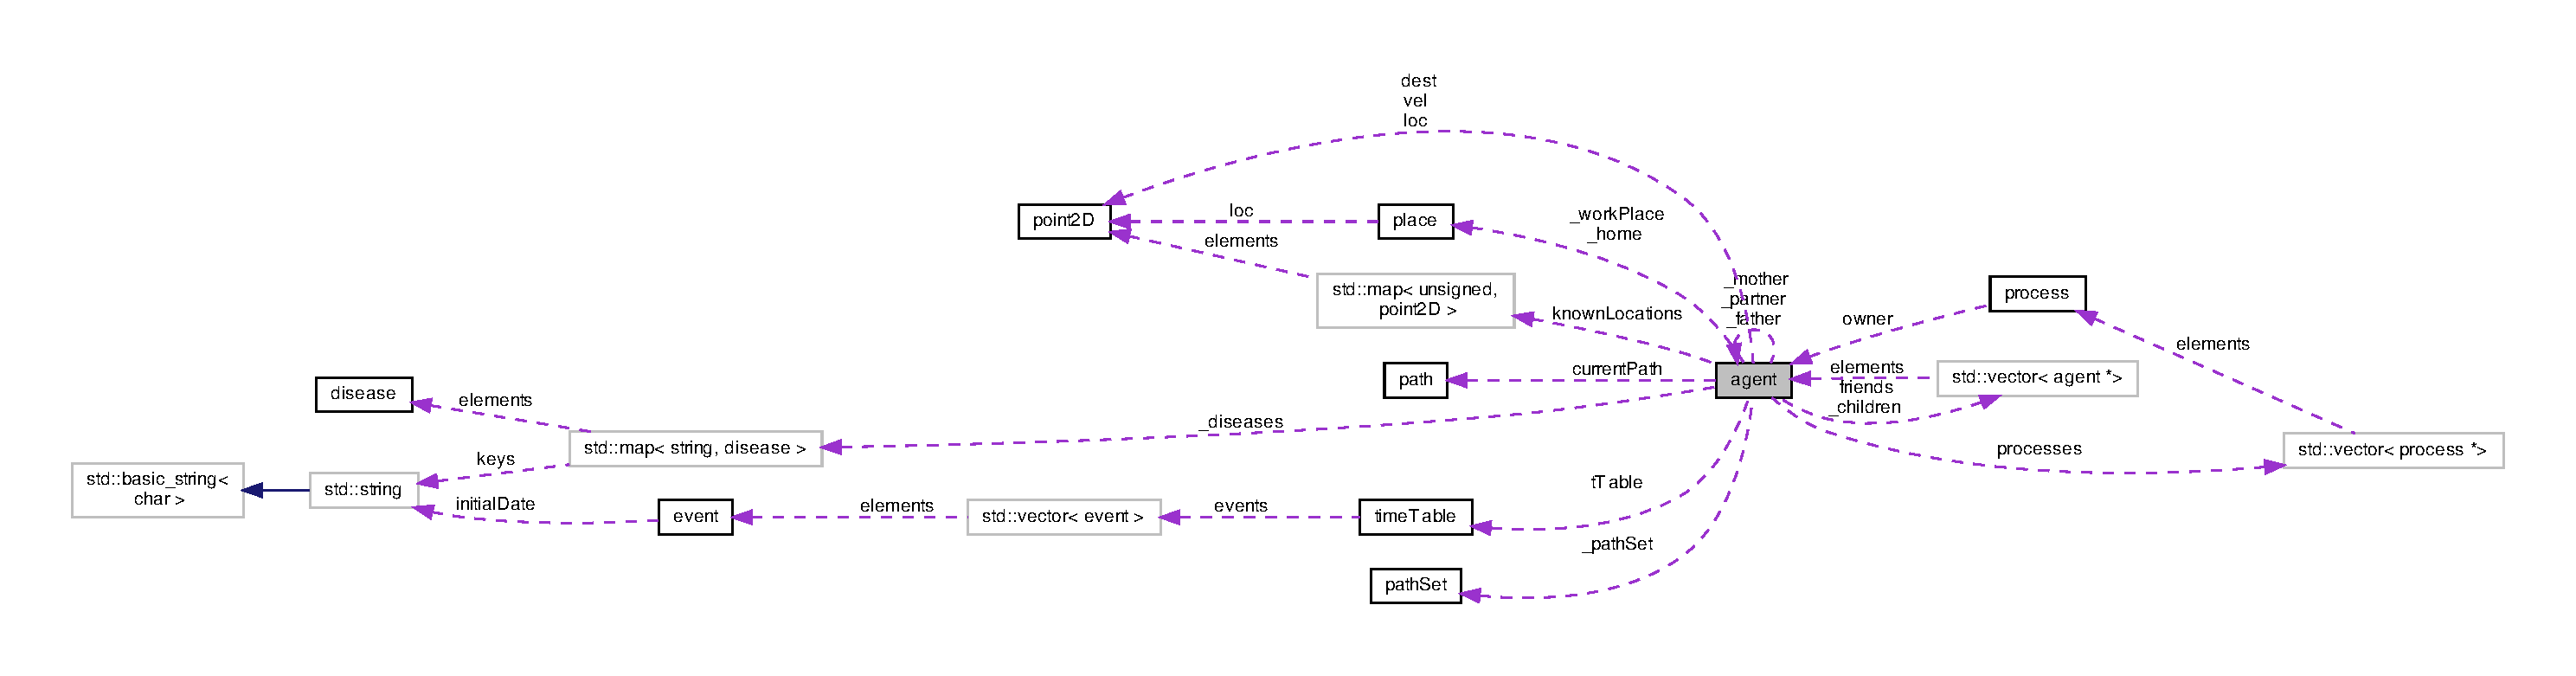
\includegraphics[width=350pt]{classagent__coll__graph}
\end{center}
\end{figure}
\subsection*{Public Member Functions}
\begin{DoxyCompactItemize}
\item 
\mbox{\Hypertarget{classagent_a3d63607b5117bb51096388abb3b56c2d}\label{classagent_a3d63607b5117bb51096388abb3b56c2d}} 
void {\bfseries make\+Partner} (\mbox{\hyperlink{classagent}{agent}} $\ast$)
\item 
\mbox{\Hypertarget{classagent_a7185d1236cdaf47e178a73c19a4c5fdd}\label{classagent_a7185d1236cdaf47e178a73c19a4c5fdd}} 
void {\bfseries make\+Parents} (\mbox{\hyperlink{classagent}{agent}} $\ast$)
\item 
\mbox{\Hypertarget{classagent_a2457ce46575ff9c204ee3e5cae5e5363}\label{classagent_a2457ce46575ff9c204ee3e5cae5e5363}} 
void {\bfseries add\+Child} (\mbox{\hyperlink{classagent}{agent}} $\ast$)
\item 
\mbox{\Hypertarget{classagent_a7fef7c5b65fb384d74d7606168058212}\label{classagent_a7fef7c5b65fb384d74d7606168058212}} 
void {\bfseries update\+Infections} ()
\item 
bool \mbox{\hyperlink{classagent_aab67fe9df4777af3690138fa97d0a3a1}{has\+Disease}} (std\+::string)
\begin{DoxyCompactList}\small\item\em Check to see whether the agent has ever carried a disease with the given name. \end{DoxyCompactList}\item 
bool \mbox{\hyperlink{classagent_a0eee49d52e6c47d7b425bc72cf5caf67}{recovered\+From}} (std\+::string)
\begin{DoxyCompactList}\small\item\em Check to see whether the agent has recovered from a named disease. \end{DoxyCompactList}\item 
void \mbox{\hyperlink{classagent_ac55fabf889e49a48c055c9c495062d5e}{infect\+With}} (std\+::string)
\begin{DoxyCompactList}\small\item\em Infect this agent with a disease with a given name. \end{DoxyCompactList}\item 
bool \mbox{\hyperlink{classagent_ae186a297218e835ac064bf7a329d5b42}{infectious}} ()
\begin{DoxyCompactList}\small\item\em True if the agent can infect other agents. \end{DoxyCompactList}\item 
\mbox{\Hypertarget{classagent_a2a92e38a01bd4c7e03747a3a35d741a0}\label{classagent_a2a92e38a01bd4c7e03747a3a35d741a0}} 
bool {\bfseries exposed} ()
\item 
\mbox{\Hypertarget{classagent_a3c31fe2f6f752a35261041b5bef3c532}\label{classagent_a3c31fe2f6f752a35261041b5bef3c532}} 
void {\bfseries die} ()
\item 
\mbox{\Hypertarget{classagent_a9b9b71b861f9074017a73128c098ef7d}\label{classagent_a9b9b71b861f9074017a73128c098ef7d}} 
bool {\bfseries dead} ()
\item 
\mbox{\Hypertarget{classagent_ac10f380bcc7416f6b2dacaab82d6c7ed}\label{classagent_ac10f380bcc7416f6b2dacaab82d6c7ed}} 
bool {\bfseries in\+Hospital} ()
\item 
\mbox{\Hypertarget{classagent_a8da7d990a32c8b88ce57288b4ddb9dac}\label{classagent_a8da7d990a32c8b88ce57288b4ddb9dac}} 
bool {\bfseries critical} ()
\item 
\mbox{\Hypertarget{classagent_a9b33e19cdc7822f578dd3ea84ae4247b}\label{classagent_a9b33e19cdc7822f578dd3ea84ae4247b}} 
void {\bfseries init} ()
\item 
\mbox{\Hypertarget{classagent_a62677fb1d4e4cb968f297654a34bb2e9}\label{classagent_a62677fb1d4e4cb968f297654a34bb2e9}} 
void {\bfseries pre\+Update} ()
\item 
\mbox{\Hypertarget{classagent_ae20b0b8a169fb7a459c7b195bb970d80}\label{classagent_ae20b0b8a169fb7a459c7b195bb970d80}} 
void {\bfseries update} ()
\item 
\mbox{\Hypertarget{classagent_a30fdee285896c4918428d8713eb9f8b7}\label{classagent_a30fdee285896c4918428d8713eb9f8b7}} 
void {\bfseries apply\+Update} ()
\item 
\mbox{\Hypertarget{classagent_a4474a96ab84b2f4285d672142ac255d8}\label{classagent_a4474a96ab84b2f4285d672142ac255d8}} 
void {\bfseries set\+Dest} (unsigned)
\item 
\mbox{\Hypertarget{classagent_ab29f844fd10dbcd22271dc49da13970c}\label{classagent_ab29f844fd10dbcd22271dc49da13970c}} 
void {\bfseries add\+Process} (\mbox{\hyperlink{classprocess}{process}} $\ast$p)
\item 
\mbox{\Hypertarget{classagent_a89e017002b8df70ed9ccac07f7335f1a}\label{classagent_a89e017002b8df70ed9ccac07f7335f1a}} 
void {\bfseries set\+Job\+Type} (const unsigned \&)
\item 
\mbox{\Hypertarget{classagent_a580f51ad01e693343049bc65e37eb319}\label{classagent_a580f51ad01e693343049bc65e37eb319}} 
void {\bfseries set\+Work\+Place} (\mbox{\hyperlink{classplace}{place}} $\ast$)
\item 
\mbox{\Hypertarget{classagent_a66caa39215e0fba347152cbf7190c85e}\label{classagent_a66caa39215e0fba347152cbf7190c85e}} 
void {\bfseries set\+Work\+Status} (const std\+::string \&)
\item 
\mbox{\Hypertarget{classagent_afbfba46faf7104f44f19dfef8dd72585}\label{classagent_afbfba46faf7104f44f19dfef8dd72585}} 
void {\bfseries set\+Education\+Status} (const std\+::string \&)
\item 
void \mbox{\hyperlink{classagent_ad5a0596438a813a44840ad542416dc50}{set\+Age}} (double)
\begin{DoxyCompactList}\small\item\em Set the age of the agent in years. \end{DoxyCompactList}\item 
void \mbox{\hyperlink{classagent_aaeb64899916c47b42bfdfbc43427d9a8}{set\+Sex}} (const char \&)
\begin{DoxyCompactList}\small\item\em Set the sex of the agent. \end{DoxyCompactList}\item 
char \mbox{\hyperlink{classagent_a0c0cbe17943c2fc044905fe877b14ade}{sex}} ()
\begin{DoxyCompactList}\small\item\em Return the character representing the sex of the agent. \end{DoxyCompactList}\item 
double \mbox{\hyperlink{classagent_a1f8475f933cfae0199d73c108faff1ad}{age}} ()
\begin{DoxyCompactList}\small\item\em Return the age of the agent in years. \end{DoxyCompactList}\item 
\mbox{\hyperlink{classagent}{agent}} $\ast$ \mbox{\hyperlink{classagent_a1e9532f2be4b2b08ee7cdd2a7761237b}{partner}} ()
\begin{DoxyCompactList}\small\item\em Return a pointer to the agent\textquotesingle{}s current partner. \end{DoxyCompactList}\item 
\mbox{\hyperlink{classagent}{agent}} $\ast$ \mbox{\hyperlink{classagent_a6853ae2b9f4b349bd748105699dd43e4}{mother}} ()
\begin{DoxyCompactList}\small\item\em Return a pointer to the agent\textquotesingle{}s mother. \end{DoxyCompactList}\item 
\mbox{\hyperlink{classagent}{agent}} $\ast$ \mbox{\hyperlink{classagent_a1c29803a7627d786ff50d6f39b81a285}{father}} ()
\begin{DoxyCompactList}\small\item\em Return a pointer to the agent\textquotesingle{}s father. \end{DoxyCompactList}\item 
double \mbox{\hyperlink{classagent_a312bd1aeb3c660f43bb3bf5a8f0764e7}{X}} ()
\begin{DoxyCompactList}\small\item\em Return the current X location of the agent. \end{DoxyCompactList}\item 
double \mbox{\hyperlink{classagent_a56b8ea7b9138c5e4b92530d454e247ad}{Y}} ()
\begin{DoxyCompactList}\small\item\em Return the current Y location of the agent. \end{DoxyCompactList}\item 
\mbox{\Hypertarget{classagent_a18cda6439bc5dcf4d444387b380e946f}\label{classagent_a18cda6439bc5dcf4d444387b380e946f}} 
void {\bfseries setX} (double x)
\item 
\mbox{\Hypertarget{classagent_acc06852d54c713a1d8600a1c90b6fcc7}\label{classagent_acc06852d54c713a1d8600a1c90b6fcc7}} 
void {\bfseries setY} (double y)
\item 
\mbox{\Hypertarget{classagent_a5d5e7089351107f21f00c73e342feb59}\label{classagent_a5d5e7089351107f21f00c73e342feb59}} 
bool {\bfseries has\+Work} ()
\item 
\mbox{\Hypertarget{classagent_abcfbb2865a7cb599df7a6c5cbff2ce05}\label{classagent_abcfbb2865a7cb599df7a6c5cbff2ce05}} 
bool {\bfseries worker} ()
\item 
\mbox{\Hypertarget{classagent_a310065019aaf11c07c094c9cc5660471}\label{classagent_a310065019aaf11c07c094c9cc5660471}} 
bool {\bfseries in\+Education} ()
\item 
\mbox{\Hypertarget{classagent_a77eba7e6139ff396a166deee1f508f61}\label{classagent_a77eba7e6139ff396a166deee1f508f61}} 
bool {\bfseries retired} ()
\end{DoxyCompactItemize}
\subsection*{Public Attributes}
\begin{DoxyCompactItemize}
\item 
\mbox{\Hypertarget{classagent_a3b5f19fe489aeaa4a44365b80a20de50}\label{classagent_a3b5f19fe489aeaa4a44365b80a20de50}} 
map$<$ unsigned, \mbox{\hyperlink{classpoint2D}{point2D}} $>$ {\bfseries known\+Locations}
\item 
\mbox{\Hypertarget{classagent_adb1d1bc0cee97d9c4d3c68536e84f3f6}\label{classagent_adb1d1bc0cee97d9c4d3c68536e84f3f6}} 
unsigned {\bfseries old\+Place}
\item 
\mbox{\Hypertarget{classagent_a14bacf305626b17d29eef5681f284f7a}\label{classagent_a14bacf305626b17d29eef5681f284f7a}} 
unsigned {\bfseries new\+Place}
\item 
\mbox{\Hypertarget{classagent_ad7fc52cb970a53fb03f3a08f6e00c4de}\label{classagent_ad7fc52cb970a53fb03f3a08f6e00c4de}} 
\mbox{\hyperlink{structpath}{path}} {\bfseries current\+Path}
\item 
\mbox{\Hypertarget{classagent_ac297c591823cd9c23c8cdbcaea964344}\label{classagent_ac297c591823cd9c23c8cdbcaea964344}} 
unsigned {\bfseries path\+State}
\item 
\mbox{\Hypertarget{classagent_a51641f914b14e5c5be4fd6ea7a6f50f3}\label{classagent_a51641f914b14e5c5be4fd6ea7a6f50f3}} 
\mbox{\hyperlink{structpathSet}{path\+Set}} {\bfseries \+\_\+path\+Set}
\item 
\mbox{\Hypertarget{classagent_a625057d4c53fe2581f1c963d4da601ba}\label{classagent_a625057d4c53fe2581f1c963d4da601ba}} 
\mbox{\hyperlink{classpoint2D}{point2D}} {\bfseries loc}
\item 
\mbox{\Hypertarget{classagent_a1cf261bbb26132bbc68c0a7d920437f4}\label{classagent_a1cf261bbb26132bbc68c0a7d920437f4}} 
\mbox{\hyperlink{classpoint2D}{point2D}} {\bfseries dest}
\item 
\mbox{\Hypertarget{classagent_a5ff902fc713259415266ca26f2bb8ecb}\label{classagent_a5ff902fc713259415266ca26f2bb8ecb}} 
\mbox{\hyperlink{classpoint2D}{point2D}} {\bfseries vel}
\item 
\mbox{\Hypertarget{classagent_aa029a96be166646fb046873a73d3fbdd}\label{classagent_aa029a96be166646fb046873a73d3fbdd}} 
float {\bfseries \+\_\+size}
\item 
double \mbox{\hyperlink{classagent_a9c76eb9369864fb60a2d5a4f44c56843}{\+\_\+age}}
\begin{DoxyCompactList}\small\item\em The age of the agent in years. \end{DoxyCompactList}\item 
\mbox{\Hypertarget{classagent_a6235c5897c39008af08d75fa7dca13b2}\label{classagent_a6235c5897c39008af08d75fa7dca13b2}} 
vector$<$ \mbox{\hyperlink{classagent}{agent}} $\ast$ $>$ {\bfseries friends}
\item 
\mbox{\Hypertarget{classagent_a0a669d47bb2f6781ea5ec1f2cdfdd4e2}\label{classagent_a0a669d47bb2f6781ea5ec1f2cdfdd4e2}} 
\mbox{\hyperlink{structtimeTable}{time\+Table}} {\bfseries t\+Table}
\item 
\mbox{\Hypertarget{classagent_a4a2f231b103bbe13452570921e296ea1}\label{classagent_a4a2f231b103bbe13452570921e296ea1}} 
bool \mbox{\hyperlink{classagent_a4a2f231b103bbe13452570921e296ea1}{\+\_\+in\+Hospital}}
\begin{DoxyCompactList}\small\item\em Set to true if the agent is currently in hospital. \end{DoxyCompactList}\item 
\mbox{\Hypertarget{classagent_a9803ed96415b37e5ad091848a53e1944}\label{classagent_a9803ed96415b37e5ad091848a53e1944}} 
bool \mbox{\hyperlink{classagent_a9803ed96415b37e5ad091848a53e1944}{\+\_\+critical}}
\begin{DoxyCompactList}\small\item\em Set to true if the agent is in hospital and in critical care. \end{DoxyCompactList}\item 
\mbox{\Hypertarget{classagent_a0d09f2c676410b866a348291900ee520}\label{classagent_a0d09f2c676410b866a348291900ee520}} 
bool \mbox{\hyperlink{classagent_a0d09f2c676410b866a348291900ee520}{\+\_\+died}}
\begin{DoxyCompactList}\small\item\em Set to true if the agent has died (for any reason...) \end{DoxyCompactList}\item 
unsigned \mbox{\hyperlink{classagent_a4145c90d534f84deb22a93560809134c}{number\+Infected}}
\begin{DoxyCompactList}\small\item\em Accumulates the number of other agents infected by this agent. \end{DoxyCompactList}\item 
map$<$ string, \mbox{\hyperlink{classdisease}{disease}} $>$ \mbox{\hyperlink{classagent_a2352342e95bc77041c07c0dafdfb7cd2}{\+\_\+diseases}}
\begin{DoxyCompactList}\small\item\em A dictionary of named diseases currently carried by this agent. \end{DoxyCompactList}\item 
\mbox{\Hypertarget{classagent_a7f99e11ffb5c042be84e2917cba7af3a}\label{classagent_a7f99e11ffb5c042be84e2917cba7af3a}} 
unsigned {\bfseries ID}
\item 
\mbox{\Hypertarget{classagent_a3db995cae037474ae4bf7adcb7cd44cc}\label{classagent_a3db995cae037474ae4bf7adcb7cd44cc}} 
int {\bfseries cell\+Index}
\item 
\mbox{\Hypertarget{classagent_a13305f6e66e992cf1c6ffa7b027c4201}\label{classagent_a13305f6e66e992cf1c6ffa7b027c4201}} 
vector$<$ \mbox{\hyperlink{classprocess}{process}} $\ast$ $>$ {\bfseries processes}
\end{DoxyCompactItemize}
\subsection*{Static Public Attributes}
\begin{DoxyCompactItemize}
\item 
\mbox{\Hypertarget{classagent_a4fd7d01331ffd547ae9fc8eb9b05516d}\label{classagent_a4fd7d01331ffd547ae9fc8eb9b05516d}} 
static unsigned {\bfseries idnum} =0
\end{DoxyCompactItemize}
\subsection*{Private Types}
\begin{DoxyCompactItemize}
\item 
\mbox{\Hypertarget{classagent_a56ecbbe6f1ec07d60ed3c30988810e22}\label{classagent_a56ecbbe6f1ec07d60ed3c30988810e22}} 
enum {\bfseries work\+Types} \{ {\bfseries ineducation}, 
{\bfseries unemployed}, 
{\bfseries working}, 
{\bfseries retiree}
 \}
\item 
\mbox{\Hypertarget{classagent_a499a1e074636f81ed46fe569107e6cde}\label{classagent_a499a1e074636f81ed46fe569107e6cde}} 
enum {\bfseries education\+Types} \{ \newline
{\bfseries preschool}, 
{\bfseries primary}, 
{\bfseries secondary}, 
{\bfseries uppersecondary}, 
\newline
{\bfseries higher}, 
{\bfseries postgrad}
 \}
\end{DoxyCompactItemize}
\subsection*{Private Attributes}
\begin{DoxyCompactItemize}
\item 
\mbox{\Hypertarget{classagent_a232bde3d6f75bac6c1fba313b7124b13}\label{classagent_a232bde3d6f75bac6c1fba313b7124b13}} 
\mbox{\hyperlink{classplace}{place}} $\ast$ {\bfseries \+\_\+work\+Place}
\item 
\mbox{\Hypertarget{classagent_a6db9c370528e73527b4d7a8b00ffab23}\label{classagent_a6db9c370528e73527b4d7a8b00ffab23}} 
\mbox{\hyperlink{classplace}{place}} $\ast$ {\bfseries \+\_\+home}
\item 
\mbox{\Hypertarget{classagent_a4155df9fba51d2a5387b266e74f0703e}\label{classagent_a4155df9fba51d2a5387b266e74f0703e}} 
unsigned {\bfseries \+\_\+job\+Type}
\item 
\mbox{\Hypertarget{classagent_a79ee05496cc1bc2d806fbb70a45d9f99}\label{classagent_a79ee05496cc1bc2d806fbb70a45d9f99}} 
work\+Types {\bfseries \+\_\+work\+Status}
\item 
\mbox{\Hypertarget{classagent_abbfd4798d2b47e4b418a9aefa75fd75b}\label{classagent_abbfd4798d2b47e4b418a9aefa75fd75b}} 
education\+Types {\bfseries \+\_\+education\+Status}
\item 
\mbox{\Hypertarget{classagent_ad2e0f7c2a20dcfa12f07a07520ee7e4a}\label{classagent_ad2e0f7c2a20dcfa12f07a07520ee7e4a}} 
char \mbox{\hyperlink{classagent_ad2e0f7c2a20dcfa12f07a07520ee7e4a}{\+\_\+sex}}
\begin{DoxyCompactList}\small\item\em A character representing the agent\textquotesingle{}s sex -\/ withe \textquotesingle{}m\textquotesingle{} or \textquotesingle{}f\textquotesingle{}. \end{DoxyCompactList}\item 
\mbox{\Hypertarget{classagent_a54b776c2ea81520b05c683632bed82fd}\label{classagent_a54b776c2ea81520b05c683632bed82fd}} 
\mbox{\hyperlink{classagent}{agent}} $\ast$ {\bfseries \+\_\+partner}
\item 
\mbox{\Hypertarget{classagent_abff69cc5e2c8b7dcbd4c6eeeb9323a08}\label{classagent_abff69cc5e2c8b7dcbd4c6eeeb9323a08}} 
\mbox{\hyperlink{classagent}{agent}} $\ast$ {\bfseries \+\_\+mother}
\item 
\mbox{\Hypertarget{classagent_ae55ddedf072040f0cb8930217660e697}\label{classagent_ae55ddedf072040f0cb8930217660e697}} 
\mbox{\hyperlink{classagent}{agent}} $\ast$ {\bfseries \+\_\+father}
\item 
\mbox{\Hypertarget{classagent_af42fc69cd57f652287501750499c6024}\label{classagent_af42fc69cd57f652287501750499c6024}} 
vector$<$ \mbox{\hyperlink{classagent}{agent}} $\ast$ $>$ {\bfseries \+\_\+children}
\end{DoxyCompactItemize}


\subsection{Detailed Description}
Agents represent individual people. 

Definition at line 22 of file agent.\+h.



\subsection{Member Function Documentation}
\mbox{\Hypertarget{classagent_a1f8475f933cfae0199d73c108faff1ad}\label{classagent_a1f8475f933cfae0199d73c108faff1ad}} 
\index{agent@{agent}!age@{age}}
\index{age@{age}!agent@{agent}}
\subsubsection{\texorpdfstring{age()}{age()}}
{\footnotesize\ttfamily double agent\+::age (\begin{DoxyParamCaption}{ }\end{DoxyParamCaption})}



Return the age of the agent in years. 

\begin{DoxyReturn}{Returns}
double 
\end{DoxyReturn}


Definition at line 225 of file agent.\+cpp.

\mbox{\Hypertarget{classagent_a1c29803a7627d786ff50d6f39b81a285}\label{classagent_a1c29803a7627d786ff50d6f39b81a285}} 
\index{agent@{agent}!father@{father}}
\index{father@{father}!agent@{agent}}
\subsubsection{\texorpdfstring{father()}{father()}}
{\footnotesize\ttfamily \mbox{\hyperlink{classagent}{agent}} $\ast$ agent\+::father (\begin{DoxyParamCaption}{ }\end{DoxyParamCaption})}



Return a pointer to the agent\textquotesingle{}s father. 

Returns nullptr is partner does not exist (set in constructor)

\begin{DoxyReturn}{Returns}
agent$\ast$ 
\end{DoxyReturn}


Definition at line 237 of file agent.\+cpp.

\mbox{\Hypertarget{classagent_aab67fe9df4777af3690138fa97d0a3a1}\label{classagent_aab67fe9df4777af3690138fa97d0a3a1}} 
\index{agent@{agent}!has\+Disease@{has\+Disease}}
\index{has\+Disease@{has\+Disease}!agent@{agent}}
\subsubsection{\texorpdfstring{has\+Disease()}{hasDisease()}}
{\footnotesize\ttfamily bool agent\+::has\+Disease (\begin{DoxyParamCaption}\item[{std\+::string}]{name }\end{DoxyParamCaption})}



Check to see whether the agent has ever carried a disease with the given name. 

Returns false if there is no entry in the dictionary of diseases, true if it is present, even if the agent has recovered or died This allows for testing recovered agents (or for them to have limited time immunity), or for dead agents still to be infectious


\begin{DoxyParams}{Parameters}
{\em name} & \+:A string specifying the name of the disease to test for \\
\hline
\end{DoxyParams}
\begin{DoxyReturn}{Returns}
bool 
\end{DoxyReturn}


Definition at line 167 of file agent.\+cpp.

\mbox{\Hypertarget{classagent_ae186a297218e835ac064bf7a329d5b42}\label{classagent_ae186a297218e835ac064bf7a329d5b42}} 
\index{agent@{agent}!infectious@{infectious}}
\index{infectious@{infectious}!agent@{agent}}
\subsubsection{\texorpdfstring{infectious()}{infectious()}}
{\footnotesize\ttfamily bool agent\+::infectious (\begin{DoxyParamCaption}{ }\end{DoxyParamCaption})}



True if the agent can infect other agents. 

Currently only applies for Covid19! This function is used in creating maps in output.\+cpp via the \mbox{\hyperlink{classsearchGrid}{search\+Grid}}, so be careful about modifying \begin{DoxyRefDesc}{Todo}
\item[\mbox{\hyperlink{todo__todo000002}{Todo}}]Should take a disease name as the argument\end{DoxyRefDesc}


\begin{DoxyReturn}{Returns}
bool 
\end{DoxyReturn}


Definition at line 80 of file agent.\+cpp.

\mbox{\Hypertarget{classagent_ac55fabf889e49a48c055c9c495062d5e}\label{classagent_ac55fabf889e49a48c055c9c495062d5e}} 
\index{agent@{agent}!infect\+With@{infect\+With}}
\index{infect\+With@{infect\+With}!agent@{agent}}
\subsubsection{\texorpdfstring{infect\+With()}{infectWith()}}
{\footnotesize\ttfamily void agent\+::infect\+With (\begin{DoxyParamCaption}\item[{std\+::string}]{name }\end{DoxyParamCaption})}



Infect this agent with a disease with a given name. 

This both adds the disease name to the dictionary and creates a new disease object with the name of the disease The disease object is then updated to the \char`\"{}infected\char`\"{} state, which indicates that this is a newly acquired disease.


\begin{DoxyParams}{Parameters}
{\em name} & \+:A string specifying the name of the disease \\
\hline
\end{DoxyParams}


Definition at line 177 of file agent.\+cpp.

\mbox{\Hypertarget{classagent_a6853ae2b9f4b349bd748105699dd43e4}\label{classagent_a6853ae2b9f4b349bd748105699dd43e4}} 
\index{agent@{agent}!mother@{mother}}
\index{mother@{mother}!agent@{agent}}
\subsubsection{\texorpdfstring{mother()}{mother()}}
{\footnotesize\ttfamily \mbox{\hyperlink{classagent}{agent}} $\ast$ agent\+::mother (\begin{DoxyParamCaption}{ }\end{DoxyParamCaption})}



Return a pointer to the agent\textquotesingle{}s mother. 

Returns nullptr is partner does not exist (set in constructor)

\begin{DoxyReturn}{Returns}
agent$\ast$ 
\end{DoxyReturn}


Definition at line 233 of file agent.\+cpp.

\mbox{\Hypertarget{classagent_a1e9532f2be4b2b08ee7cdd2a7761237b}\label{classagent_a1e9532f2be4b2b08ee7cdd2a7761237b}} 
\index{agent@{agent}!partner@{partner}}
\index{partner@{partner}!agent@{agent}}
\subsubsection{\texorpdfstring{partner()}{partner()}}
{\footnotesize\ttfamily \mbox{\hyperlink{classagent}{agent}} $\ast$ agent\+::partner (\begin{DoxyParamCaption}{ }\end{DoxyParamCaption})}



Return a pointer to the agent\textquotesingle{}s current partner. 

Returns nullptr is partner does not exist (set in constructor)

\begin{DoxyReturn}{Returns}
agent$\ast$ 
\end{DoxyReturn}


Definition at line 229 of file agent.\+cpp.

\mbox{\Hypertarget{classagent_a0eee49d52e6c47d7b425bc72cf5caf67}\label{classagent_a0eee49d52e6c47d7b425bc72cf5caf67}} 
\index{agent@{agent}!recovered\+From@{recovered\+From}}
\index{recovered\+From@{recovered\+From}!agent@{agent}}
\subsubsection{\texorpdfstring{recovered\+From()}{recoveredFrom()}}
{\footnotesize\ttfamily bool agent\+::recovered\+From (\begin{DoxyParamCaption}\item[{std\+::string}]{name }\end{DoxyParamCaption})}



Check to see whether the agent has recovered from a named disease. 


\begin{DoxyParams}{Parameters}
{\em name} & \+:A string specifying the name of the disease to test for\\
\hline
\end{DoxyParams}
\begin{DoxyReturn}{Returns}
bool 
\end{DoxyReturn}


Definition at line 171 of file agent.\+cpp.

\mbox{\Hypertarget{classagent_ad5a0596438a813a44840ad542416dc50}\label{classagent_ad5a0596438a813a44840ad542416dc50}} 
\index{agent@{agent}!set\+Age@{set\+Age}}
\index{set\+Age@{set\+Age}!agent@{agent}}
\subsubsection{\texorpdfstring{set\+Age()}{setAge()}}
{\footnotesize\ttfamily void agent\+::set\+Age (\begin{DoxyParamCaption}\item[{double}]{a }\end{DoxyParamCaption})}



Set the age of the agent in years. 


\begin{DoxyParams}{Parameters}
{\em a} & a double representing the age in years \\
\hline
\end{DoxyParams}


Definition at line 28 of file agent.\+cpp.

\mbox{\Hypertarget{classagent_aaeb64899916c47b42bfdfbc43427d9a8}\label{classagent_aaeb64899916c47b42bfdfbc43427d9a8}} 
\index{agent@{agent}!set\+Sex@{set\+Sex}}
\index{set\+Sex@{set\+Sex}!agent@{agent}}
\subsubsection{\texorpdfstring{set\+Sex()}{setSex()}}
{\footnotesize\ttfamily void agent\+::set\+Sex (\begin{DoxyParamCaption}\item[{const char \&}]{s }\end{DoxyParamCaption})}



Set the sex of the agent. 

By default the constructor sets this value to \textquotesingle{}f\textquotesingle{}. The code will abort if input is anything other than \textquotesingle{}m\textquotesingle{} or \textquotesingle{}f\textquotesingle{}


\begin{DoxyParams}{Parameters}
{\em s} & A character, either \textquotesingle{}m\textquotesingle{} or \textquotesingle{}f\textquotesingle{} \\
\hline
\end{DoxyParams}


Definition at line 32 of file agent.\+cpp.

\mbox{\Hypertarget{classagent_a0c0cbe17943c2fc044905fe877b14ade}\label{classagent_a0c0cbe17943c2fc044905fe877b14ade}} 
\index{agent@{agent}!sex@{sex}}
\index{sex@{sex}!agent@{agent}}
\subsubsection{\texorpdfstring{sex()}{sex()}}
{\footnotesize\ttfamily char agent\+::sex (\begin{DoxyParamCaption}{ }\end{DoxyParamCaption})}



Return the character representing the sex of the agent. 

Returned value should be either \textquotesingle{}m\textquotesingle{} or \textquotesingle{}f\textquotesingle{}

\begin{DoxyReturn}{Returns}
char 
\end{DoxyReturn}


Definition at line 220 of file agent.\+cpp.

\mbox{\Hypertarget{classagent_a312bd1aeb3c660f43bb3bf5a8f0764e7}\label{classagent_a312bd1aeb3c660f43bb3bf5a8f0764e7}} 
\index{agent@{agent}!X@{X}}
\index{X@{X}!agent@{agent}}
\subsubsection{\texorpdfstring{X()}{X()}}
{\footnotesize\ttfamily double agent\+::X (\begin{DoxyParamCaption}{ }\end{DoxyParamCaption})}



Return the current X location of the agent. 

\begin{DoxyReturn}{Returns}
double 
\end{DoxyReturn}


Definition at line 197 of file agent.\+cpp.

\mbox{\Hypertarget{classagent_a56b8ea7b9138c5e4b92530d454e247ad}\label{classagent_a56b8ea7b9138c5e4b92530d454e247ad}} 
\index{agent@{agent}!Y@{Y}}
\index{Y@{Y}!agent@{agent}}
\subsubsection{\texorpdfstring{Y()}{Y()}}
{\footnotesize\ttfamily double agent\+::Y (\begin{DoxyParamCaption}{ }\end{DoxyParamCaption})}



Return the current Y location of the agent. 

\begin{DoxyReturn}{Returns}
double 
\end{DoxyReturn}


Definition at line 201 of file agent.\+cpp.



\subsection{Member Data Documentation}
\mbox{\Hypertarget{classagent_a9c76eb9369864fb60a2d5a4f44c56843}\label{classagent_a9c76eb9369864fb60a2d5a4f44c56843}} 
\index{agent@{agent}!\+\_\+age@{\+\_\+age}}
\index{\+\_\+age@{\+\_\+age}!agent@{agent}}
\subsubsection{\texorpdfstring{\+\_\+age}{\_age}}
{\footnotesize\ttfamily double agent\+::\+\_\+age}



The age of the agent in years. 

The age is a double\+: sub-\/units of a year are thus decimal fractions. Updating the age thus depends on being sure the timestep is in seconds At present no allowance is made for dates (this no leap years etc.) -\/ age is just updated using elapsed seconds in a timestep divided by seconds in 365 days. Defaults to zero in the constructor. Updated in agent\+::pre\+Update 

Definition at line 57 of file agent.\+h.

\mbox{\Hypertarget{classagent_a2352342e95bc77041c07c0dafdfb7cd2}\label{classagent_a2352342e95bc77041c07c0dafdfb7cd2}} 
\index{agent@{agent}!\+\_\+diseases@{\+\_\+diseases}}
\index{\+\_\+diseases@{\+\_\+diseases}!agent@{agent}}
\subsubsection{\texorpdfstring{\+\_\+diseases}{\_diseases}}
{\footnotesize\ttfamily map$<$string,\mbox{\hyperlink{classdisease}{disease}}$>$ agent\+::\+\_\+diseases}



A dictionary of named diseases currently carried by this agent. 

If the agent has never had a given disease, then there will be no entry in the dictionary. Such agents are assumed to be susceptible. 

Definition at line 96 of file agent.\+h.

\mbox{\Hypertarget{classagent_a4145c90d534f84deb22a93560809134c}\label{classagent_a4145c90d534f84deb22a93560809134c}} 
\index{agent@{agent}!number\+Infected@{number\+Infected}}
\index{number\+Infected@{number\+Infected}!agent@{agent}}
\subsubsection{\texorpdfstring{number\+Infected}{numberInfected}}
{\footnotesize\ttfamily unsigned agent\+::number\+Infected}



Accumulates the number of other agents infected by this agent. 

Currently this is not distinguished by disease so really only works if there is just a single disease \begin{DoxyRefDesc}{Todo}
\item[\mbox{\hyperlink{todo__todo000001}{Todo}}]change to a version that can accumlate infections by named disease (NB this value is used in \mbox{\hyperlink{model_8cpp}{model.\+cpp}} to find R0) \end{DoxyRefDesc}


Definition at line 89 of file agent.\+h.



The documentation for this class was generated from the following files\+:\begin{DoxyCompactItemize}
\item 
\mbox{\hyperlink{agent_8h}{agent.\+h}}\item 
agent.\+cpp\item 
agents.\+h\end{DoxyCompactItemize}

\hypertarget{classagentFactory}{}\section{agent\+Factory Class Reference}
\label{classagentFactory}\index{agent\+Factory@{agent\+Factory}}


Inheritance diagram for agent\+Factory\+:
\nopagebreak
\begin{figure}[H]
\begin{center}
\leavevmode
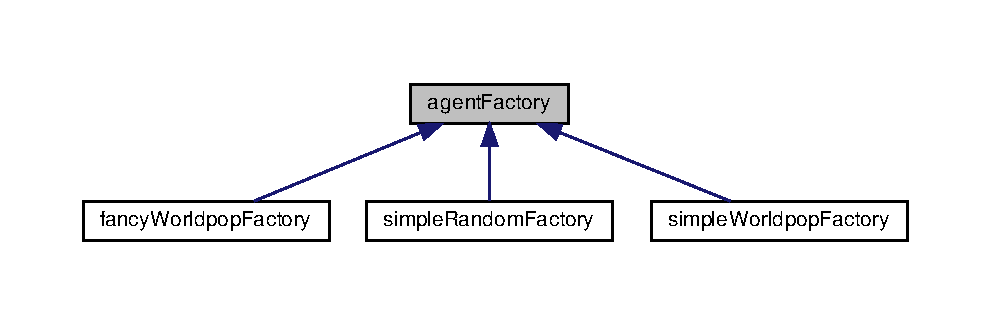
\includegraphics[width=350pt]{classagentFactory__inherit__graph}
\end{center}
\end{figure}
\subsection*{Public Member Functions}
\begin{DoxyCompactItemize}
\item 
\mbox{\Hypertarget{classagentFactory_ab3b48ba713d17c58995adbff5f0dbb9b}\label{classagentFactory_ab3b48ba713d17c58995adbff5f0dbb9b}} 
virtual void {\bfseries create\+Agents} (vector$<$ \mbox{\hyperlink{classagent}{agent}} $\ast$$>$ \&)=0
\end{DoxyCompactItemize}


\subsection{Detailed Description}


Definition at line 9 of file agent\+Factory.\+h.



The documentation for this class was generated from the following file\+:\begin{DoxyCompactItemize}
\item 
agent\+Factory.\+h\end{DoxyCompactItemize}

\hypertarget{classagentFactorySelector}{}\section{agent\+Factory\+Selector Class Reference}
\label{classagentFactorySelector}\index{agent\+Factory\+Selector@{agent\+Factory\+Selector}}
\subsection*{Static Public Member Functions}
\begin{DoxyCompactItemize}
\item 
\mbox{\Hypertarget{classagentFactorySelector_a10639ee22ff121232ffe1bbd73d0f19e}\label{classagentFactorySelector_a10639ee22ff121232ffe1bbd73d0f19e}} 
static \mbox{\hyperlink{classagentFactory}{agent\+Factory}} \& {\bfseries select} (std\+::string name)
\end{DoxyCompactItemize}


\subsection{Detailed Description}


Definition at line 110 of file agent\+Factory.\+h.



The documentation for this class was generated from the following file\+:\begin{DoxyCompactItemize}
\item 
agent\+Factory.\+h\end{DoxyCompactItemize}

\hypertarget{classagents}{}\section{agents Class Reference}
\label{classagents}\index{agents@{agents}}


Inheritance diagram for agents\+:\nopagebreak
\begin{figure}[H]
\begin{center}
\leavevmode
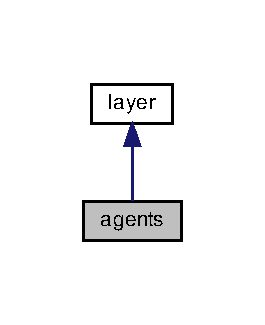
\includegraphics[width=127pt]{classagents__inherit__graph}
\end{center}
\end{figure}


Collaboration diagram for agents\+:\nopagebreak
\begin{figure}[H]
\begin{center}
\leavevmode
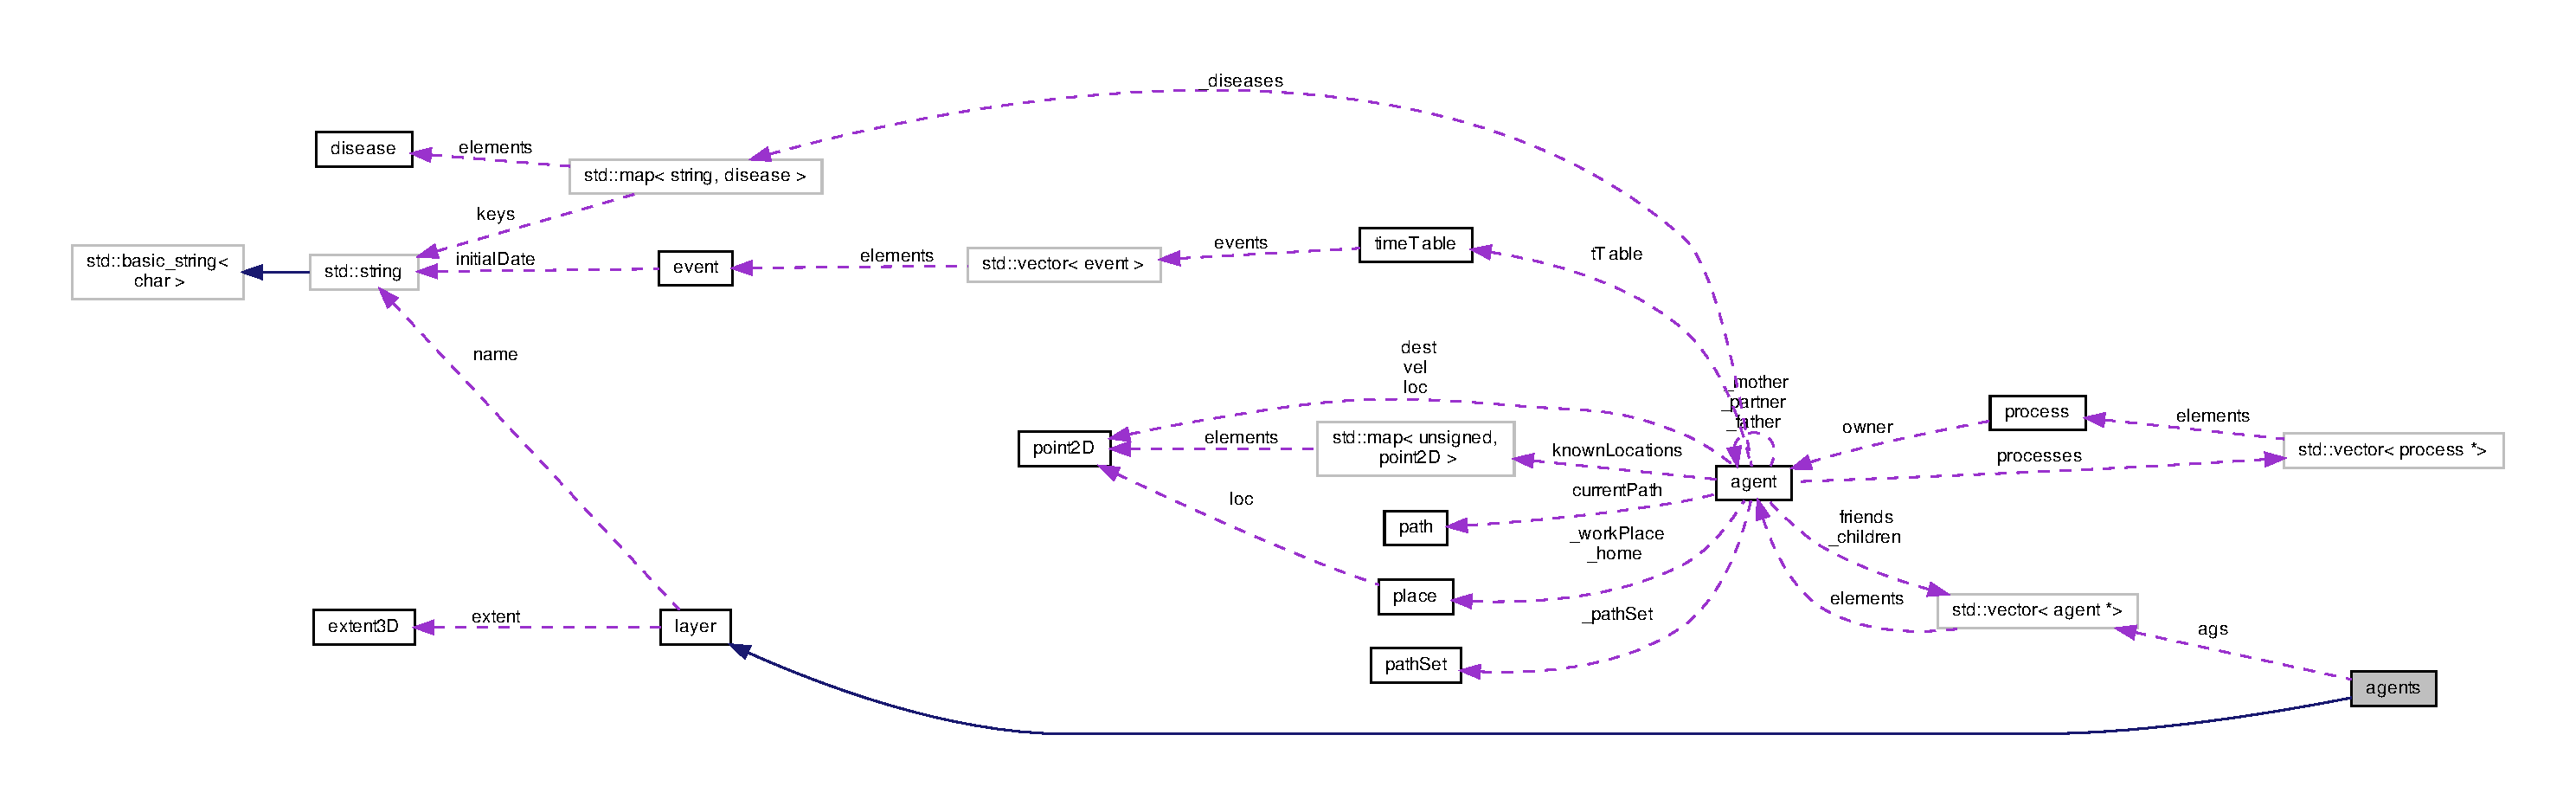
\includegraphics[width=350pt]{classagents__coll__graph}
\end{center}
\end{figure}
\subsection*{Public Member Functions}
\begin{DoxyCompactItemize}
\item 
\mbox{\Hypertarget{classagents_a90630d810c0ced5db4c190ed52720f9d}\label{classagents_a90630d810c0ced5db4c190ed52720f9d}} 
bool {\bfseries update} ()
\end{DoxyCompactItemize}
\subsection*{Public Attributes}
\begin{DoxyCompactItemize}
\item 
\mbox{\Hypertarget{classagents_a550d3cd56fd72b1d1e8a454ef1b718fd}\label{classagents_a550d3cd56fd72b1d1e8a454ef1b718fd}} 
vector$<$ \mbox{\hyperlink{classagent}{agent}} $\ast$ $>$ {\bfseries ags}
\end{DoxyCompactItemize}
\subsection*{Private Attributes}
\begin{DoxyCompactItemize}
\item 
\mbox{\Hypertarget{classagents_abbbc60318d34a17b9efccfe1c98e2a46}\label{classagents_abbbc60318d34a17b9efccfe1c98e2a46}} 
float {\bfseries dt}
\end{DoxyCompactItemize}
\subsection*{Additional Inherited Members}


\subsection{Detailed Description}


Definition at line 18 of file agents.\+h.



The documentation for this class was generated from the following file\+:\begin{DoxyCompactItemize}
\item 
agents.\+h\end{DoxyCompactItemize}

\hypertarget{classasciiGrid}{}\section{ascii\+Grid Class Reference}
\label{classasciiGrid}\index{ascii\+Grid@{ascii\+Grid}}


Collaboration diagram for ascii\+Grid\+:\nopagebreak
\begin{figure}[H]
\begin{center}
\leavevmode
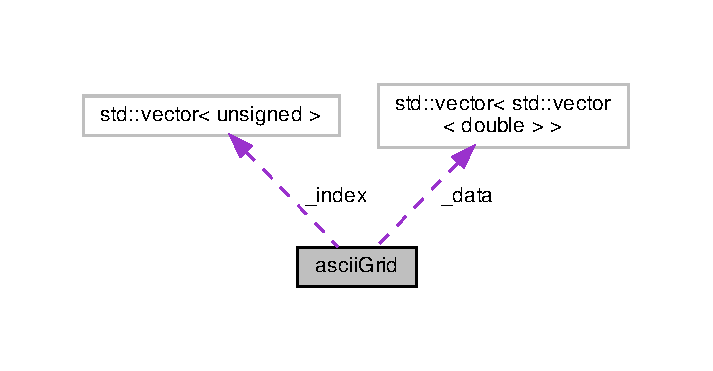
\includegraphics[width=342pt]{classasciiGrid__coll__graph}
\end{center}
\end{figure}
\subsection*{Public Member Functions}
\begin{DoxyCompactItemize}
\item 
\mbox{\Hypertarget{classasciiGrid_af8550fe183b2826823cab513878dcc8d}\label{classasciiGrid_af8550fe183b2826823cab513878dcc8d}} 
{\bfseries ascii\+Grid} (std\+::string)
\item 
\mbox{\Hypertarget{classasciiGrid_af009652a3b09761f42af9b6a9510aca7}\label{classasciiGrid_af009652a3b09761f42af9b6a9510aca7}} 
void {\bfseries read\+File} (const std\+::string \&)
\item 
\mbox{\Hypertarget{classasciiGrid_a3f76f212cbd1eafd58da22623d49f44c}\label{classasciiGrid_a3f76f212cbd1eafd58da22623d49f44c}} 
void {\bfseries read\+Data} (std\+::ifstream \&)
\item 
\mbox{\Hypertarget{classasciiGrid_aa8f140d48bc75fd0cb54c2e092ae81a6}\label{classasciiGrid_aa8f140d48bc75fd0cb54c2e092ae81a6}} 
void {\bfseries read\+Header} (std\+::ifstream \&)
\item 
\mbox{\Hypertarget{classasciiGrid_a9d4130b7ef3a98f9ece49cdf03f63849}\label{classasciiGrid_a9d4130b7ef3a98f9ece49cdf03f63849}} 
const std\+::vector$<$ std\+::string $>$ {\bfseries String\+To\+Words} (const std\+::string \&, const char) const
\item 
\mbox{\Hypertarget{classasciiGrid_ace6a959d265f1f6da26f1aaf5721efe5}\label{classasciiGrid_ace6a959d265f1f6da26f1aaf5721efe5}} 
const std\+::vector$<$ double $>$ {\bfseries Line\+To\+Double} (const std\+::string \&, const char) const
\item 
\mbox{\Hypertarget{classasciiGrid_a0ec01a9678211fe765761a9c144a99f7}\label{classasciiGrid_a0ec01a9678211fe765761a9c144a99f7}} 
double {\bfseries String\+To\+Double} (const std\+::string \&string) const
\item 
\mbox{\Hypertarget{classasciiGrid_aea0714b6499575ddadc02f5ab0a918c5}\label{classasciiGrid_aea0714b6499575ddadc02f5ab0a918c5}} 
int {\bfseries String\+To\+Int} (const std\+::string \&string) const
\item 
\mbox{\Hypertarget{classasciiGrid_ac9d2e6796db7a7e0498965b4052e35db}\label{classasciiGrid_ac9d2e6796db7a7e0498965b4052e35db}} 
\mbox{\hyperlink{classpoint2D}{point2D}} {\bfseries get\+Valid\+Point} (unsigned)
\item 
\mbox{\Hypertarget{classasciiGrid_a340a0d2b319b7d3870d600a11394dfb8}\label{classasciiGrid_a340a0d2b319b7d3870d600a11394dfb8}} 
\mbox{\hyperlink{classpoint2D}{point2D}} {\bfseries get\+Valid\+Randomised\+Point} (unsigned)
\item 
\mbox{\Hypertarget{classasciiGrid_add163ffae683376f280c2213ff934bbb}\label{classasciiGrid_add163ffae683376f280c2213ff934bbb}} 
double {\bfseries get\+Data\+At} (unsigned)
\item 
\mbox{\Hypertarget{classasciiGrid_a105a28e8ffea13d3028056d96fff635f}\label{classasciiGrid_a105a28e8ffea13d3028056d96fff635f}} 
bool {\bfseries is\+Valid} (unsigned)
\item 
\mbox{\Hypertarget{classasciiGrid_ab8ed7fabf5543d2a67a91625d27fc09b}\label{classasciiGrid_ab8ed7fabf5543d2a67a91625d27fc09b}} 
double {\bfseries x\+Origin} ()
\item 
\mbox{\Hypertarget{classasciiGrid_a11da6bbac5ded2d9ada9f135268bc6d2}\label{classasciiGrid_a11da6bbac5ded2d9ada9f135268bc6d2}} 
double {\bfseries y\+Origin} ()
\item 
\mbox{\Hypertarget{classasciiGrid_a50fc35c27a953963fb5ce7e648b2362e}\label{classasciiGrid_a50fc35c27a953963fb5ce7e648b2362e}} 
double {\bfseries x\+Size} ()
\item 
\mbox{\Hypertarget{classasciiGrid_a9959f994fa19b93fc7d2185ea162e979}\label{classasciiGrid_a9959f994fa19b93fc7d2185ea162e979}} 
double {\bfseries y\+Size} ()
\end{DoxyCompactItemize}
\subsection*{Public Attributes}
\begin{DoxyCompactItemize}
\item 
\mbox{\Hypertarget{classasciiGrid_a061a3c19021ec5df0132375100106918}\label{classasciiGrid_a061a3c19021ec5df0132375100106918}} 
std\+::vector$<$ unsigned $>$ {\bfseries \+\_\+index}
\end{DoxyCompactItemize}
\subsection*{Private Attributes}
\begin{DoxyCompactItemize}
\item 
\mbox{\Hypertarget{classasciiGrid_a954aec05c9ed74b69460f98365d71d04}\label{classasciiGrid_a954aec05c9ed74b69460f98365d71d04}} 
int {\bfseries \+\_\+ncols}
\item 
\mbox{\Hypertarget{classasciiGrid_ab97218c7133b2aafb78f87f3daa7b1bb}\label{classasciiGrid_ab97218c7133b2aafb78f87f3daa7b1bb}} 
int {\bfseries \+\_\+nrows}
\item 
\mbox{\Hypertarget{classasciiGrid_a5aba0243eeede7d3f475ca4673a19091}\label{classasciiGrid_a5aba0243eeede7d3f475ca4673a19091}} 
double {\bfseries \+\_\+xllcorner}
\item 
\mbox{\Hypertarget{classasciiGrid_a2915f11c96cd5a1fe8c76db4ffd8248e}\label{classasciiGrid_a2915f11c96cd5a1fe8c76db4ffd8248e}} 
double {\bfseries \+\_\+yllcorner}
\item 
\mbox{\Hypertarget{classasciiGrid_a687ba652659479667ef3fc1d271d20d8}\label{classasciiGrid_a687ba652659479667ef3fc1d271d20d8}} 
double {\bfseries \+\_\+cell\+Size}
\item 
\mbox{\Hypertarget{classasciiGrid_a49c1ae436ffa8cf9f2f8417fb3111b6d}\label{classasciiGrid_a49c1ae436ffa8cf9f2f8417fb3111b6d}} 
double {\bfseries \+\_\+\+N\+O\+D\+A\+T\+A\+\_\+value}
\item 
\mbox{\Hypertarget{classasciiGrid_a1f782a61625fc19e25c469469f8e886e}\label{classasciiGrid_a1f782a61625fc19e25c469469f8e886e}} 
std\+::vector$<$ std\+::vector$<$ double $>$ $>$ {\bfseries \+\_\+data}
\end{DoxyCompactItemize}


\subsection{Detailed Description}


Definition at line 10 of file ascii\+Grid.\+h.



The documentation for this class was generated from the following files\+:\begin{DoxyCompactItemize}
\item 
ascii\+Grid.\+h\item 
ascii\+Grid.\+cpp\end{DoxyCompactItemize}

\hypertarget{classasciiGridFileWriter}{}\section{ascii\+Grid\+File\+Writer Class Reference}
\label{classasciiGridFileWriter}\index{ascii\+Grid\+File\+Writer@{ascii\+Grid\+File\+Writer}}


Collaboration diagram for ascii\+Grid\+File\+Writer\+:\nopagebreak
\begin{figure}[H]
\begin{center}
\leavevmode
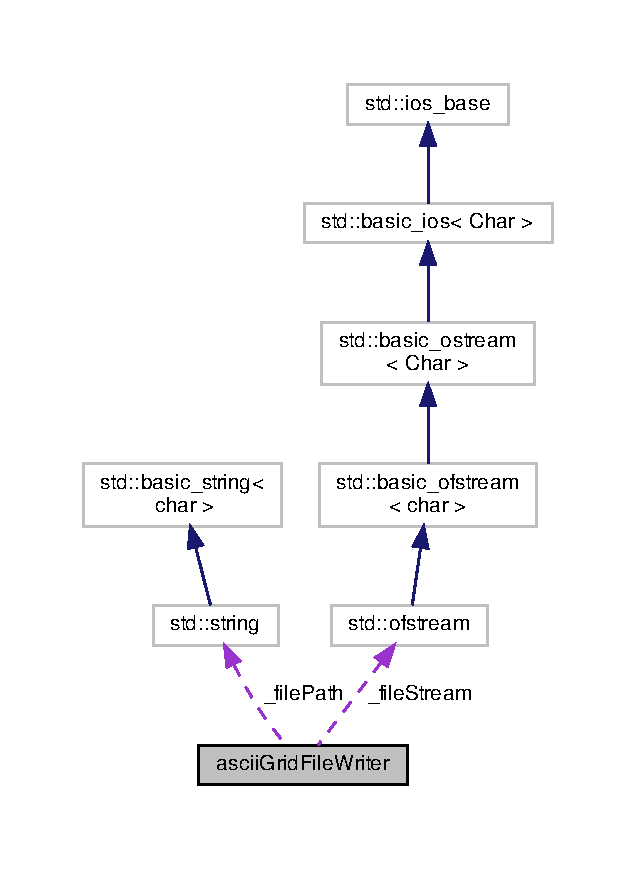
\includegraphics[width=305pt]{classasciiGridFileWriter__coll__graph}
\end{center}
\end{figure}
\subsection*{Public Member Functions}
\begin{DoxyCompactItemize}
\item 
\mbox{\Hypertarget{classasciiGridFileWriter_afeacb4d025b8ec4c81df40267669f393}\label{classasciiGridFileWriter_afeacb4d025b8ec4c81df40267669f393}} 
{\bfseries ascii\+Grid\+File\+Writer} (const std\+::string \&file\+Path, const std\+::string \&file\+Name, unsigned ncols, unsigned nrows, double xllc, double yllc, double cell\+Size, double nodata)
\item 
\mbox{\Hypertarget{classasciiGridFileWriter_aeec3b86649e3f8b0a2ee28bfa9c29790}\label{classasciiGridFileWriter_aeec3b86649e3f8b0a2ee28bfa9c29790}} 
void {\bfseries write\+To\+File} (const std\+::vector$<$ std\+::vector$<$ double $>$$>$ \&)
\item 
\mbox{\Hypertarget{classasciiGridFileWriter_a9194aed7b3c3f7e388db61a1ea057404}\label{classasciiGridFileWriter_a9194aed7b3c3f7e388db61a1ea057404}} 
void {\bfseries write\+Header} (std\+::ofstream \&)
\item 
\mbox{\Hypertarget{classasciiGridFileWriter_ae1ca7a5a88f2d22e577e767c1b7d3c27}\label{classasciiGridFileWriter_ae1ca7a5a88f2d22e577e767c1b7d3c27}} 
void {\bfseries write\+Extra\+Label} (const std\+::string \&)
\end{DoxyCompactItemize}
\subsection*{Private Attributes}
\begin{DoxyCompactItemize}
\item 
\mbox{\Hypertarget{classasciiGridFileWriter_a57fcacc26c1f54f0bd90cacdb61bddba}\label{classasciiGridFileWriter_a57fcacc26c1f54f0bd90cacdb61bddba}} 
unsigned {\bfseries \+\_\+ncols}
\item 
\mbox{\Hypertarget{classasciiGridFileWriter_a7eb307168908d3c54d1b4fd46d5edb37}\label{classasciiGridFileWriter_a7eb307168908d3c54d1b4fd46d5edb37}} 
unsigned {\bfseries \+\_\+nrows}
\item 
\mbox{\Hypertarget{classasciiGridFileWriter_a8f53a9796356585200cc121eb7d4a299}\label{classasciiGridFileWriter_a8f53a9796356585200cc121eb7d4a299}} 
double {\bfseries \+\_\+xllcorner}
\item 
\mbox{\Hypertarget{classasciiGridFileWriter_ad066c235a53a1e2ec52cc6342bd95927}\label{classasciiGridFileWriter_ad066c235a53a1e2ec52cc6342bd95927}} 
double {\bfseries \+\_\+yllcorner}
\item 
\mbox{\Hypertarget{classasciiGridFileWriter_a6ad00d11e5a9bd91d70e905ecf267f67}\label{classasciiGridFileWriter_a6ad00d11e5a9bd91d70e905ecf267f67}} 
double {\bfseries \+\_\+cell\+Size}
\item 
\mbox{\Hypertarget{classasciiGridFileWriter_a218b0e5dfaea479b65366e5031267f6f}\label{classasciiGridFileWriter_a218b0e5dfaea479b65366e5031267f6f}} 
double {\bfseries \+\_\+\+N\+O\+D\+A\+T\+A\+\_\+value}
\item 
\mbox{\Hypertarget{classasciiGridFileWriter_a9aa51246fc6a5d3bb1a92474ae549aeb}\label{classasciiGridFileWriter_a9aa51246fc6a5d3bb1a92474ae549aeb}} 
std\+::ofstream {\bfseries \+\_\+file\+Stream}
\item 
\mbox{\Hypertarget{classasciiGridFileWriter_ad82a8e040c9810ea1bf0b3abfc89689d}\label{classasciiGridFileWriter_ad82a8e040c9810ea1bf0b3abfc89689d}} 
std\+::string {\bfseries \+\_\+file\+Path}
\end{DoxyCompactItemize}


\subsection{Detailed Description}


Definition at line 5 of file ascii\+Grid\+File\+Writer.\+h.



The documentation for this class was generated from the following files\+:\begin{DoxyCompactItemize}
\item 
ascii\+Grid\+File\+Writer.\+h\item 
ascii\+Grid\+File\+Writer.\+cpp\end{DoxyCompactItemize}

\hypertarget{classconfiguration}{}\section{configuration Class Reference}
\label{classconfiguration}\index{configuration@{configuration}}


\subsection{Detailed Description}


Definition at line 8 of file config.\+h.



The documentation for this class was generated from the following file\+:\begin{DoxyCompactItemize}
\item 
config.\+h\end{DoxyCompactItemize}

\hypertarget{classdisease}{}\section{disease Class Reference}
\label{classdisease}\index{disease@{disease}}
\subsection*{Public Member Functions}
\begin{DoxyCompactItemize}
\item 
\mbox{\Hypertarget{classdisease_afb32990aebbbda5e4c768c33863de1ec}\label{classdisease_afb32990aebbbda5e4c768c33863de1ec}} 
{\bfseries disease} (std\+::string)
\item 
\mbox{\Hypertarget{classdisease_a2e43aa4e1b237b34a088142e5ba05645}\label{classdisease_a2e43aa4e1b237b34a088142e5ba05645}} 
void {\bfseries infect} ()
\item 
\mbox{\Hypertarget{classdisease_afea5ed484afbc1c34188041e29b5223f}\label{classdisease_afea5ed484afbc1c34188041e29b5223f}} 
bool {\bfseries infected} ()
\item 
\mbox{\Hypertarget{classdisease_ac806183c372b67568f1cce1f564a7cec}\label{classdisease_ac806183c372b67568f1cce1f564a7cec}} 
bool {\bfseries infectious} ()
\item 
\mbox{\Hypertarget{classdisease_afa1406922bad5c37522a78f4a246d8cf}\label{classdisease_afa1406922bad5c37522a78f4a246d8cf}} 
double {\bfseries infection\+Distance} ()
\item 
\mbox{\Hypertarget{classdisease_a75a1c90ff2112da686cd2e20705238c7}\label{classdisease_a75a1c90ff2112da686cd2e20705238c7}} 
bool {\bfseries maybe\+Become\+Infectious} ()
\item 
\mbox{\Hypertarget{classdisease_ae99ba952f5e81ce98e2d2b849c05ce04}\label{classdisease_ae99ba952f5e81ce98e2d2b849c05ce04}} 
bool {\bfseries infection\+Occurs} ()
\item 
\mbox{\Hypertarget{classdisease_add6e8db6abec70b4bd1eae3e6f2a3cd2}\label{classdisease_add6e8db6abec70b4bd1eae3e6f2a3cd2}} 
bool {\bfseries try\+To\+Recover} ()
\item 
\mbox{\Hypertarget{classdisease_a50f9409e8a2df6eab075b0610ad68114}\label{classdisease_a50f9409e8a2df6eab075b0610ad68114}} 
bool {\bfseries recovered} ()
\item 
\mbox{\Hypertarget{classdisease_aabaa74deee9e5b68062f9b09674c1dc5}\label{classdisease_aabaa74deee9e5b68062f9b09674c1dc5}} 
void {\bfseries update} ()
\item 
\mbox{\Hypertarget{classdisease_aac3946d6d35b4d61163add744e3f1bb9}\label{classdisease_aac3946d6d35b4d61163add744e3f1bb9}} 
bool {\bfseries need\+Hospitalisation} (double \&, const std\+::string \&)
\item 
\mbox{\Hypertarget{classdisease_a4347cb7840d80258b67caa3f169b25e8}\label{classdisease_a4347cb7840d80258b67caa3f169b25e8}} 
bool {\bfseries need\+Critical\+Care} (double \&, const std\+::string \&)
\item 
\mbox{\Hypertarget{classdisease_a4bb1ba1a5fc9af6a941bf690d2ab2908}\label{classdisease_a4bb1ba1a5fc9af6a941bf690d2ab2908}} 
bool {\bfseries critical\+Fatality} (const std\+::string \&)
\end{DoxyCompactItemize}
\subsection*{Static Public Member Functions}
\begin{DoxyCompactItemize}
\item 
\mbox{\Hypertarget{classdisease_a8644518f31d29b005037165360968ecb}\label{classdisease_a8644518f31d29b005037165360968ecb}} 
static void {\bfseries test} ()
\item 
\mbox{\Hypertarget{classdisease_a7ca663d0151be8444ff0c79e0439450e}\label{classdisease_a7ca663d0151be8444ff0c79e0439450e}} 
static void {\bfseries test\+Message} (std\+::string, bool)
\end{DoxyCompactItemize}
\subsection*{Private Member Functions}
\begin{DoxyCompactItemize}
\item 
\mbox{\Hypertarget{classdisease_ac4ba6bb0b1c4d7812623af9e5a1a382b}\label{classdisease_ac4ba6bb0b1c4d7812623af9e5a1a382b}} 
std\+::string {\bfseries get\+Decade} (double \&age)
\end{DoxyCompactItemize}
\subsection*{Private Attributes}
\begin{DoxyCompactItemize}
\item 
\mbox{\Hypertarget{classdisease_ae2e024b1565492d53e22ae853a54076b}\label{classdisease_ae2e024b1565492d53e22ae853a54076b}} 
bool {\bfseries \+\_\+infected}
\item 
\mbox{\Hypertarget{classdisease_a4cef9a43e687cce66a6e083f4cbcc759}\label{classdisease_a4cef9a43e687cce66a6e083f4cbcc759}} 
bool {\bfseries \+\_\+recovered}
\item 
\mbox{\Hypertarget{classdisease_a1c050964c5b68ec72ef15bfd41e45c45}\label{classdisease_a1c050964c5b68ec72ef15bfd41e45c45}} 
bool {\bfseries \+\_\+infectious}
\item 
\mbox{\Hypertarget{classdisease_a9893b408c1f6daccb8a00a07696b45ab}\label{classdisease_a9893b408c1f6daccb8a00a07696b45ab}} 
bool {\bfseries \+\_\+died}
\item 
\mbox{\Hypertarget{classdisease_a5985d317c6b0890c7f99ec71542b3e04}\label{classdisease_a5985d317c6b0890c7f99ec71542b3e04}} 
bool {\bfseries \+\_\+asymptomatic}
\item 
\mbox{\Hypertarget{classdisease_a12c3fe5e2b7973fdab73be57ea35bf02}\label{classdisease_a12c3fe5e2b7973fdab73be57ea35bf02}} 
double {\bfseries \+\_\+infection\+Rate}
\item 
\mbox{\Hypertarget{classdisease_ad023af323ca4a780b6287244f34a6aaa}\label{classdisease_ad023af323ca4a780b6287244f34a6aaa}} 
double {\bfseries \+\_\+recovery\+Time}
\item 
\mbox{\Hypertarget{classdisease_a4e074e57f0b2c8c4b8a6534f5801c426}\label{classdisease_a4e074e57f0b2c8c4b8a6534f5801c426}} 
double {\bfseries \+\_\+latency\+Time}
\item 
\mbox{\Hypertarget{classdisease_a72c1334514dc57ac05849ece61ee183d}\label{classdisease_a72c1334514dc57ac05849ece61ee183d}} 
double {\bfseries \+\_\+infection\+Distance}
\item 
\mbox{\Hypertarget{classdisease_a567c5cc74c752810c746800ab6df53ae}\label{classdisease_a567c5cc74c752810c746800ab6df53ae}} 
unsigned {\bfseries \+\_\+timer}
\end{DoxyCompactItemize}


\subsection{Detailed Description}


Definition at line 11 of file disease.\+h.



The documentation for this class was generated from the following files\+:\begin{DoxyCompactItemize}
\item 
disease.\+h\item 
disease.\+cpp\end{DoxyCompactItemize}

\hypertarget{structevent}{}\section{event Struct Reference}
\label{structevent}\index{event@{event}}


Collaboration diagram for event\+:
\nopagebreak
\begin{figure}[H]
\begin{center}
\leavevmode
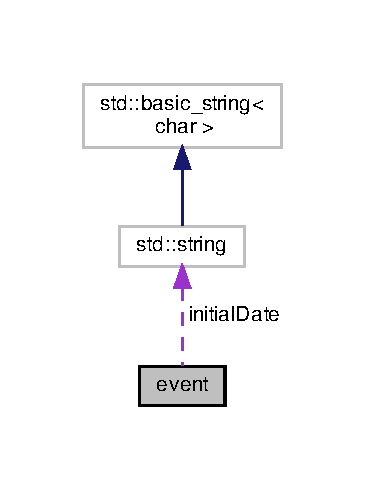
\includegraphics[width=176pt]{structevent__coll__graph}
\end{center}
\end{figure}
\subsection*{Public Member Functions}
\begin{DoxyCompactItemize}
\item 
\mbox{\Hypertarget{structevent_a730f8d0598f47a0991bf1e4148435b2d}\label{structevent_a730f8d0598f47a0991bf1e4148435b2d}} 
{\bfseries event} (string s, unsigned p)
\item 
\mbox{\Hypertarget{structevent_a4f61b72722376cd96b7e04218144acbf}\label{structevent_a4f61b72722376cd96b7e04218144acbf}} 
{\bfseries event} (ptime t, unsigned p)
\item 
\mbox{\Hypertarget{structevent_a8db259e5b385cc72d89aec4a32696f7b}\label{structevent_a8db259e5b385cc72d89aec4a32696f7b}} 
{\bfseries event} (const \mbox{\hyperlink{structevent}{event}} \&e)
\item 
\mbox{\Hypertarget{structevent_abbe5e998115b21515138c27e290e3110}\label{structevent_abbe5e998115b21515138c27e290e3110}} 
void {\bfseries set\+End\+Time} (string s)
\item 
\mbox{\Hypertarget{structevent_ab21a6b2eea8829fd6d7ed60868472d1f}\label{structevent_ab21a6b2eea8829fd6d7ed60868472d1f}} 
void {\bfseries add\+Days\+To\+End\+Time} (int d)
\item 
\mbox{\Hypertarget{structevent_a0cb1cccaf2a6e06ad214ce66ae06befb}\label{structevent_a0cb1cccaf2a6e06ad214ce66ae06befb}} 
void {\bfseries add\+Minutes\+To\+End\+Time} (int m)
\item 
\mbox{\Hypertarget{structevent_a1f28e916e6863e303f60802e951fb37f}\label{structevent_a1f28e916e6863e303f60802e951fb37f}} 
void {\bfseries add\+Seconds\+To\+End\+Time} (int s)
\end{DoxyCompactItemize}
\subsection*{Public Attributes}
\begin{DoxyCompactItemize}
\item 
\mbox{\Hypertarget{structevent_aeb16a5736888611f5424e5da280b5cbd}\label{structevent_aeb16a5736888611f5424e5da280b5cbd}} 
unsigned {\bfseries tick}
\item 
\mbox{\Hypertarget{structevent_a763d19924574b410961a3423385f110a}\label{structevent_a763d19924574b410961a3423385f110a}} 
ptime {\bfseries end\+Time}
\item 
\mbox{\Hypertarget{structevent_aa85754648c3695f2284ed9c2ac726d33}\label{structevent_aa85754648c3695f2284ed9c2ac726d33}} 
string {\bfseries initial\+Date}
\item 
\mbox{\Hypertarget{structevent_ae963ec1a3906a288458ce5f754d17482}\label{structevent_ae963ec1a3906a288458ce5f754d17482}} 
unsigned {\bfseries place}
\end{DoxyCompactItemize}


\subsection{Detailed Description}


Definition at line 6 of file timetable.\+h.



The documentation for this struct was generated from the following file\+:\begin{DoxyCompactItemize}
\item 
timetable.\+h\end{DoxyCompactItemize}

\hypertarget{classextent3D}{}\section{extent3D Class Reference}
\label{classextent3D}\index{extent3D@{extent3D}}
\subsection*{Public Member Functions}
\begin{DoxyCompactItemize}
\item 
\mbox{\Hypertarget{classextent3D_a4c7d9d3faf289b7d2fcebdb3e6a059d9}\label{classextent3D_a4c7d9d3faf289b7d2fcebdb3e6a059d9}} 
{\bfseries extent3D} (double x\+\_\+, double y\+\_\+, double z\+\_\+)
\item 
\mbox{\Hypertarget{classextent3D_af984e85893bed0ffd4e1ee406bf7580c}\label{classextent3D_af984e85893bed0ffd4e1ee406bf7580c}} 
void {\bfseries set\+Extent} (double x\+\_\+, double y\+\_\+, double z\+\_\+)
\item 
\mbox{\Hypertarget{classextent3D_aeaca37d620d74a00632f486cbb1c818e}\label{classextent3D_aeaca37d620d74a00632f486cbb1c818e}} 
double {\bfseries get\+Size} ()
\end{DoxyCompactItemize}
\subsection*{Public Attributes}
\begin{DoxyCompactItemize}
\item 
\mbox{\Hypertarget{classextent3D_ae32558ee0b7cbb81740178295cd0925a}\label{classextent3D_ae32558ee0b7cbb81740178295cd0925a}} 
double {\bfseries x}
\item 
\mbox{\Hypertarget{classextent3D_af38c998f1c089e645befc1c82b39ca32}\label{classextent3D_af38c998f1c089e645befc1c82b39ca32}} 
double {\bfseries y}
\item 
\mbox{\Hypertarget{classextent3D_a8849ee5b9cfcb0662d6ff841157e94a5}\label{classextent3D_a8849ee5b9cfcb0662d6ff841157e94a5}} 
double {\bfseries z}
\end{DoxyCompactItemize}


\subsection{Detailed Description}


Definition at line 4 of file layer.\+h.



The documentation for this class was generated from the following file\+:\begin{DoxyCompactItemize}
\item 
layer.\+h\end{DoxyCompactItemize}

\hypertarget{classfancyWorldpopFactory}{}\section{fancy\+Worldpop\+Factory Class Reference}
\label{classfancyWorldpopFactory}\index{fancy\+Worldpop\+Factory@{fancy\+Worldpop\+Factory}}


Inheritance diagram for fancy\+Worldpop\+Factory\+:\nopagebreak
\begin{figure}[H]
\begin{center}
\leavevmode
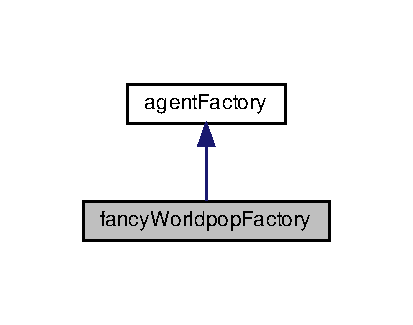
\includegraphics[width=198pt]{classfancyWorldpopFactory__inherit__graph}
\end{center}
\end{figure}


Collaboration diagram for fancy\+Worldpop\+Factory\+:\nopagebreak
\begin{figure}[H]
\begin{center}
\leavevmode
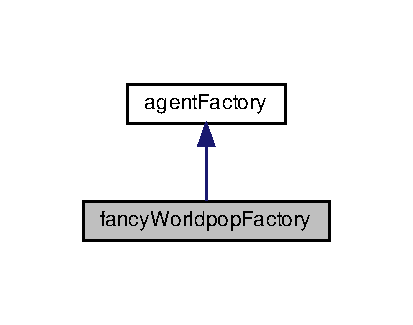
\includegraphics[width=198pt]{classfancyWorldpopFactory__coll__graph}
\end{center}
\end{figure}
\subsection*{Private Member Functions}
\begin{DoxyCompactItemize}
\item 
\mbox{\Hypertarget{classfancyWorldpopFactory_a02ec5ffbb45ff8975f6e142dcd4520e3}\label{classfancyWorldpopFactory_a02ec5ffbb45ff8975f6e142dcd4520e3}} 
void {\bfseries create\+Agents} (vector$<$ \mbox{\hyperlink{classagent}{agent}} $\ast$$>$ \&\mbox{\hyperlink{classagents}{agents}})
\end{DoxyCompactItemize}
\subsection*{Additional Inherited Members}


\subsection{Detailed Description}


Definition at line 15 of file agent\+Factory.\+h.



The documentation for this class was generated from the following file\+:\begin{DoxyCompactItemize}
\item 
agent\+Factory.\+h\end{DoxyCompactItemize}

\hypertarget{classlayer}{}\section{layer Class Reference}
\label{classlayer}\index{layer@{layer}}


Inheritance diagram for layer\+:
\nopagebreak
\begin{figure}[H]
\begin{center}
\leavevmode
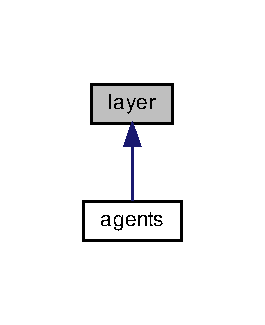
\includegraphics[width=127pt]{classlayer__inherit__graph}
\end{center}
\end{figure}


Collaboration diagram for layer\+:
\nopagebreak
\begin{figure}[H]
\begin{center}
\leavevmode
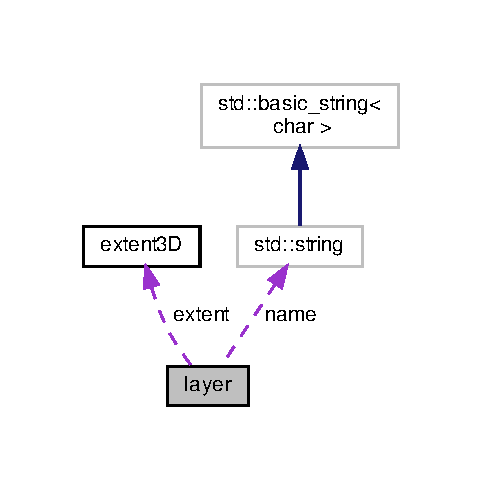
\includegraphics[width=232pt]{classlayer__coll__graph}
\end{center}
\end{figure}
\subsection*{Public Member Functions}
\begin{DoxyCompactItemize}
\item 
\mbox{\Hypertarget{classlayer_ad153d45a8b34da24fa84f83dd828b960}\label{classlayer_ad153d45a8b34da24fa84f83dd828b960}} 
virtual bool {\bfseries update} ()
\item 
\mbox{\Hypertarget{classlayer_a57de706157ab0ec174e0619e7829f6e9}\label{classlayer_a57de706157ab0ec174e0619e7829f6e9}} 
virtual \mbox{\hyperlink{classextent3D}{extent3D}} {\bfseries get\+Extent} ()
\item 
\mbox{\Hypertarget{classlayer_a965efdddf4b7e7bd2344c24689eb48f9}\label{classlayer_a965efdddf4b7e7bd2344c24689eb48f9}} 
virtual void {\bfseries set\+Extent} (double, double, double)
\item 
\mbox{\Hypertarget{classlayer_a0757a4ef63be3d92e5a22139533daaab}\label{classlayer_a0757a4ef63be3d92e5a22139533daaab}} 
virtual double {\bfseries get\+Size} ()
\item 
\mbox{\Hypertarget{classlayer_a40931bf282a03bf88fc002954b496414}\label{classlayer_a40931bf282a03bf88fc002954b496414}} 
void {\bfseries set\+Name} (std\+::string)
\end{DoxyCompactItemize}
\subsection*{Protected Attributes}
\begin{DoxyCompactItemize}
\item 
\mbox{\Hypertarget{classlayer_a9233a262fa15466db3e2e1c2b422469a}\label{classlayer_a9233a262fa15466db3e2e1c2b422469a}} 
std\+::string {\bfseries name}
\item 
\mbox{\Hypertarget{classlayer_ac80253765b74a00ad838fa3eb9c5724d}\label{classlayer_ac80253765b74a00ad838fa3eb9c5724d}} 
\mbox{\hyperlink{classextent3D}{extent3D}} {\bfseries extent}
\end{DoxyCompactItemize}


\subsection{Detailed Description}


Definition at line 13 of file layer.\+h.



The documentation for this class was generated from the following files\+:\begin{DoxyCompactItemize}
\item 
layer.\+h\item 
layer.\+cpp\end{DoxyCompactItemize}

\hypertarget{classmodel}{}\section{model Class Reference}
\label{classmodel}\index{model@{model}}


The model holds the agents in a vector and drives their updates.  




{\ttfamily \#include $<$model.\+h$>$}



Collaboration diagram for model\+:\nopagebreak
\begin{figure}[H]
\begin{center}
\leavevmode
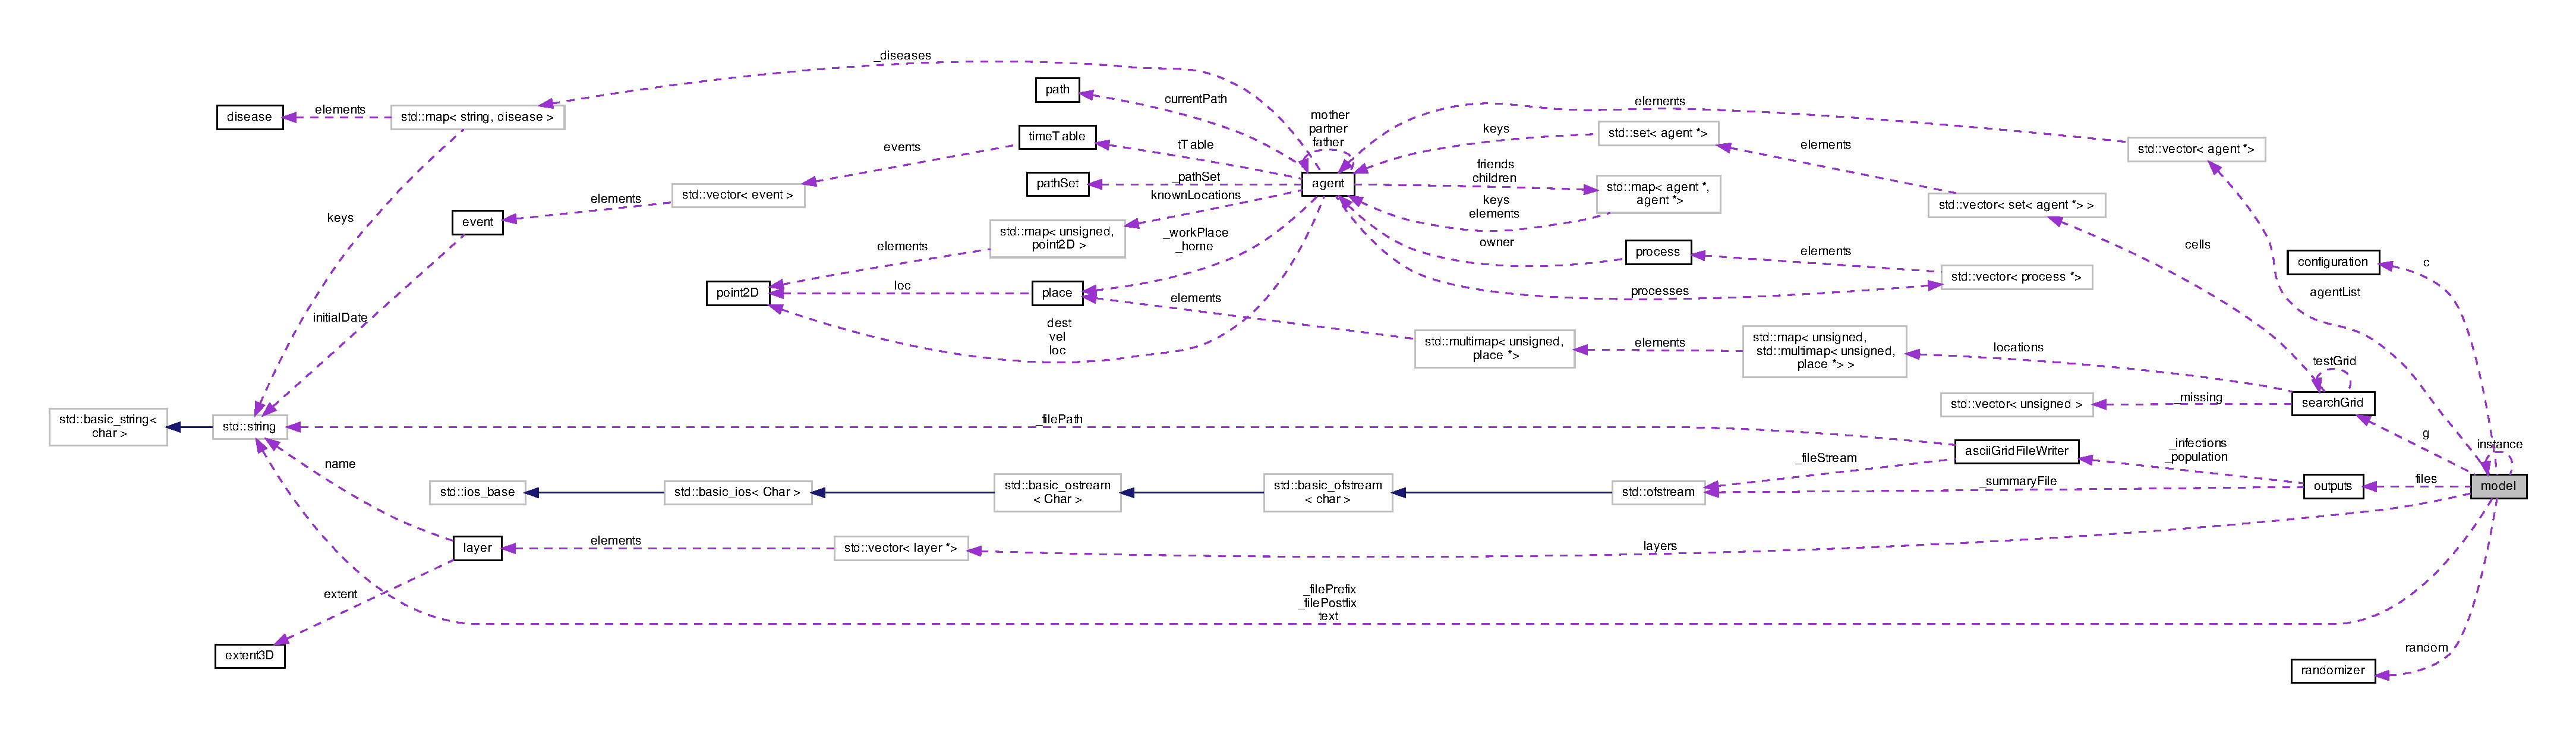
\includegraphics[width=350pt]{classmodel__coll__graph}
\end{center}
\end{figure}
\subsection*{Public Member Functions}
\begin{DoxyCompactItemize}
\item 
\mbox{\Hypertarget{classmodel_abd493c0d266874a1913cccc99918ac62}\label{classmodel_abd493c0d266874a1913cccc99918ac62}} 
void {\bfseries init} ()
\item 
\mbox{\Hypertarget{classmodel_a7fc3b1ce57ed26472e3bfbe10a655659}\label{classmodel_a7fc3b1ce57ed26472e3bfbe10a655659}} 
bool {\bfseries update} ()
\item 
\mbox{\Hypertarget{classmodel_a477cd70af36d7f510e98d26fb9f25c07}\label{classmodel_a477cd70af36d7f510e98d26fb9f25c07}} 
void {\bfseries run\+One\+Step} ()
\item 
\mbox{\Hypertarget{classmodel_a01ccb636491164b70ec3c015e12de80d}\label{classmodel_a01ccb636491164b70ec3c015e12de80d}} 
void {\bfseries run} ()
\item 
\mbox{\Hypertarget{classmodel_abae5132b97a5b93af153ae0756813200}\label{classmodel_abae5132b97a5b93af153ae0756813200}} 
void {\bfseries run\+Up\+To} (long n)
\item 
\mbox{\Hypertarget{classmodel_a8f54f46930b3b3af375c0cdd1abfcbba}\label{classmodel_a8f54f46930b3b3af375c0cdd1abfcbba}} 
std\+::string {\bfseries filepath} ()
\item 
\mbox{\Hypertarget{classmodel_a674f58eb59ee2fd722291879557b5343}\label{classmodel_a674f58eb59ee2fd722291879557b5343}} 
void {\bfseries add} (\mbox{\hyperlink{classlayer}{layer}} $\ast$l)
\item 
\mbox{\Hypertarget{classmodel_a1cf467caa1e2e1cd36ce6b609d74a703}\label{classmodel_a1cf467caa1e2e1cd36ce6b609d74a703}} 
\mbox{\hyperlink{classlayer}{layer}} $\ast$ {\bfseries get\+Layer} (unsigned)
\item 
\mbox{\Hypertarget{classmodel_aa778b767859473ccb2b2d3268bc23d23}\label{classmodel_aa778b767859473ccb2b2d3268bc23d23}} 
void {\bfseries finish} ()
\item 
\mbox{\Hypertarget{classmodel_a24fd9c8535250831cd798d9594e1a072}\label{classmodel_a24fd9c8535250831cd798d9594e1a072}} 
double {\bfseries get\+Size} ()
\item 
\mbox{\Hypertarget{classmodel_a6895d06ffc6a5447836b0ca84f544a33}\label{classmodel_a6895d06ffc6a5447836b0ca84f544a33}} 
string {\bfseries get\+Text} ()
\end{DoxyCompactItemize}
\subsection*{Static Public Member Functions}
\begin{DoxyCompactItemize}
\item 
\mbox{\Hypertarget{classmodel_a89a557ca7e1fe3ad432092b29a87b459}\label{classmodel_a89a557ca7e1fe3ad432092b29a87b459}} 
static \mbox{\hyperlink{classmodel}{model}} \& {\bfseries get\+Instance} ()
\end{DoxyCompactItemize}
\subsection*{Public Attributes}
\begin{DoxyCompactItemize}
\item 
\mbox{\Hypertarget{classmodel_a98fc532cc6ca8ec05f9ca7885f8310a6}\label{classmodel_a98fc532cc6ca8ec05f9ca7885f8310a6}} 
unsigned {\bfseries tick}
\item 
\mbox{\Hypertarget{classmodel_acea5467698b2a0bf754cb2680e292959}\label{classmodel_acea5467698b2a0bf754cb2680e292959}} 
float {\bfseries dt}
\item 
\mbox{\Hypertarget{classmodel_ae2282007872b337492343762def0693c}\label{classmodel_ae2282007872b337492343762def0693c}} 
\mbox{\hyperlink{classsearchGrid}{search\+Grid}} {\bfseries g}
\item 
\mbox{\Hypertarget{classmodel_a72a2d5ccc0f9248e52e5baada92f3c65}\label{classmodel_a72a2d5ccc0f9248e52e5baada92f3c65}} 
vector$<$ \mbox{\hyperlink{classagent}{agent}} $\ast$ $>$ $\ast$ {\bfseries agent\+List}
\item 
\mbox{\Hypertarget{classmodel_a83b015b77324bc70fb2a74ef90885291}\label{classmodel_a83b015b77324bc70fb2a74ef90885291}} 
\mbox{\hyperlink{classrandomizer}{randomizer}} {\bfseries random}
\end{DoxyCompactItemize}
\subsection*{Private Member Functions}
\begin{DoxyCompactItemize}
\item 
\mbox{\Hypertarget{classmodel_aa82375be2bd53080d3a5e3fcfa0df30c}\label{classmodel_aa82375be2bd53080d3a5e3fcfa0df30c}} 
void {\bfseries clean} ()
\item 
\mbox{\Hypertarget{classmodel_af6e1bf4eb735c76eb9f77a10b0a64ff8}\label{classmodel_af6e1bf4eb735c76eb9f77a10b0a64ff8}} 
void {\bfseries set\+Output\+File\+Paths} ()
\end{DoxyCompactItemize}
\subsection*{Private Attributes}
\begin{DoxyCompactItemize}
\item 
\mbox{\Hypertarget{classmodel_ac3dcc51c9ff2eecdd10793629206b65d}\label{classmodel_ac3dcc51c9ff2eecdd10793629206b65d}} 
vector$<$ \mbox{\hyperlink{classlayer}{layer}} $\ast$ $>$ {\bfseries layers}
\item 
\mbox{\Hypertarget{classmodel_a742b5b77848d0dbdc032e1a51274ba08}\label{classmodel_a742b5b77848d0dbdc032e1a51274ba08}} 
\mbox{\hyperlink{classconfiguration}{configuration}} $\ast$ {\bfseries c}
\item 
\mbox{\Hypertarget{classmodel_a3791961971c5e979086eadc7127e7c78}\label{classmodel_a3791961971c5e979086eadc7127e7c78}} 
string {\bfseries text}
\item 
\mbox{\Hypertarget{classmodel_a8eae0977871b806881319ff8091f5389}\label{classmodel_a8eae0977871b806881319ff8091f5389}} 
\mbox{\hyperlink{classoutputs}{outputs}} $\ast$ {\bfseries files}
\item 
\mbox{\Hypertarget{classmodel_a361a901c3aa70774e254457065ebeb0e}\label{classmodel_a361a901c3aa70774e254457065ebeb0e}} 
std\+::string {\bfseries \+\_\+file\+Prefix}
\item 
\mbox{\Hypertarget{classmodel_ae5e7e93a6aeb1584eda754f91b1cdd4e}\label{classmodel_ae5e7e93a6aeb1584eda754f91b1cdd4e}} 
std\+::string {\bfseries \+\_\+file\+Postfix}
\end{DoxyCompactItemize}
\subsection*{Static Private Attributes}
\begin{DoxyCompactItemize}
\item 
\mbox{\Hypertarget{classmodel_a486d4ee9311769407729f640fe3f42b4}\label{classmodel_a486d4ee9311769407729f640fe3f42b4}} 
static \mbox{\hyperlink{classmodel}{model}} $\ast$ {\bfseries instance} =N\+U\+LL
\end{DoxyCompactItemize}


\subsection{Detailed Description}
The model holds the agents in a vector and drives their updates. 

This class is a singleton (see e.\+g Shalloway and Trott \char`\"{}\+Design Patterns Explained\char`\"{}) -\/ only one instance of the class can be created on any thread. The class has a protected constructor so that no instance can be created directly -\/ instead the static function get\+Instance() must be used. The first time get\+Instance() is called, the class constructor is used to generate the required data -\/ thereafter the constructor is not called again, and get\+Instance returns a pointer to the pre-\/existing instance. This means get\+Instance() can be called anywhere within the code and it will return the same environmental information~\newline
The init funtion should be called after first creation of the singleton for those items that depend on a fully completed singleton for their existence e.\+g. the configuration class, which calls model\+::add(layer$\ast$) usage example\+:-\/~\newline

\begin{DoxyCode}
\mbox{\hyperlink{classmodel}{model}}* m=model::getInstance();
m->init();
\textcolor{comment}{//advance to the next state}
m->update();
\end{DoxyCode}


\begin{DoxyAuthor}{Author}
Mike Bithell \href{mailto:mb425@cam.ac.uk}{\tt mb425@cam.\+ac.\+uk} 
\end{DoxyAuthor}


Definition at line 59 of file model.\+h.



The documentation for this class was generated from the following files\+:\begin{DoxyCompactItemize}
\item 
\mbox{\hyperlink{model_8h}{model.\+h}}\item 
\mbox{\hyperlink{model_8cpp}{model.\+cpp}}\end{DoxyCompactItemize}

\hypertarget{classmovement}{}\section{movement Class Reference}
\label{classmovement}\index{movement@{movement}}


Inheritance diagram for movement\+:
\nopagebreak
\begin{figure}[H]
\begin{center}
\leavevmode
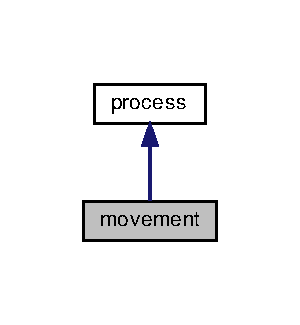
\includegraphics[width=144pt]{classmovement__inherit__graph}
\end{center}
\end{figure}


Collaboration diagram for movement\+:
\nopagebreak
\begin{figure}[H]
\begin{center}
\leavevmode
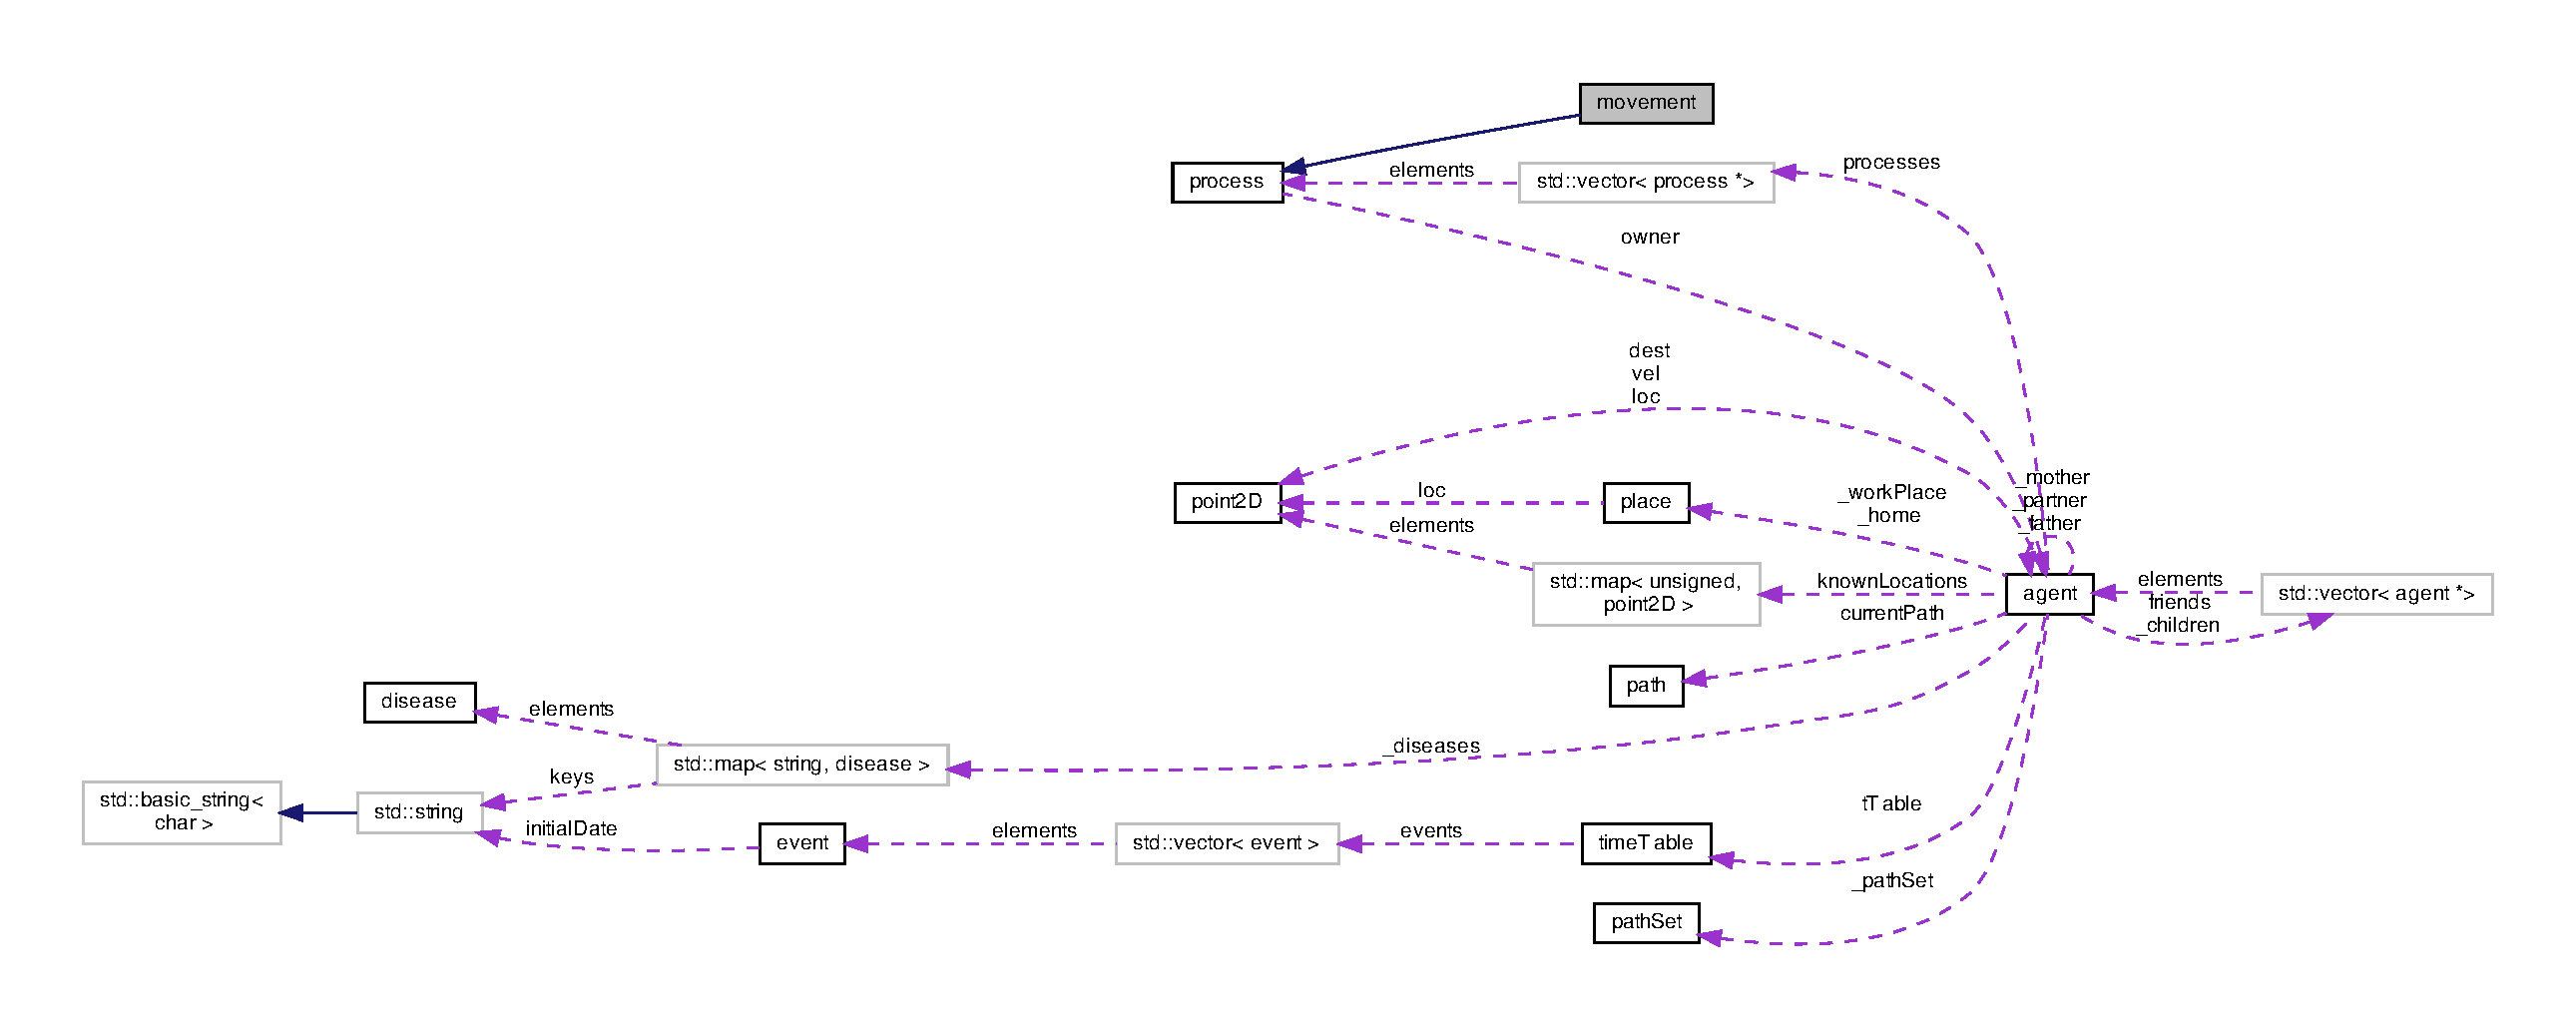
\includegraphics[width=350pt]{classmovement__coll__graph}
\end{center}
\end{figure}
\subsection*{Public Member Functions}
\begin{DoxyCompactItemize}
\item 
\mbox{\Hypertarget{classmovement_aed3c0d8fffab4ddfcf671869eb3167fd}\label{classmovement_aed3c0d8fffab4ddfcf671869eb3167fd}} 
{\bfseries movement} (\mbox{\hyperlink{classagent}{agent}} $\ast$a)
\item 
\mbox{\Hypertarget{classmovement_aad069c445064e63352ae38b00deec2a9}\label{classmovement_aad069c445064e63352ae38b00deec2a9}} 
void {\bfseries pre\+Update} ()
\item 
\mbox{\Hypertarget{classmovement_affebcf78f2f1f085a8daae74f699a132}\label{classmovement_affebcf78f2f1f085a8daae74f699a132}} 
void {\bfseries update} ()
\item 
\mbox{\Hypertarget{classmovement_a2b5e033ddb01a6df13826d9e3f2b253c}\label{classmovement_a2b5e033ddb01a6df13826d9e3f2b253c}} 
void {\bfseries apply\+Update} ()
\end{DoxyCompactItemize}
\subsection*{Public Attributes}
\begin{DoxyCompactItemize}
\item 
\mbox{\Hypertarget{classmovement_a1d4a21441baf4f59ceabb25e01957197}\label{classmovement_a1d4a21441baf4f59ceabb25e01957197}} 
double {\bfseries xdel}
\item 
\mbox{\Hypertarget{classmovement_a8135db424da53103c601fbe265c4078e}\label{classmovement_a8135db424da53103c601fbe265c4078e}} 
double {\bfseries ydel}
\item 
\mbox{\Hypertarget{classmovement_a2ad6baf5e20f1b04169c355a3eaa7f4a}\label{classmovement_a2ad6baf5e20f1b04169c355a3eaa7f4a}} 
double {\bfseries dvx}
\item 
\mbox{\Hypertarget{classmovement_a14589ed0161d8d248e53421af0e282f8}\label{classmovement_a14589ed0161d8d248e53421af0e282f8}} 
double {\bfseries dvy}
\item 
\mbox{\Hypertarget{classmovement_acf8298233464d137777e8bf3c26a63b2}\label{classmovement_acf8298233464d137777e8bf3c26a63b2}} 
double {\bfseries vdesired}
\item 
\mbox{\Hypertarget{classmovement_aae56090ba1816d74c0a82840e5ee9713}\label{classmovement_aae56090ba1816d74c0a82840e5ee9713}} 
double {\bfseries vmax}
\item 
\mbox{\Hypertarget{classmovement_a6b3db78fd7a26da3a9e6be691902525a}\label{classmovement_a6b3db78fd7a26da3a9e6be691902525a}} 
double {\bfseries vwalk}
\item 
\mbox{\Hypertarget{classmovement_a51035f46709076cf35eb010ba4ba135f}\label{classmovement_a51035f46709076cf35eb010ba4ba135f}} 
double {\bfseries trelax}
\item 
\mbox{\Hypertarget{classmovement_a959ef2b033665694fec3aec1b190b350}\label{classmovement_a959ef2b033665694fec3aec1b190b350}} 
double {\bfseries random\+Wobble}
\end{DoxyCompactItemize}


\subsection{Detailed Description}


Definition at line 6 of file movement.\+h.



The documentation for this class was generated from the following files\+:\begin{DoxyCompactItemize}
\item 
movement.\+h\item 
movement.\+cpp\end{DoxyCompactItemize}

\hypertarget{classoutputs}{}\section{outputs Class Reference}
\label{classoutputs}\index{outputs@{outputs}}


Collaboration diagram for outputs\+:\nopagebreak
\begin{figure}[H]
\begin{center}
\leavevmode
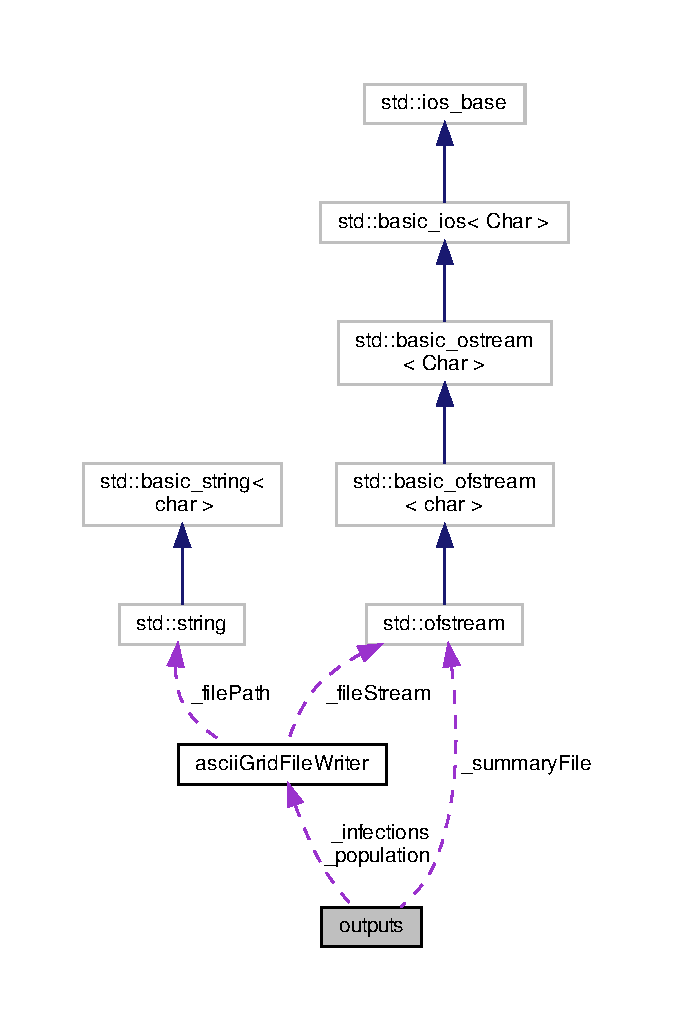
\includegraphics[width=326pt]{classoutputs__coll__graph}
\end{center}
\end{figure}
\subsection*{Public Member Functions}
\begin{DoxyCompactItemize}
\item 
\mbox{\Hypertarget{classoutputs_a84e606322d80c26a9afd60f25d3d9fba}\label{classoutputs_a84e606322d80c26a9afd60f25d3d9fba}} 
void {\bfseries write\+All} ()
\item 
\mbox{\Hypertarget{classoutputs_aca2eded868d51846d8521ea6534bd227}\label{classoutputs_aca2eded868d51846d8521ea6534bd227}} 
void {\bfseries test} ()
\end{DoxyCompactItemize}
\subsection*{Private Attributes}
\begin{DoxyCompactItemize}
\item 
\mbox{\Hypertarget{classoutputs_a8709cb5dd3d58f640cb7194c85b50a18}\label{classoutputs_a8709cb5dd3d58f640cb7194c85b50a18}} 
\mbox{\hyperlink{classasciiGridFileWriter}{ascii\+Grid\+File\+Writer}} $\ast$ {\bfseries \+\_\+infections}
\item 
\mbox{\Hypertarget{classoutputs_aac86ef701212c43f126fde0a5755109b}\label{classoutputs_aac86ef701212c43f126fde0a5755109b}} 
\mbox{\hyperlink{classasciiGridFileWriter}{ascii\+Grid\+File\+Writer}} $\ast$ {\bfseries \+\_\+population}
\item 
\mbox{\Hypertarget{classoutputs_a3a31a7714910a5278a6a5b00df1d0499}\label{classoutputs_a3a31a7714910a5278a6a5b00df1d0499}} 
std\+::ofstream {\bfseries \+\_\+summary\+File}
\item 
\mbox{\Hypertarget{classoutputs_aafdf08a7e20b742367f48fb1cdbc74b8}\label{classoutputs_aafdf08a7e20b742367f48fb1cdbc74b8}} 
double {\bfseries \+\_\+output\+Cell\+Size}
\end{DoxyCompactItemize}


\subsection{Detailed Description}


Definition at line 6 of file outputs.\+h.



The documentation for this class was generated from the following files\+:\begin{DoxyCompactItemize}
\item 
outputs.\+h\item 
outputs.\+cpp\end{DoxyCompactItemize}

\hypertarget{classparameters}{}\section{parameters Class Reference}
\label{classparameters}\index{parameters@{parameters}}


Collaboration diagram for parameters\+:
\nopagebreak
\begin{figure}[H]
\begin{center}
\leavevmode
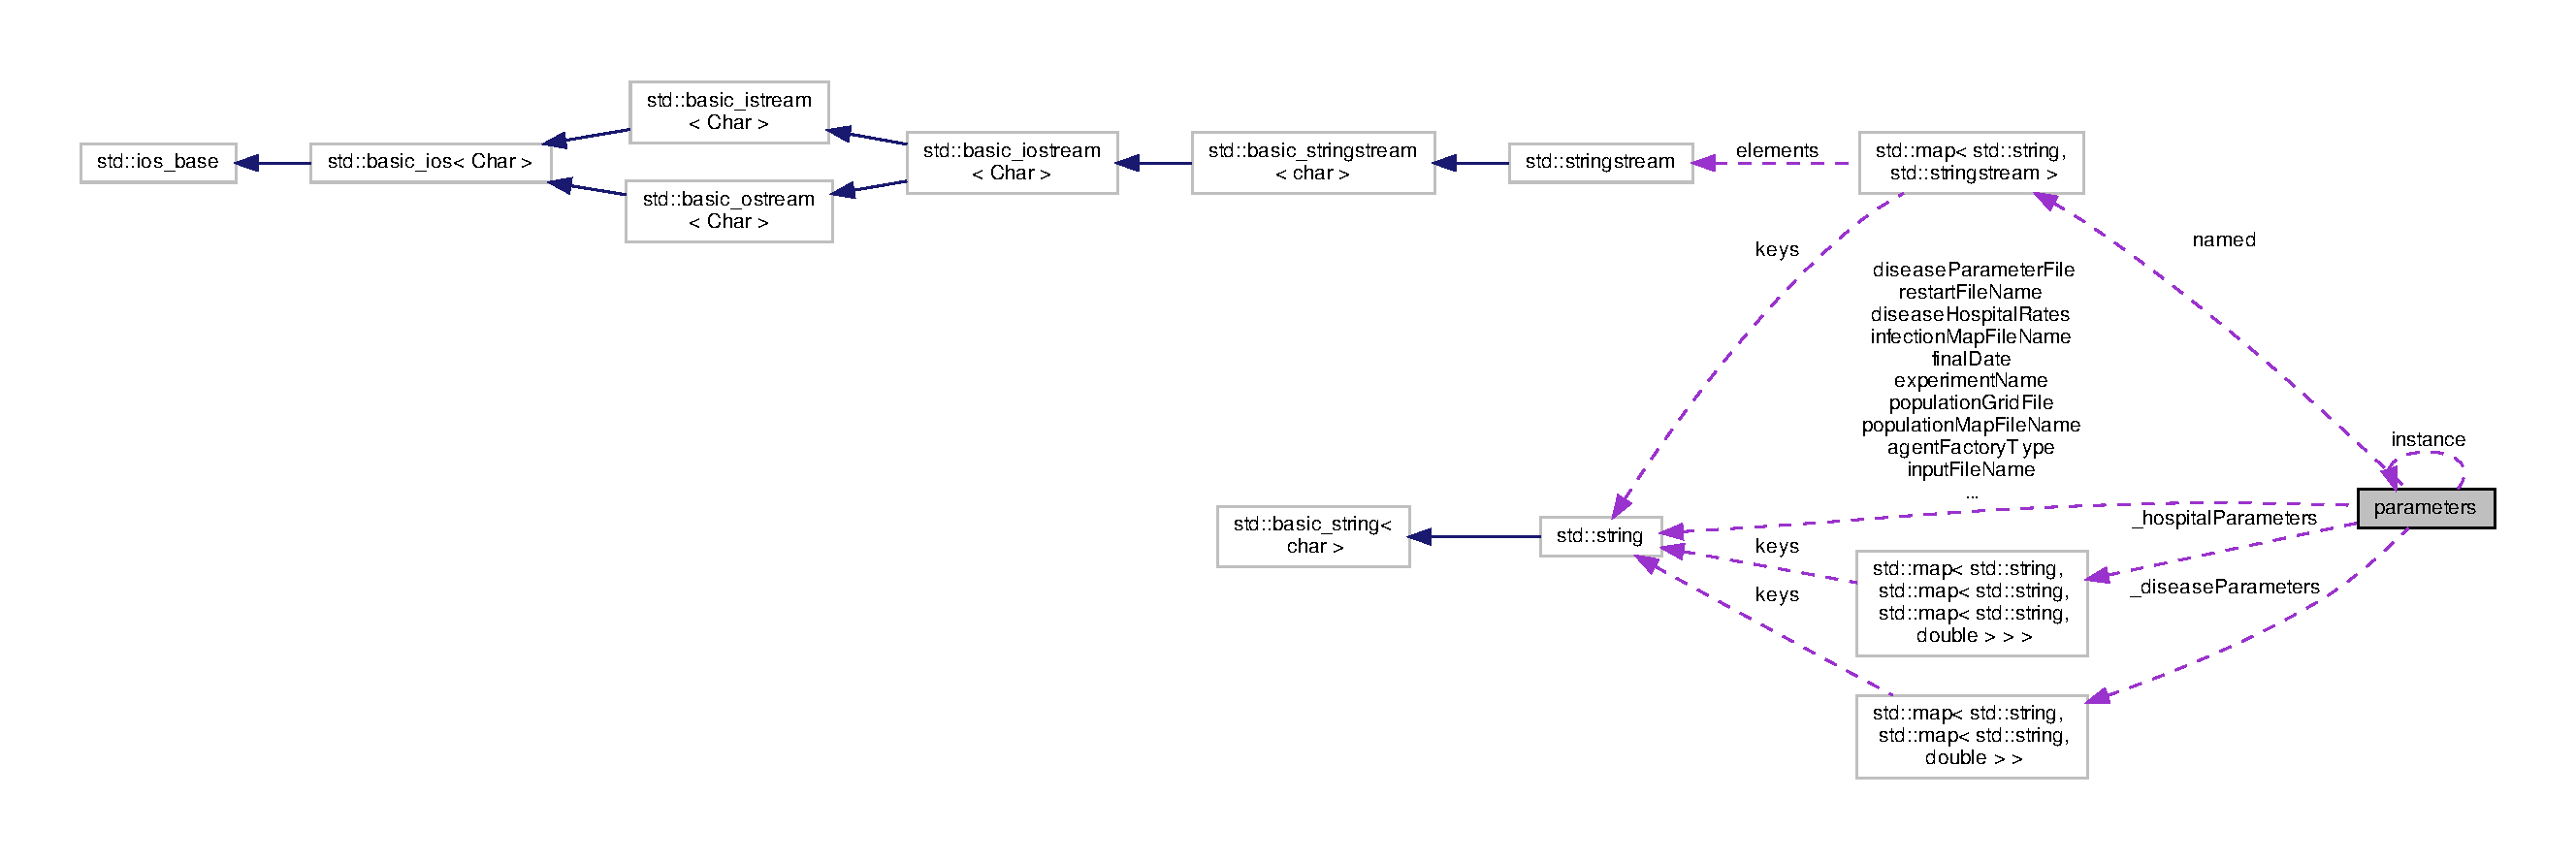
\includegraphics[width=350pt]{classparameters__coll__graph}
\end{center}
\end{figure}
\subsection*{Public Member Functions}
\begin{DoxyCompactItemize}
\item 
\mbox{\Hypertarget{classparameters_a5afb6f0a6eeec826d39795add97c2891}\label{classparameters_a5afb6f0a6eeec826d39795add97c2891}} 
void {\bfseries print\+Parameters} ()
\item 
\mbox{\Hypertarget{classparameters_a1f9a3b98c893d21631f9611202ba4ad6}\label{classparameters_a1f9a3b98c893d21631f9611202ba4ad6}} 
void {\bfseries save\+Parameters} ()
\item 
\mbox{\Hypertarget{classparameters_a62f7b648c3c5c5b71894cdb9825ec5ed}\label{classparameters_a62f7b648c3c5c5b71894cdb9825ec5ed}} 
void {\bfseries get\+Parameters} ()
\item 
\mbox{\Hypertarget{classparameters_a3c25eaa213291dce9de11ace386770a5}\label{classparameters_a3c25eaa213291dce9de11ace386770a5}} 
void {\bfseries read\+Disease\+Parameters} ()
\item 
\mbox{\Hypertarget{classparameters_a29ec80156af04d3729397f122717e4df}\label{classparameters_a29ec80156af04d3729397f122717e4df}} 
double {\bfseries disease} (const std\+::string \&, const std\+::string \&)
\item 
\mbox{\Hypertarget{classparameters_a44a495028fba207fe2de8b2a4d3cae61}\label{classparameters_a44a495028fba207fe2de8b2a4d3cae61}} 
double {\bfseries needs\+Care} (const std\+::string \&, const std\+::string \&, const std\+::string \&)
\item 
\mbox{\Hypertarget{classparameters_ac12f6a6ab14a6f5ce5f48e4c535f3e03}\label{classparameters_ac12f6a6ab14a6f5ce5f48e4c535f3e03}} 
void {\bfseries set\+Run\+Number} (std\+::string n)
\end{DoxyCompactItemize}
\subsection*{Static Public Member Functions}
\begin{DoxyCompactItemize}
\item 
\mbox{\Hypertarget{classparameters_afd0f251397ef8deef8bbb63c7d86bebb}\label{classparameters_afd0f251397ef8deef8bbb63c7d86bebb}} 
static \mbox{\hyperlink{classparameters}{parameters}} \& {\bfseries get\+Instance} ()
\item 
\mbox{\Hypertarget{classparameters_aec2cc19583134030d567ea02455adf8a}\label{classparameters_aec2cc19583134030d567ea02455adf8a}} 
static \mbox{\hyperlink{classparameters}{parameters}} \& {\bfseries get\+Instance} (string)
\end{DoxyCompactItemize}
\subsection*{Public Attributes}
\begin{DoxyCompactItemize}
\item 
\mbox{\Hypertarget{classparameters_a4684bd411109daec28b803323a6452db}\label{classparameters_a4684bd411109daec28b803323a6452db}} 
double {\bfseries time\+Step}
\item 
\mbox{\Hypertarget{classparameters_a7947c3c95a18fc3b979e14251c40574c}\label{classparameters_a7947c3c95a18fc3b979e14251c40574c}} 
int {\bfseries random\+Seed}
\item 
\mbox{\Hypertarget{classparameters_ab1e75e6c687d84cf06ef1e5a65abfb37}\label{classparameters_ab1e75e6c687d84cf06ef1e5a65abfb37}} 
int {\bfseries nsteps}
\item 
\mbox{\Hypertarget{classparameters_a5744293458c619c9e9529e03e12472bd}\label{classparameters_a5744293458c619c9e9529e03e12472bd}} 
std\+::string {\bfseries initial\+Date}
\item 
\mbox{\Hypertarget{classparameters_aaf5b14346b332956a29175f944ae5743}\label{classparameters_aaf5b14346b332956a29175f944ae5743}} 
std\+::string {\bfseries final\+Date}
\item 
\mbox{\Hypertarget{classparameters_a653884258eefb31f6d440e65cfbae162}\label{classparameters_a653884258eefb31f6d440e65cfbae162}} 
std\+::string {\bfseries population\+Grid\+File}
\item 
\mbox{\Hypertarget{classparameters_a9eb23d51f1890791d479f86e0f772594}\label{classparameters_a9eb23d51f1890791d479f86e0f772594}} 
std\+::string {\bfseries agent\+Factory\+Type}
\item 
\mbox{\Hypertarget{classparameters_abd43135c31497e8cb46b6c04def97fc8}\label{classparameters_abd43135c31497e8cb46b6c04def97fc8}} 
std\+::string {\bfseries parameter\+File}
\item 
\mbox{\Hypertarget{classparameters_a0bb42bb2cb8b9ed4dad7f16392f592b3}\label{classparameters_a0bb42bb2cb8b9ed4dad7f16392f592b3}} 
std\+::string {\bfseries summary\+File\+Name}
\item 
\mbox{\Hypertarget{classparameters_a210c2d528416b36410d8ec0fc90c264e}\label{classparameters_a210c2d528416b36410d8ec0fc90c264e}} 
std\+::string {\bfseries infection\+Map\+File\+Name}
\item 
\mbox{\Hypertarget{classparameters_a08a42bf6e29a96f11180965cf3fc4770}\label{classparameters_a08a42bf6e29a96f11180965cf3fc4770}} 
std\+::string {\bfseries population\+Map\+File\+Name}
\item 
\mbox{\Hypertarget{classparameters_ab71abccfb209eabd432a00795499ec73}\label{classparameters_ab71abccfb209eabd432a00795499ec73}} 
std\+::string {\bfseries input\+File\+Name}
\item 
\mbox{\Hypertarget{classparameters_aad32dd614fb6ec7e35d2164f67ce22ad}\label{classparameters_aad32dd614fb6ec7e35d2164f67ce22ad}} 
std\+::string {\bfseries restart\+File\+Name}
\item 
\mbox{\Hypertarget{classparameters_a3c7681fc6d8a470be404d7348300959a}\label{classparameters_a3c7681fc6d8a470be404d7348300959a}} 
std\+::string {\bfseries experiment\+Output\+Directory}
\item 
\mbox{\Hypertarget{classparameters_a59c8ffe41c719b4b68757eb9651c6f78}\label{classparameters_a59c8ffe41c719b4b68757eb9651c6f78}} 
std\+::string {\bfseries experiment\+Name}
\item 
\mbox{\Hypertarget{classparameters_ac181c3087e5a2945c211c5a3184762b1}\label{classparameters_ac181c3087e5a2945c211c5a3184762b1}} 
std\+::string {\bfseries experiment\+Description}
\item 
\mbox{\Hypertarget{classparameters_ae945433af4b08140a4347394621a2c50}\label{classparameters_ae945433af4b08140a4347394621a2c50}} 
std\+::string {\bfseries run\+Number}
\item 
\mbox{\Hypertarget{classparameters_a728e3c84b03479cb797b6a4cc65f430e}\label{classparameters_a728e3c84b03479cb797b6a4cc65f430e}} 
std\+::string {\bfseries place\+Type\+File}
\item 
\mbox{\Hypertarget{classparameters_a4e84504d57f0c0de42e905909653937e}\label{classparameters_a4e84504d57f0c0de42e905909653937e}} 
std\+::string {\bfseries place\+File}
\item 
\mbox{\Hypertarget{classparameters_a15db93a0b107790da98ca6a71c6dc9cb}\label{classparameters_a15db93a0b107790da98ca6a71c6dc9cb}} 
int {\bfseries number\+Of\+Agents}
\item 
\mbox{\Hypertarget{classparameters_a8cb2359c2d104816f42a4696f345ce89}\label{classparameters_a8cb2359c2d104816f42a4696f345ce89}} 
double {\bfseries agent\+Fraction}
\item 
\mbox{\Hypertarget{classparameters_aa2686e17e7a4926a9adc6d64a4a0a152}\label{classparameters_aa2686e17e7a4926a9adc6d64a4a0a152}} 
int {\bfseries Nx\+Cells}
\item 
\mbox{\Hypertarget{classparameters_a64f626139fe19e6798233080ab95e4bf}\label{classparameters_a64f626139fe19e6798233080ab95e4bf}} 
int {\bfseries Ny\+Cells}
\item 
\mbox{\Hypertarget{classparameters_a33a73e41da93bc6cb072d025933e9198}\label{classparameters_a33a73e41da93bc6cb072d025933e9198}} 
int {\bfseries restart\+Interval}
\item 
\mbox{\Hypertarget{classparameters_a24e92fb9a2ffbe4968aa3717e278d401}\label{classparameters_a24e92fb9a2ffbe4968aa3717e278d401}} 
int {\bfseries output\+Interval}
\item 
\mbox{\Hypertarget{classparameters_ade6f4d3268e3d5b41b0a049fe5d7a8b0}\label{classparameters_ade6f4d3268e3d5b41b0a049fe5d7a8b0}} 
double {\bfseries x\+Size}
\item 
\mbox{\Hypertarget{classparameters_aa21c67557b4b98a6b873662cc6024b87}\label{classparameters_aa21c67557b4b98a6b873662cc6024b87}} 
double {\bfseries y\+Size}
\item 
\mbox{\Hypertarget{classparameters_a8263f694f2c1cd935730f0f50adfdac6}\label{classparameters_a8263f694f2c1cd935730f0f50adfdac6}} 
double {\bfseries x0}
\item 
\mbox{\Hypertarget{classparameters_a687ad388da05e4ebae8bd834df09f928}\label{classparameters_a687ad388da05e4ebae8bd834df09f928}} 
double {\bfseries y0}
\item 
\mbox{\Hypertarget{classparameters_a4051dbeebd1cebf6fbbd63a14e09db1f}\label{classparameters_a4051dbeebd1cebf6fbbd63a14e09db1f}} 
bool {\bfseries is\+Restart}
\item 
\mbox{\Hypertarget{classparameters_a2a0354629e7467ddc0ba29efbe131d11}\label{classparameters_a2a0354629e7467ddc0ba29efbe131d11}} 
std\+::string {\bfseries disease\+Parameter\+File}
\item 
\mbox{\Hypertarget{classparameters_a71500104a3269ebf9b0c17ae50323f7b}\label{classparameters_a71500104a3269ebf9b0c17ae50323f7b}} 
std\+::string {\bfseries disease\+Hospital\+Rates}
\item 
\mbox{\Hypertarget{classparameters_a1f1068ad78fc74dab9528d8591a7555d}\label{classparameters_a1f1068ad78fc74dab9528d8591a7555d}} 
double {\bfseries latency\+Time}
\item 
\mbox{\Hypertarget{classparameters_af7c91ed66484e002db3bf399b55e01d4}\label{classparameters_af7c91ed66484e002db3bf399b55e01d4}} 
double {\bfseries recovery\+Time}
\item 
\mbox{\Hypertarget{classparameters_a8df561bda2e77b3541501e6e6d12c724}\label{classparameters_a8df561bda2e77b3541501e6e6d12c724}} 
double {\bfseries infection\+Rate}
\item 
\mbox{\Hypertarget{classparameters_a2735f5879e6cbc858ef2c2a8e8afa93f}\label{classparameters_a2735f5879e6cbc858ef2c2a8e8afa93f}} 
double {\bfseries infection\+Dist}
\end{DoxyCompactItemize}
\subsection*{Protected Member Functions}
\begin{DoxyCompactItemize}
\item 
\mbox{\Hypertarget{classparameters_ab172d29c480f616c125b126fd7ea34d6}\label{classparameters_ab172d29c480f616c125b126fd7ea34d6}} 
{\bfseries parameters} (string)
\end{DoxyCompactItemize}
\subsection*{Protected Attributes}
\begin{DoxyCompactItemize}
\item 
\mbox{\Hypertarget{classparameters_a2ab9d29b33ee487a519f300b363cce3b}\label{classparameters_a2ab9d29b33ee487a519f300b363cce3b}} 
map$<$ std\+::string, std\+::stringstream $>$ {\bfseries named}
\item 
\mbox{\Hypertarget{classparameters_a4c0787e1340a7564206348efd80cf507}\label{classparameters_a4c0787e1340a7564206348efd80cf507}} 
std\+::map$<$ std\+::string, std\+::map$<$ std\+::string, std\+::map$<$ std\+::string, double $>$ $>$ $>$ {\bfseries \+\_\+hospital\+Parameters}
\item 
\mbox{\Hypertarget{classparameters_a3ddb7a78e3dddb388a8a7029f5ef5ac5}\label{classparameters_a3ddb7a78e3dddb388a8a7029f5ef5ac5}} 
std\+::map$<$ std\+::string, std\+::map$<$ std\+::string, double $>$ $>$ {\bfseries \+\_\+disease\+Parameters}
\end{DoxyCompactItemize}
\subsection*{Static Protected Attributes}
\begin{DoxyCompactItemize}
\item 
\mbox{\Hypertarget{classparameters_abc1d17f187dfc52b3de807d863e94390}\label{classparameters_abc1d17f187dfc52b3de807d863e94390}} 
static \mbox{\hyperlink{classparameters}{parameters}} $\ast$ {\bfseries instance}
\end{DoxyCompactItemize}


\subsection{Detailed Description}


Definition at line 15 of file parameters.\+h.



The documentation for this class was generated from the following files\+:\begin{DoxyCompactItemize}
\item 
\mbox{\hyperlink{parameters_8h}{parameters.\+h}}\item 
parameters.\+cpp\end{DoxyCompactItemize}

\hypertarget{structpath}{}\section{path Struct Reference}
\label{structpath}\index{path@{path}}
\subsection*{Public Member Functions}
\begin{DoxyCompactItemize}
\item 
\mbox{\Hypertarget{structpath_a5838a039eae1179aa864c18417d978af}\label{structpath_a5838a039eae1179aa864c18417d978af}} 
bool {\bfseries more\+Steps} (unsigned i)
\item 
\mbox{\Hypertarget{structpath_a9e28328714d0c5862ebc669ba291036b}\label{structpath_a9e28328714d0c5862ebc669ba291036b}} 
void {\bfseries add\+Step} (unsigned p)
\item 
\mbox{\Hypertarget{structpath_a4730ac26614cfed4d2aab06b886e9028}\label{structpath_a4730ac26614cfed4d2aab06b886e9028}} 
unsigned {\bfseries get\+Step} (unsigned i)
\end{DoxyCompactItemize}
\subsection*{Public Attributes}
\begin{DoxyCompactItemize}
\item 
\mbox{\Hypertarget{structpath_ab4d93948d87dc414de83e18df554071e}\label{structpath_ab4d93948d87dc414de83e18df554071e}} 
vector$<$ unsigned $>$ {\bfseries steps}
\item 
\mbox{\Hypertarget{structpath_ab416d47f6bde978069766f5e9de0b468}\label{structpath_ab416d47f6bde978069766f5e9de0b468}} 
unsigned {\bfseries state}
\end{DoxyCompactItemize}


\subsection{Detailed Description}


Definition at line 4 of file paths.\+h.



The documentation for this struct was generated from the following file\+:\begin{DoxyCompactItemize}
\item 
paths.\+h\end{DoxyCompactItemize}

\hypertarget{structpathSet}{}\section{path\+Set Struct Reference}
\label{structpathSet}\index{path\+Set@{path\+Set}}
\subsection*{Public Member Functions}
\begin{DoxyCompactItemize}
\item 
\mbox{\Hypertarget{structpathSet_a0b3cceea4944d26b4ad6d5096251247c}\label{structpathSet_a0b3cceea4944d26b4ad6d5096251247c}} 
void {\bfseries set\+Known\+Paths} ()
\item 
\mbox{\Hypertarget{structpathSet_abee4a93e2909fd9d244daf2782447a50}\label{structpathSet_abee4a93e2909fd9d244daf2782447a50}} 
void {\bfseries home\+To\+Work} ()
\item 
\mbox{\Hypertarget{structpathSet_ae1cbc775f4e6fc8127554ad5fffb78e5}\label{structpathSet_ae1cbc775f4e6fc8127554ad5fffb78e5}} 
void {\bfseries work\+To\+Home} ()
\end{DoxyCompactItemize}
\subsection*{Public Attributes}
\begin{DoxyCompactItemize}
\item 
\mbox{\Hypertarget{structpathSet_a440f559195d48f58aec0ead4a31eca0c}\label{structpathSet_a440f559195d48f58aec0ead4a31eca0c}} 
map$<$ unsigned, map$<$ unsigned, \mbox{\hyperlink{structpath}{path}} $>$ $>$ {\bfseries paths}
\end{DoxyCompactItemize}


\subsection{Detailed Description}


Definition at line 15 of file paths.\+h.



The documentation for this struct was generated from the following file\+:\begin{DoxyCompactItemize}
\item 
paths.\+h\end{DoxyCompactItemize}

\hypertarget{classplace}{}\section{place Class Reference}
\label{classplace}\index{place@{place}}


A place has x,y co-\/ordinates, and possibly a workforce and capacity.  




{\ttfamily \#include $<$places.\+h$>$}



Collaboration diagram for place\+:\nopagebreak
\begin{figure}[H]
\begin{center}
\leavevmode
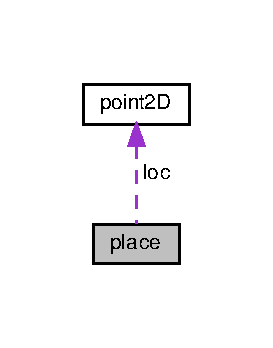
\includegraphics[width=131pt]{classplace__coll__graph}
\end{center}
\end{figure}
\subsection*{Public Member Functions}
\begin{DoxyCompactItemize}
\item 
\mbox{\Hypertarget{classplace_ade1afd10cb254434214fb43d95dd6a4f}\label{classplace_ade1afd10cb254434214fb43d95dd6a4f}} 
{\bfseries place} (unsigned t)
\item 
\mbox{\Hypertarget{classplace_a88cfb493e57ceabe0753ab98b2e6dac5}\label{classplace_a88cfb493e57ceabe0753ab98b2e6dac5}} 
void {\bfseries init} ()
\item 
\mbox{\Hypertarget{classplace_a3b3fd9f79977012225fefffaf0e5f5d4}\label{classplace_a3b3fd9f79977012225fefffaf0e5f5d4}} 
void {\bfseries set\+Type} (unsigned t)
\item 
\mbox{\Hypertarget{classplace_a67e4c5da30e53886486fe8ec57467ed2}\label{classplace_a67e4c5da30e53886486fe8ec57467ed2}} 
void {\bfseries set\+Location} (\mbox{\hyperlink{classpoint2D}{point2D}} p)
\item 
\mbox{\Hypertarget{classplace_a2175356d103d8aedb4c355d7436f9d56}\label{classplace_a2175356d103d8aedb4c355d7436f9d56}} 
void {\bfseries set\+Location} (double x, double y)
\item 
\mbox{\Hypertarget{classplace_a41e21b063e8db8099c80f4fe13417b76}\label{classplace_a41e21b063e8db8099c80f4fe13417b76}} 
\mbox{\hyperlink{classpoint2D}{point2D}} {\bfseries get\+Location} ()
\item 
\mbox{\Hypertarget{classplace_acc6dddccc006b7587ac99d083f22ce4d}\label{classplace_acc6dddccc006b7587ac99d083f22ce4d}} 
void {\bfseries increment\+Work\+Force} ()
\item 
\mbox{\Hypertarget{classplace_a327ed403446309536953b7cf9ba51fe2}\label{classplace_a327ed403446309536953b7cf9ba51fe2}} 
unsigned {\bfseries place\+Type} ()
\item 
\mbox{\Hypertarget{classplace_af0d1fb750a7f800a4ae8245932a1709c}\label{classplace_af0d1fb750a7f800a4ae8245932a1709c}} 
unsigned {\bfseries ID} ()
\item 
\mbox{\Hypertarget{classplace_ab63a396b9781a5f7d69a9f7b5ce32a1e}\label{classplace_ab63a396b9781a5f7d69a9f7b5ce32a1e}} 
double {\bfseries X} ()
\item 
\mbox{\Hypertarget{classplace_a4104729bc9904da36159775a7cf5ce1e}\label{classplace_a4104729bc9904da36159775a7cf5ce1e}} 
double {\bfseries Y} ()
\item 
\mbox{\Hypertarget{classplace_a06933a289fc55df54c622725e4227003}\label{classplace_a06933a289fc55df54c622725e4227003}} 
unsigned {\bfseries work\+Force\+Size} ()
\end{DoxyCompactItemize}
\subsection*{Public Attributes}
\begin{DoxyCompactItemize}
\item 
\mbox{\Hypertarget{classplace_a30abc26da34316006bac7d17398f0076}\label{classplace_a30abc26da34316006bac7d17398f0076}} 
\mbox{\hyperlink{classpoint2D}{point2D}} {\bfseries loc}
\end{DoxyCompactItemize}
\subsection*{Private Attributes}
\begin{DoxyCompactItemize}
\item 
\mbox{\Hypertarget{classplace_a905b649d1f98547cc33d49226f4e56e1}\label{classplace_a905b649d1f98547cc33d49226f4e56e1}} 
unsigned {\bfseries \+\_\+\+ID}
\item 
\mbox{\Hypertarget{classplace_a675f8c9a2bd0c57ac1aaf0364cd63411}\label{classplace_a675f8c9a2bd0c57ac1aaf0364cd63411}} 
unsigned {\bfseries \+\_\+work\+Force\+Size}
\item 
\mbox{\Hypertarget{classplace_ac74e8a9d1409cec4421a038885012a8b}\label{classplace_ac74e8a9d1409cec4421a038885012a8b}} 
unsigned {\bfseries \+\_\+capacity}
\item 
\mbox{\Hypertarget{classplace_a4289f32750fe9e9b0632afe207dd999b}\label{classplace_a4289f32750fe9e9b0632afe207dd999b}} 
unsigned {\bfseries \+\_\+type}
\end{DoxyCompactItemize}
\subsection*{Static Private Attributes}
\begin{DoxyCompactItemize}
\item 
\mbox{\Hypertarget{classplace_af35d12619e41bd59aa91db9977fc8dc9}\label{classplace_af35d12619e41bd59aa91db9977fc8dc9}} 
static unsigned {\bfseries idnum} =0
\end{DoxyCompactItemize}


\subsection{Detailed Description}
A place has x,y co-\/ordinates, and possibly a workforce and capacity. 

Definition at line 16 of file places.\+h.



The documentation for this class was generated from the following files\+:\begin{DoxyCompactItemize}
\item 
places.\+h\item 
places.\+cpp\end{DoxyCompactItemize}

\hypertarget{classplaces}{}\section{places Class Reference}
\label{classplaces}\index{places@{places}}


Places stores the place type index and a list of instantiated places.  




{\ttfamily \#include $<$places.\+h$>$}



Collaboration diagram for places\+:\nopagebreak
\begin{figure}[H]
\begin{center}
\leavevmode
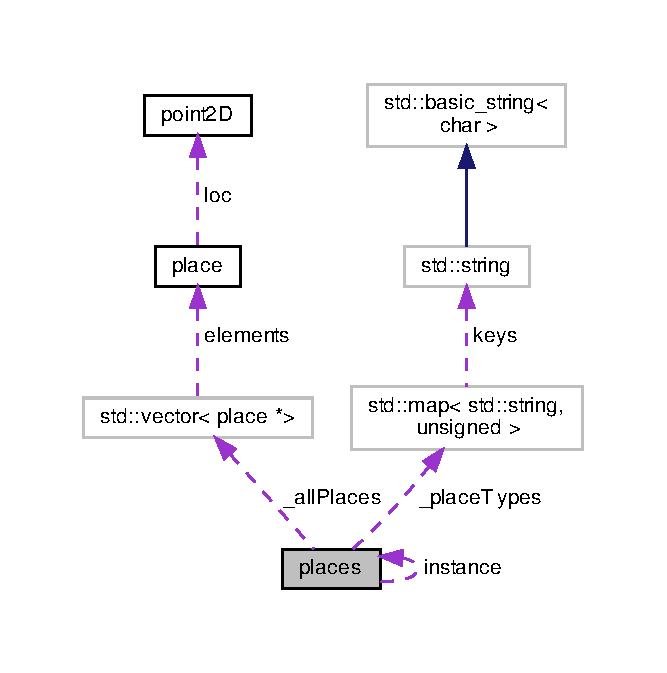
\includegraphics[width=320pt]{classplaces__coll__graph}
\end{center}
\end{figure}
\subsection*{Public Member Functions}
\begin{DoxyCompactItemize}
\item 
unsigned \mbox{\hyperlink{classplaces_a18b24350e2ad05ef273df442b6d22593}{operator\mbox{[}$\,$\mbox{]}}} (std\+::string)
\begin{DoxyCompactList}\small\item\em Return the type index index for a named place. \end{DoxyCompactList}\item 
void \mbox{\hyperlink{classplaces_ad126c2796c4fecad43f8e237ffde786d}{init}} ()
\begin{DoxyCompactList}\small\item\em Set up the index of place types and read in actual places. \end{DoxyCompactList}\item 
bool \mbox{\hyperlink{classplaces_a5ff3d2cd02c18f353ab15dd86f52e7be}{update}} ()
\begin{DoxyCompactList}\small\item\em Stub provided in case at some point the data in places becomes dynamic and needs its own updates. \end{DoxyCompactList}\item 
\mbox{\Hypertarget{classplaces_acd22734e55333fc53f937251f7f2ba4f}\label{classplaces_acd22734e55333fc53f937251f7f2ba4f}} 
void \mbox{\hyperlink{classplaces_acd22734e55333fc53f937251f7f2ba4f}{print\+Work\+Force\+Sizes}} ()
\begin{DoxyCompactList}\small\item\em Function to report how many people are currently working in the list of all places. \end{DoxyCompactList}\end{DoxyCompactItemize}
\subsection*{Static Public Member Functions}
\begin{DoxyCompactItemize}
\item 
static \mbox{\hyperlink{classplaces}{places}} \& \mbox{\hyperlink{classplaces_acb5dbcd8606a8a1ffbebc9fb5a3c8a5e}{get\+Instance}} ()
\begin{DoxyCompactList}\small\item\em Get a reference to the place class. \end{DoxyCompactList}\end{DoxyCompactItemize}
\subsection*{Static Public Attributes}
\begin{DoxyCompactItemize}
\item 
\mbox{\Hypertarget{classplaces_acac17c038967becf0ccaffbcc88e35fa}\label{classplaces_acac17c038967becf0ccaffbcc88e35fa}} 
static \mbox{\hyperlink{classplaces}{places}} $\ast$ \mbox{\hyperlink{classplaces_acac17c038967becf0ccaffbcc88e35fa}{instance}}
\begin{DoxyCompactList}\small\item\em The pointer that stores the instance of places. \end{DoxyCompactList}\item 
static unsigned \mbox{\hyperlink{classplaces_ab03feda32ddd4784c17de8b2185b3563}{unknown\+Type}} =std\+::numeric\+\_\+limits$<$unsigned$>$\+::max()
\begin{DoxyCompactList}\small\item\em Returned if there is no know place of this type. \end{DoxyCompactList}\end{DoxyCompactItemize}
\subsection*{Protected Member Functions}
\begin{DoxyCompactItemize}
\item 
\mbox{\hyperlink{classplaces_a1c4116c838392a6d35169126334f3f61}{places}} ()
\begin{DoxyCompactList}\small\item\em Private constructor can only be called by the class itself. \end{DoxyCompactList}\end{DoxyCompactItemize}
\subsection*{Protected Attributes}
\begin{DoxyCompactItemize}
\item 
std\+::vector$<$ \mbox{\hyperlink{classplace}{place}} $\ast$ $>$ \mbox{\hyperlink{classplaces_a2cb6b12513a2245fd06b567490229d89}{\+\_\+all\+Places}}
\begin{DoxyCompactList}\small\item\em A vector of pointers to all the places currently defined in the model. \end{DoxyCompactList}\item 
std\+::map$<$ std\+::string, unsigned $>$ \mbox{\hyperlink{classplaces_a7d5529185ae4635d2e2048b4ae475c12}{\+\_\+place\+Types}}
\begin{DoxyCompactList}\small\item\em The index of place types. \end{DoxyCompactList}\end{DoxyCompactItemize}


\subsection{Detailed Description}
Places stores the place type index and a list of instantiated places. 

There are two main data stuctures here\+: a vector of pointers to all the places, so that they can be iterated over or retrieved without reference to spatial position. Secondly there is an index that maps from strings to unsigned integers, so that places can be given an integer type. E.\+g. the string \char`\"{}hospital\char`\"{} might map to integer 0. These indices are set up in \mbox{\hyperlink{classplaces_ad126c2796c4fecad43f8e237ffde786d}{init()}} according to the order place types are listed in the csv file pointed at by parameters place\+Type\+File, This avoids having to store strings in other parts of the model\+: for example, the \mbox{\hyperlink{classsearchGrid}{search\+Grid}} stores places in each cell indexed by type. 

Definition at line 53 of file places.\+h.



\subsection{Constructor \& Destructor Documentation}
\mbox{\Hypertarget{classplaces_a1c4116c838392a6d35169126334f3f61}\label{classplaces_a1c4116c838392a6d35169126334f3f61}} 
\index{places@{places}!places@{places}}
\index{places@{places}!places@{places}}
\subsubsection{\texorpdfstring{places()}{places()}}
{\footnotesize\ttfamily places\+::places (\begin{DoxyParamCaption}{ }\end{DoxyParamCaption})\hspace{0.3cm}{\ttfamily [protected]}}



Private constructor can only be called by the class itself. 

Since this is singleton the contructor should only ever be called once. 

Definition at line 10 of file places.\+cpp.



\subsection{Member Function Documentation}
\mbox{\Hypertarget{classplaces_acb5dbcd8606a8a1ffbebc9fb5a3c8a5e}\label{classplaces_acb5dbcd8606a8a1ffbebc9fb5a3c8a5e}} 
\index{places@{places}!get\+Instance@{get\+Instance}}
\index{get\+Instance@{get\+Instance}!places@{places}}
\subsubsection{\texorpdfstring{get\+Instance()}{getInstance()}}
{\footnotesize\ttfamily \mbox{\hyperlink{classplaces}{places}} \& places\+::get\+Instance (\begin{DoxyParamCaption}{ }\end{DoxyParamCaption})\hspace{0.3cm}{\ttfamily [static]}}



Get a reference to the place class. 

\begin{DoxyReturn}{Returns}
places\& 
\end{DoxyReturn}


Definition at line 14 of file places.\+cpp.

\mbox{\Hypertarget{classplaces_ad126c2796c4fecad43f8e237ffde786d}\label{classplaces_ad126c2796c4fecad43f8e237ffde786d}} 
\index{places@{places}!init@{init}}
\index{init@{init}!places@{places}}
\subsubsection{\texorpdfstring{init()}{init()}}
{\footnotesize\ttfamily void places\+::init (\begin{DoxyParamCaption}{ }\end{DoxyParamCaption})}



Set up the index of place types and read in actual places. 

Caution with this function! Places are inserted into the \mbox{\hyperlink{classsearchGrid}{search\+Grid}} model\+::g so that they can be found by spatial searches. If at any point the grid is re-\/sized, then this data may become invalid. Important therefore to make sure this function is called {\itshape after} any grid re-\/sizing (which should in any case only happen during model initialisation) 

Definition at line 26 of file places.\+cpp.

\mbox{\Hypertarget{classplaces_a18b24350e2ad05ef273df442b6d22593}\label{classplaces_a18b24350e2ad05ef273df442b6d22593}} 
\index{places@{places}!operator\mbox{[}\mbox{]}@{operator[]}}
\index{operator\mbox{[}\mbox{]}@{operator[]}!places@{places}}
\subsubsection{\texorpdfstring{operator[]()}{operator[]()}}
{\footnotesize\ttfamily unsigned places\+::operator\mbox{[}$\,$\mbox{]} (\begin{DoxyParamCaption}\item[{std\+::string}]{s }\end{DoxyParamCaption})}



Return the type index index for a named place. 

If a string is given as an argument, and there is no corresponding key then \mbox{\hyperlink{classplaces_ab03feda32ddd4784c17de8b2185b3563}{places\+::unknown\+Type}} is returned


\begin{DoxyParams}{Parameters}
{\em s} & A string giving the name of the type of place \\
\hline
\end{DoxyParams}
\begin{DoxyReturn}{Returns}
unsigned int 
\end{DoxyReturn}


Definition at line 21 of file places.\+cpp.

\mbox{\Hypertarget{classplaces_a5ff3d2cd02c18f353ab15dd86f52e7be}\label{classplaces_a5ff3d2cd02c18f353ab15dd86f52e7be}} 
\index{places@{places}!update@{update}}
\index{update@{update}!places@{places}}
\subsubsection{\texorpdfstring{update()}{update()}}
{\footnotesize\ttfamily bool places\+::update (\begin{DoxyParamCaption}{ }\end{DoxyParamCaption})}



Stub provided in case at some point the data in places becomes dynamic and needs its own updates. 

\begin{DoxyReturn}{Returns}
bool 
\end{DoxyReturn}


Definition at line 47 of file places.\+cpp.



\subsection{Member Data Documentation}
\mbox{\Hypertarget{classplaces_a2cb6b12513a2245fd06b567490229d89}\label{classplaces_a2cb6b12513a2245fd06b567490229d89}} 
\index{places@{places}!\+\_\+all\+Places@{\+\_\+all\+Places}}
\index{\+\_\+all\+Places@{\+\_\+all\+Places}!places@{places}}
\subsubsection{\texorpdfstring{\+\_\+all\+Places}{\_allPlaces}}
{\footnotesize\ttfamily std\+::vector$<$\mbox{\hyperlink{classplace}{place}}$\ast$$>$ places\+::\+\_\+all\+Places\hspace{0.3cm}{\ttfamily [protected]}}



A vector of pointers to all the places currently defined in the model. 

Places is a singleton (there can only be one instance of this class in the model) 

Definition at line 68 of file places.\+h.

\mbox{\Hypertarget{classplaces_a7d5529185ae4635d2e2048b4ae475c12}\label{classplaces_a7d5529185ae4635d2e2048b4ae475c12}} 
\index{places@{places}!\+\_\+place\+Types@{\+\_\+place\+Types}}
\index{\+\_\+place\+Types@{\+\_\+place\+Types}!places@{places}}
\subsubsection{\texorpdfstring{\+\_\+place\+Types}{\_placeTypes}}
{\footnotesize\ttfamily std\+::map$<$std\+::string,unsigned$>$ places\+::\+\_\+place\+Types\hspace{0.3cm}{\ttfamily [protected]}}



The index of place types. 

Given a string as a key, this variable stores an index that can be used to refer to this type of place 

Definition at line 75 of file places.\+h.

\mbox{\Hypertarget{classplaces_ab03feda32ddd4784c17de8b2185b3563}\label{classplaces_ab03feda32ddd4784c17de8b2185b3563}} 
\index{places@{places}!unknown\+Type@{unknown\+Type}}
\index{unknown\+Type@{unknown\+Type}!places@{places}}
\subsubsection{\texorpdfstring{unknown\+Type}{unknownType}}
{\footnotesize\ttfamily unsigned places\+::unknown\+Type =std\+::numeric\+\_\+limits$<$unsigned$>$\+::max()\hspace{0.3cm}{\ttfamily [static]}}



Returned if there is no know place of this type. 

Currently set to the maxium value for an unsigned integer (unlikely ever to be this manby place types!) 

Definition at line 118 of file places.\+h.



The documentation for this class was generated from the following files\+:\begin{DoxyCompactItemize}
\item 
places.\+h\item 
places.\+cpp\end{DoxyCompactItemize}

\hypertarget{classpoint}{}\section{point Class Reference}
\label{classpoint}\index{point@{point}}


Inheritance diagram for point\+:\nopagebreak
\begin{figure}[H]
\begin{center}
\leavevmode
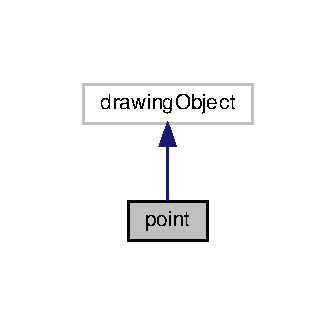
\includegraphics[width=161pt]{classpoint__inherit__graph}
\end{center}
\end{figure}


Collaboration diagram for point\+:\nopagebreak
\begin{figure}[H]
\begin{center}
\leavevmode
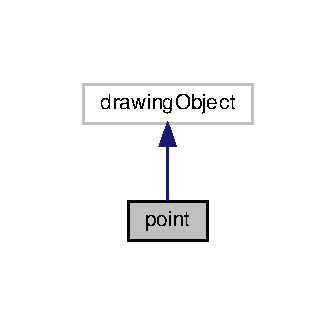
\includegraphics[width=161pt]{classpoint__coll__graph}
\end{center}
\end{figure}
\subsection*{Public Member Functions}
\begin{DoxyCompactItemize}
\item 
\mbox{\Hypertarget{classpoint_a5e1930bd8f6ebae2e840c1836b2e2875}\label{classpoint_a5e1930bd8f6ebae2e840c1836b2e2875}} 
{\bfseries point} (G\+Lfloat r=1, G\+Lfloat px=0., G\+Lfloat py=0., G\+Lfloat pz=0., G\+Luint rsx=15, G\+Luint rsy=15)
\item 
\mbox{\Hypertarget{classpoint_adb291571b18314e925e810f3a4340520}\label{classpoint_adb291571b18314e925e810f3a4340520}} 
void {\bfseries shape} ()
\end{DoxyCompactItemize}


\subsection{Detailed Description}


Definition at line 4 of file point.\+h.



The documentation for this class was generated from the following file\+:\begin{DoxyCompactItemize}
\item 
point.\+h\end{DoxyCompactItemize}

\hypertarget{classpoint2D}{}\section{point2D Class Reference}
\label{classpoint2D}\index{point2D@{point2D}}
\subsection*{Public Member Functions}
\begin{DoxyCompactItemize}
\item 
\mbox{\Hypertarget{classpoint2D_ad3c713839ca9768e41c295b2e6e5afa7}\label{classpoint2D_ad3c713839ca9768e41c295b2e6e5afa7}} 
{\bfseries point2D} (double x\+\_\+, double y\+\_\+)
\item 
\mbox{\Hypertarget{classpoint2D_ab5af14144bffe77818139d21003b58bb}\label{classpoint2D_ab5af14144bffe77818139d21003b58bb}} 
{\bfseries point2D} (const \mbox{\hyperlink{classpoint2D}{point2D}} \&p)
\item 
\mbox{\Hypertarget{classpoint2D_a34b676d196277da05f03e87dc2f88288}\label{classpoint2D_a34b676d196277da05f03e87dc2f88288}} 
bool {\bfseries operator==} (const \mbox{\hyperlink{classpoint2D}{point2D}} \&p)
\item 
\mbox{\Hypertarget{classpoint2D_a76074a1176a4618c53d3f043bfdf6c63}\label{classpoint2D_a76074a1176a4618c53d3f043bfdf6c63}} 
\mbox{\hyperlink{classpoint2D}{point2D}} {\bfseries operator+} (const \mbox{\hyperlink{classpoint2D}{point2D}} \&p)
\item 
\mbox{\Hypertarget{classpoint2D_a09800bd3d11ba62ff77016c8d120dad6}\label{classpoint2D_a09800bd3d11ba62ff77016c8d120dad6}} 
\mbox{\hyperlink{classpoint2D}{point2D}} {\bfseries operator-\/} (const \mbox{\hyperlink{classpoint2D}{point2D}} \&p)
\item 
\mbox{\Hypertarget{classpoint2D_ae82aa8f1fb54ea829b5d96bf0abe2ee4}\label{classpoint2D_ae82aa8f1fb54ea829b5d96bf0abe2ee4}} 
\mbox{\hyperlink{classpoint2D}{point2D}} {\bfseries operator-\/} (const double \&p)
\item 
\mbox{\Hypertarget{classpoint2D_aa083eccf18a944e03f097ec386d90f41}\label{classpoint2D_aa083eccf18a944e03f097ec386d90f41}} 
\mbox{\hyperlink{classpoint2D}{point2D}} {\bfseries operator/} (const double \&d)
\item 
\mbox{\Hypertarget{classpoint2D_a99f2c435a66f29b578cfbe038e3b0a4f}\label{classpoint2D_a99f2c435a66f29b578cfbe038e3b0a4f}} 
\mbox{\hyperlink{classpoint2D}{point2D}} {\bfseries operator$\ast$} (const double \&d)
\item 
\mbox{\Hypertarget{classpoint2D_ae51e5cac280000178e5e1f195a0d261e}\label{classpoint2D_ae51e5cac280000178e5e1f195a0d261e}} 
double {\bfseries size} ()
\end{DoxyCompactItemize}
\subsection*{Public Attributes}
\begin{DoxyCompactItemize}
\item 
\mbox{\Hypertarget{classpoint2D_ade69032d2a9596dfd5c2b3ee29551569}\label{classpoint2D_ade69032d2a9596dfd5c2b3ee29551569}} 
double {\bfseries x}
\item 
\mbox{\Hypertarget{classpoint2D_aeb2d0d7a7919611c9b6022fec6ca0bc6}\label{classpoint2D_aeb2d0d7a7919611c9b6022fec6ca0bc6}} 
double {\bfseries y}
\item 
\mbox{\Hypertarget{classpoint2D_ac6fadd42bce37bf8d54665b350246768}\label{classpoint2D_ac6fadd42bce37bf8d54665b350246768}} 
int {\bfseries cell\+Index}
\end{DoxyCompactItemize}


\subsection{Detailed Description}


Definition at line 4 of file point2\+D.\+h.



The documentation for this class was generated from the following file\+:\begin{DoxyCompactItemize}
\item 
point2\+D.\+h\end{DoxyCompactItemize}

\hypertarget{classpopulationBuilder}{}\section{population\+Builder Class Reference}
\label{classpopulationBuilder}\index{population\+Builder@{population\+Builder}}


Collaboration diagram for population\+Builder\+:
\nopagebreak
\begin{figure}[H]
\begin{center}
\leavevmode
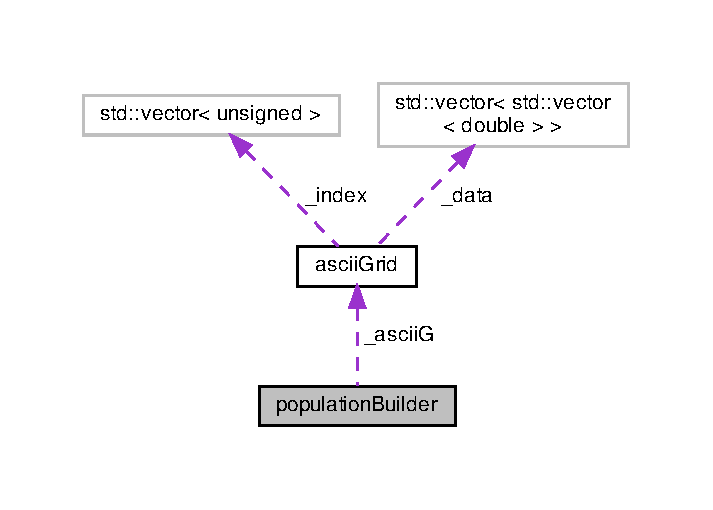
\includegraphics[width=342pt]{classpopulationBuilder__coll__graph}
\end{center}
\end{figure}
\subsection*{Public Member Functions}
\begin{DoxyCompactItemize}
\item 
\mbox{\Hypertarget{classpopulationBuilder_a464b444e7d17fcdcce70753eb71791d1}\label{classpopulationBuilder_a464b444e7d17fcdcce70753eb71791d1}} 
\mbox{\hyperlink{classpoint2D}{point2D}} {\bfseries get\+Next\+Location} ()
\item 
\mbox{\Hypertarget{classpopulationBuilder_aefaffd4d8bdadd7f1ff58e604095a9b0}\label{classpopulationBuilder_aefaffd4d8bdadd7f1ff58e604095a9b0}} 
void {\bfseries start\+Count} ()
\item 
\mbox{\Hypertarget{classpopulationBuilder_a5a288f060298983de16fc85972614a3a}\label{classpopulationBuilder_a5a288f060298983de16fc85972614a3a}} 
int {\bfseries person\+At\+Next\+Location} ()
\item 
\mbox{\Hypertarget{classpopulationBuilder_a64f8562892260879b013d8b07cd2727e}\label{classpopulationBuilder_a64f8562892260879b013d8b07cd2727e}} 
void {\bfseries configure\+Population} (std\+::vector$<$ \mbox{\hyperlink{classagent}{agent}} $\ast$$>$ \&\mbox{\hyperlink{classagents}{agents}})
\end{DoxyCompactItemize}
\subsection*{Private Member Functions}
\begin{DoxyCompactItemize}
\item 
\mbox{\Hypertarget{classpopulationBuilder_a275a5768bd4eebcb6188a46c4f0938d3}\label{classpopulationBuilder_a275a5768bd4eebcb6188a46c4f0938d3}} 
void {\bfseries retired} (\mbox{\hyperlink{classagent}{agent}} $\ast$)
\item 
\mbox{\Hypertarget{classpopulationBuilder_a18fbed9af426b8063f58e60159a2d5e8}\label{classpopulationBuilder_a18fbed9af426b8063f58e60159a2d5e8}} 
void {\bfseries worker} (\mbox{\hyperlink{classagent}{agent}} $\ast$)
\item 
\mbox{\Hypertarget{classpopulationBuilder_a3f2a99cff69c7003c5770ba970cfff71}\label{classpopulationBuilder_a3f2a99cff69c7003c5770ba970cfff71}} 
void {\bfseries university} (\mbox{\hyperlink{classagent}{agent}} $\ast$)
\item 
\mbox{\Hypertarget{classpopulationBuilder_a0c30bc831b9eaeba7b2b58b950195eca}\label{classpopulationBuilder_a0c30bc831b9eaeba7b2b58b950195eca}} 
void {\bfseries sixthform} (\mbox{\hyperlink{classagent}{agent}} $\ast$)
\item 
\mbox{\Hypertarget{classpopulationBuilder_aa83d25930398df932ea6064ca9f9222c}\label{classpopulationBuilder_aa83d25930398df932ea6064ca9f9222c}} 
void {\bfseries schoolchild} (\mbox{\hyperlink{classagent}{agent}} $\ast$)
\item 
\mbox{\Hypertarget{classpopulationBuilder_a520ae0408fc41a6c495db1f12a365410}\label{classpopulationBuilder_a520ae0408fc41a6c495db1f12a365410}} 
void {\bfseries preschool} (\mbox{\hyperlink{classagent}{agent}} $\ast$)
\item 
\mbox{\Hypertarget{classpopulationBuilder_a0f15496718bade91156656ad422c1655}\label{classpopulationBuilder_a0f15496718bade91156656ad422c1655}} 
void {\bfseries set\+Sex} (\mbox{\hyperlink{classagent}{agent}} $\ast$a)
\item 
\mbox{\Hypertarget{classpopulationBuilder_a0f1780441694d2ba8f2a36d511b9ecf8}\label{classpopulationBuilder_a0f1780441694d2ba8f2a36d511b9ecf8}} 
void {\bfseries set\+Age} (\mbox{\hyperlink{classagent}{agent}} $\ast$a)
\item 
\mbox{\Hypertarget{classpopulationBuilder_acbd753c13135d99eafb765e84766fc42}\label{classpopulationBuilder_acbd753c13135d99eafb765e84766fc42}} 
void {\bfseries find\+Partner} (\mbox{\hyperlink{classagent}{agent}} $\ast$a)
\item 
\mbox{\Hypertarget{classpopulationBuilder_a7f881efce32f9db8130c2a249ef848e8}\label{classpopulationBuilder_a7f881efce32f9db8130c2a249ef848e8}} 
void {\bfseries find\+Parents} (\mbox{\hyperlink{classagent}{agent}} $\ast$a)
\item 
\mbox{\Hypertarget{classpopulationBuilder_a244b9e0257946a4232d81871ecd64510}\label{classpopulationBuilder_a244b9e0257946a4232d81871ecd64510}} 
void {\bfseries set\+Up\+Education} (\mbox{\hyperlink{classagent}{agent}} $\ast$a)
\item 
\mbox{\Hypertarget{classpopulationBuilder_ac4bfa711ab996539feed62d07e90a362}\label{classpopulationBuilder_ac4bfa711ab996539feed62d07e90a362}} 
void {\bfseries set\+Up\+Work} (std\+::vector$<$ \mbox{\hyperlink{classagent}{agent}} $\ast$$>$ \&)
\item 
\mbox{\Hypertarget{classpopulationBuilder_a3ed4eec75d5afea0f92f799422cbfab9}\label{classpopulationBuilder_a3ed4eec75d5afea0f92f799422cbfab9}} 
void {\bfseries find\+Friends} (\mbox{\hyperlink{classagent}{agent}} $\ast$a)
\item 
\mbox{\Hypertarget{classpopulationBuilder_ad3cfae964af09027db5332c60a3a4eb7}\label{classpopulationBuilder_ad3cfae964af09027db5332c60a3a4eb7}} 
double {\bfseries commute\+Distance} ()
\end{DoxyCompactItemize}
\subsection*{Private Attributes}
\begin{DoxyCompactItemize}
\item 
\mbox{\Hypertarget{classpopulationBuilder_a1fe4d46bd4dfdb4dc4a3f5d79b0da405}\label{classpopulationBuilder_a1fe4d46bd4dfdb4dc4a3f5d79b0da405}} 
unsigned {\bfseries \+\_\+iter}
\item 
\mbox{\Hypertarget{classpopulationBuilder_a90fb547f1060562da92d12ab3b766d44}\label{classpopulationBuilder_a90fb547f1060562da92d12ab3b766d44}} 
double {\bfseries \+\_\+remaining\+Here}
\item 
\mbox{\Hypertarget{classpopulationBuilder_a1e7ee4d3dc120ae768187b223c20352e}\label{classpopulationBuilder_a1e7ee4d3dc120ae768187b223c20352e}} 
double {\bfseries \+\_\+frac}
\item 
\mbox{\Hypertarget{classpopulationBuilder_abd9d67fdeb86c61aa7ed60dd41095e19}\label{classpopulationBuilder_abd9d67fdeb86c61aa7ed60dd41095e19}} 
\mbox{\hyperlink{classasciiGrid}{ascii\+Grid}} {\bfseries \+\_\+asciiG}
\item 
\mbox{\Hypertarget{classpopulationBuilder_a626bdcad8632e6125fbb96b5c4c19fe1}\label{classpopulationBuilder_a626bdcad8632e6125fbb96b5c4c19fe1}} 
unsigned {\bfseries \+\_\+working\+Pop}
\end{DoxyCompactItemize}


\subsection{Detailed Description}


Definition at line 10 of file population\+Builder.\+h.



The documentation for this class was generated from the following files\+:\begin{DoxyCompactItemize}
\item 
population\+Builder.\+h\item 
population\+Builder.\+cpp\end{DoxyCompactItemize}

\hypertarget{classprocess}{}\section{process Class Reference}
\label{classprocess}\index{process@{process}}


Inheritance diagram for process\+:
\nopagebreak
\begin{figure}[H]
\begin{center}
\leavevmode
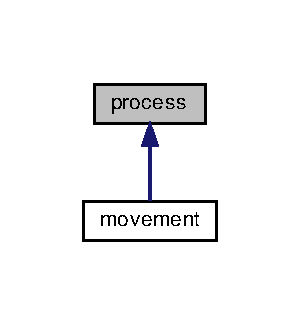
\includegraphics[width=144pt]{classprocess__inherit__graph}
\end{center}
\end{figure}


Collaboration diagram for process\+:
\nopagebreak
\begin{figure}[H]
\begin{center}
\leavevmode
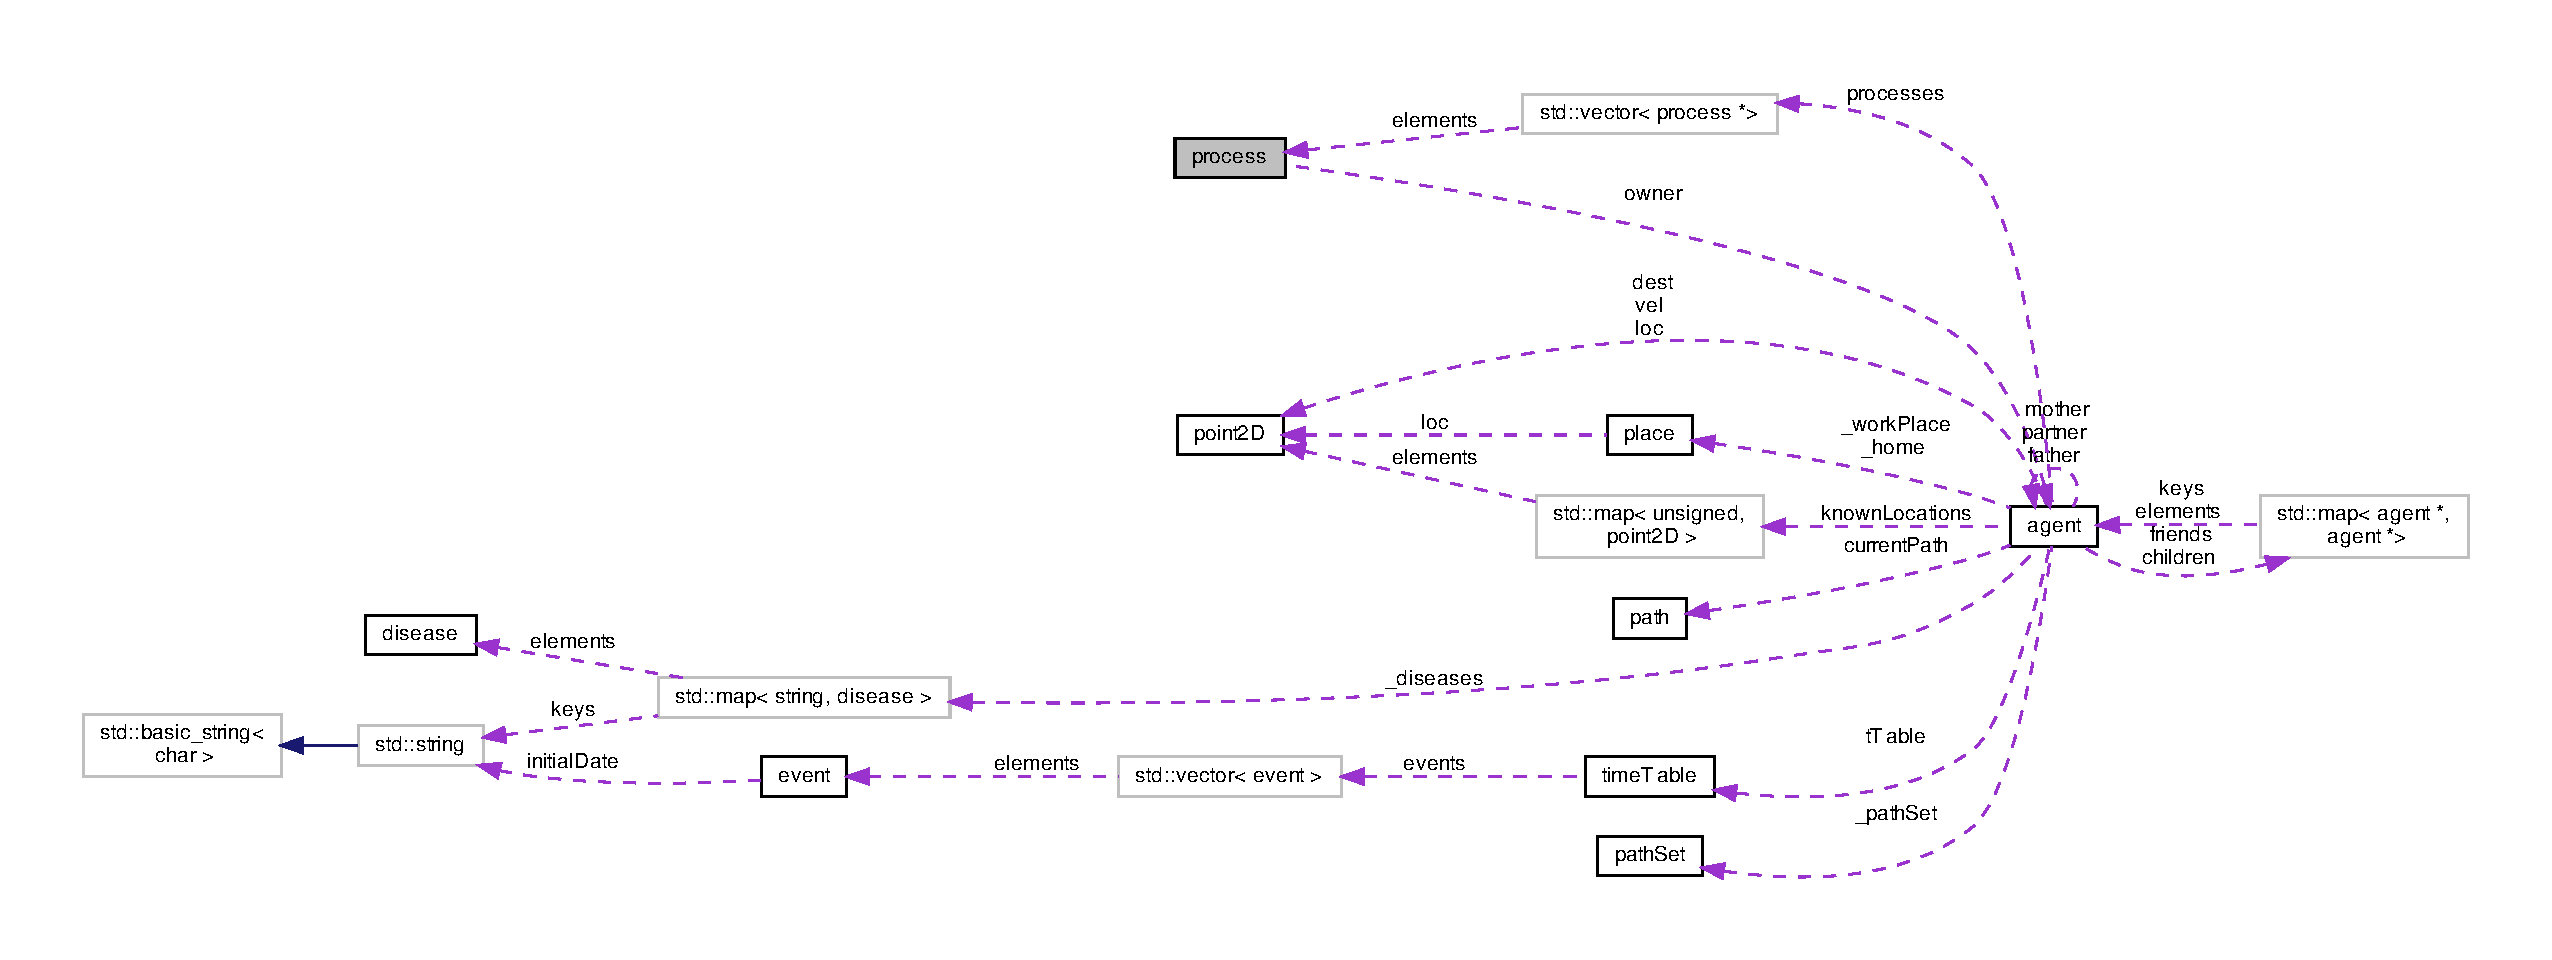
\includegraphics[width=350pt]{classprocess__coll__graph}
\end{center}
\end{figure}
\subsection*{Public Member Functions}
\begin{DoxyCompactItemize}
\item 
\mbox{\Hypertarget{classprocess_ab165eda9f0877f7c9b51b7e8a20090cb}\label{classprocess_ab165eda9f0877f7c9b51b7e8a20090cb}} 
{\bfseries process} (\mbox{\hyperlink{classagent}{agent}} $\ast$o)
\item 
\mbox{\Hypertarget{classprocess_a01cbd2a12c5ebb9f0d26ab0af1af1698}\label{classprocess_a01cbd2a12c5ebb9f0d26ab0af1af1698}} 
virtual void {\bfseries pre\+Update} ()
\item 
\mbox{\Hypertarget{classprocess_a221e8cbecf1f1b241e649db12cbea25f}\label{classprocess_a221e8cbecf1f1b241e649db12cbea25f}} 
virtual void {\bfseries update} ()
\item 
\mbox{\Hypertarget{classprocess_a3c856111d8e7c3e123ffb826ed1c4cd1}\label{classprocess_a3c856111d8e7c3e123ffb826ed1c4cd1}} 
virtual void {\bfseries apply\+Update} ()
\end{DoxyCompactItemize}
\subsection*{Public Attributes}
\begin{DoxyCompactItemize}
\item 
\mbox{\Hypertarget{classprocess_a6f930d4d4d03ac802ac349ef7373a9c5}\label{classprocess_a6f930d4d4d03ac802ac349ef7373a9c5}} 
\mbox{\hyperlink{classagent}{agent}} $\ast$ {\bfseries owner}
\end{DoxyCompactItemize}


\subsection{Detailed Description}


Definition at line 6 of file process.\+h.



The documentation for this class was generated from the following file\+:\begin{DoxyCompactItemize}
\item 
process.\+h\end{DoxyCompactItemize}

\hypertarget{classrandomizer}{}\section{randomizer Class Reference}
\label{classrandomizer}\index{randomizer@{randomizer}}
\subsection*{Public Member Functions}
\begin{DoxyCompactItemize}
\item 
\mbox{\Hypertarget{classrandomizer_ae175fffeb1c48d064973e33b3e11b9a0}\label{classrandomizer_ae175fffeb1c48d064973e33b3e11b9a0}} 
double {\bfseries number} ()
\item 
\mbox{\Hypertarget{classrandomizer_ad360ae291abce71d660ca8cadb344b00}\label{classrandomizer_ad360ae291abce71d660ca8cadb344b00}} 
void {\bfseries set\+Seed} (int s)
\end{DoxyCompactItemize}
\subsection*{Private Attributes}
\begin{DoxyCompactItemize}
\item 
\mbox{\Hypertarget{classrandomizer_a538d8fc8e95d8c64654d6b3354745194}\label{classrandomizer_a538d8fc8e95d8c64654d6b3354745194}} 
std\+::uniform\+\_\+real\+\_\+distribution {\bfseries uniform\+\_\+dist}
\item 
\mbox{\Hypertarget{classrandomizer_a8c1820ea3c64a67bf48fca01cb68a310}\label{classrandomizer_a8c1820ea3c64a67bf48fca01cb68a310}} 
std\+::mt19937 {\bfseries twister}
\end{DoxyCompactItemize}


\subsection{Detailed Description}


Definition at line 19 of file model.\+h.



The documentation for this class was generated from the following file\+:\begin{DoxyCompactItemize}
\item 
\mbox{\hyperlink{model_8h}{model.\+h}}\end{DoxyCompactItemize}

\hypertarget{classreadcsv}{}\section{readcsv Class Reference}
\label{classreadcsv}\index{readcsv@{readcsv}}


Collaboration diagram for readcsv\+:\nopagebreak
\begin{figure}[H]
\begin{center}
\leavevmode
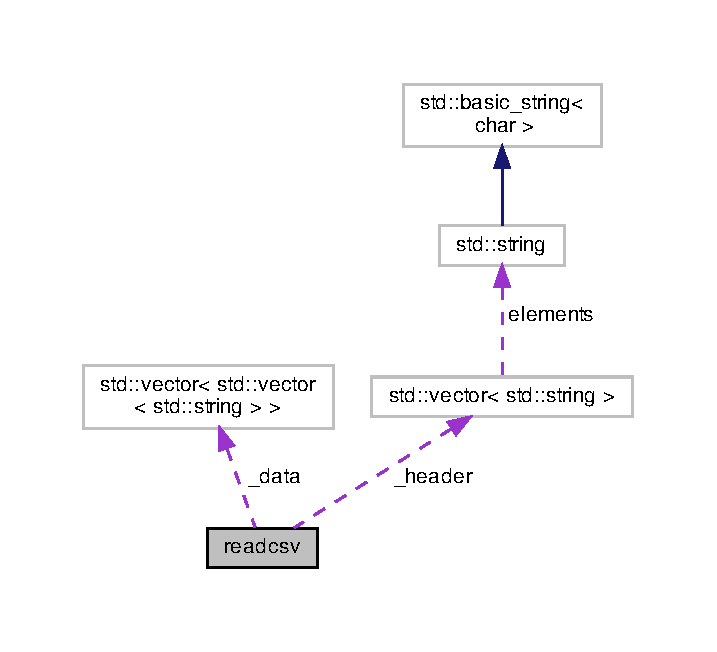
\includegraphics[width=344pt]{classreadcsv__coll__graph}
\end{center}
\end{figure}
\subsection*{Public Member Functions}
\begin{DoxyCompactItemize}
\item 
\mbox{\Hypertarget{classreadcsv_aa54ddf1101a8f8ab341fefd53bcfa800}\label{classreadcsv_aa54ddf1101a8f8ab341fefd53bcfa800}} 
{\bfseries readcsv} (std\+::string, bool header=true, bool commented=true)
\item 
\mbox{\Hypertarget{classreadcsv_a1334e39bd41afbdd8a1d494d23c65a43}\label{classreadcsv_a1334e39bd41afbdd8a1d494d23c65a43}} 
std\+::vector$<$ std\+::string $>$ {\bfseries operator\mbox{[}$\,$\mbox{]}} (unsigned i)
\item 
\mbox{\Hypertarget{classreadcsv_a6ed1061ac00e32b2db88df7ffc8ce3ed}\label{classreadcsv_a6ed1061ac00e32b2db88df7ffc8ce3ed}} 
void {\bfseries read\+File} (const std\+::string \&, bool)
\item 
\mbox{\Hypertarget{classreadcsv_a9296a02467fd317c09b72280cb34aff5}\label{classreadcsv_a9296a02467fd317c09b72280cb34aff5}} 
void {\bfseries read\+Data} (std\+::ifstream \&)
\item 
\mbox{\Hypertarget{classreadcsv_a790283b0e5a8c927c6fc21c99bfc7db3}\label{classreadcsv_a790283b0e5a8c927c6fc21c99bfc7db3}} 
void {\bfseries read\+Header} (std\+::ifstream \&)
\item 
\mbox{\Hypertarget{classreadcsv_a738276a30d4f0f01e70a62765ebab3c2}\label{classreadcsv_a738276a30d4f0f01e70a62765ebab3c2}} 
std\+::vector$<$ std\+::string $>$ \& {\bfseries get\+Header} ()
\item 
\mbox{\Hypertarget{classreadcsv_af5a63a92698cf6a511d90e8fe66c1d85}\label{classreadcsv_af5a63a92698cf6a511d90e8fe66c1d85}} 
unsigned {\bfseries nrows} ()
\end{DoxyCompactItemize}
\subsection*{Private Member Functions}
\begin{DoxyCompactItemize}
\item 
\mbox{\Hypertarget{classreadcsv_a9d68415134bb866f2162a6f993d5aae2}\label{classreadcsv_a9d68415134bb866f2162a6f993d5aae2}} 
const std\+::vector$<$ std\+::string $>$ {\bfseries String\+To\+Words} (const std\+::string \&, const char) const
\item 
\mbox{\Hypertarget{classreadcsv_af74454e2364f534458e58767bd2074e3}\label{classreadcsv_af74454e2364f534458e58767bd2074e3}} 
const std\+::vector$<$ double $>$ {\bfseries Line\+To\+Double} (const std\+::string \&, const char) const
\item 
\mbox{\Hypertarget{classreadcsv_a7e904a604d14230497bd13c479ebffd8}\label{classreadcsv_a7e904a604d14230497bd13c479ebffd8}} 
double {\bfseries String\+To\+Double} (const std\+::string \&string) const
\item 
\mbox{\Hypertarget{classreadcsv_a2332d4c46f12bfb30cf4302019eccf24}\label{classreadcsv_a2332d4c46f12bfb30cf4302019eccf24}} 
int {\bfseries String\+To\+Int} (const std\+::string \&string) const
\end{DoxyCompactItemize}
\subsection*{Private Attributes}
\begin{DoxyCompactItemize}
\item 
\mbox{\Hypertarget{classreadcsv_a17c06fc645f0057e92fa3c0d55a58756}\label{classreadcsv_a17c06fc645f0057e92fa3c0d55a58756}} 
std\+::vector$<$ std\+::vector$<$ std\+::string $>$ $>$ {\bfseries \+\_\+data}
\item 
\mbox{\Hypertarget{classreadcsv_ab1eb6eeb66768505281335774feca2c1}\label{classreadcsv_ab1eb6eeb66768505281335774feca2c1}} 
std\+::vector$<$ std\+::string $>$ {\bfseries \+\_\+header}
\item 
\mbox{\Hypertarget{classreadcsv_ac2d3cd159870efc5c92ef977d32399f9}\label{classreadcsv_ac2d3cd159870efc5c92ef977d32399f9}} 
char {\bfseries \+\_\+comment\+Character}
\end{DoxyCompactItemize}


\subsection{Detailed Description}


Definition at line 12 of file readcsv.\+h.



The documentation for this class was generated from the following files\+:\begin{DoxyCompactItemize}
\item 
readcsv.\+h\item 
readcsv.\+cpp\end{DoxyCompactItemize}

\hypertarget{classsearchGrid}{}\section{search\+Grid Class Reference}
\label{classsearchGrid}\index{search\+Grid@{search\+Grid}}


Collaboration diagram for search\+Grid\+:\nopagebreak
\begin{figure}[H]
\begin{center}
\leavevmode
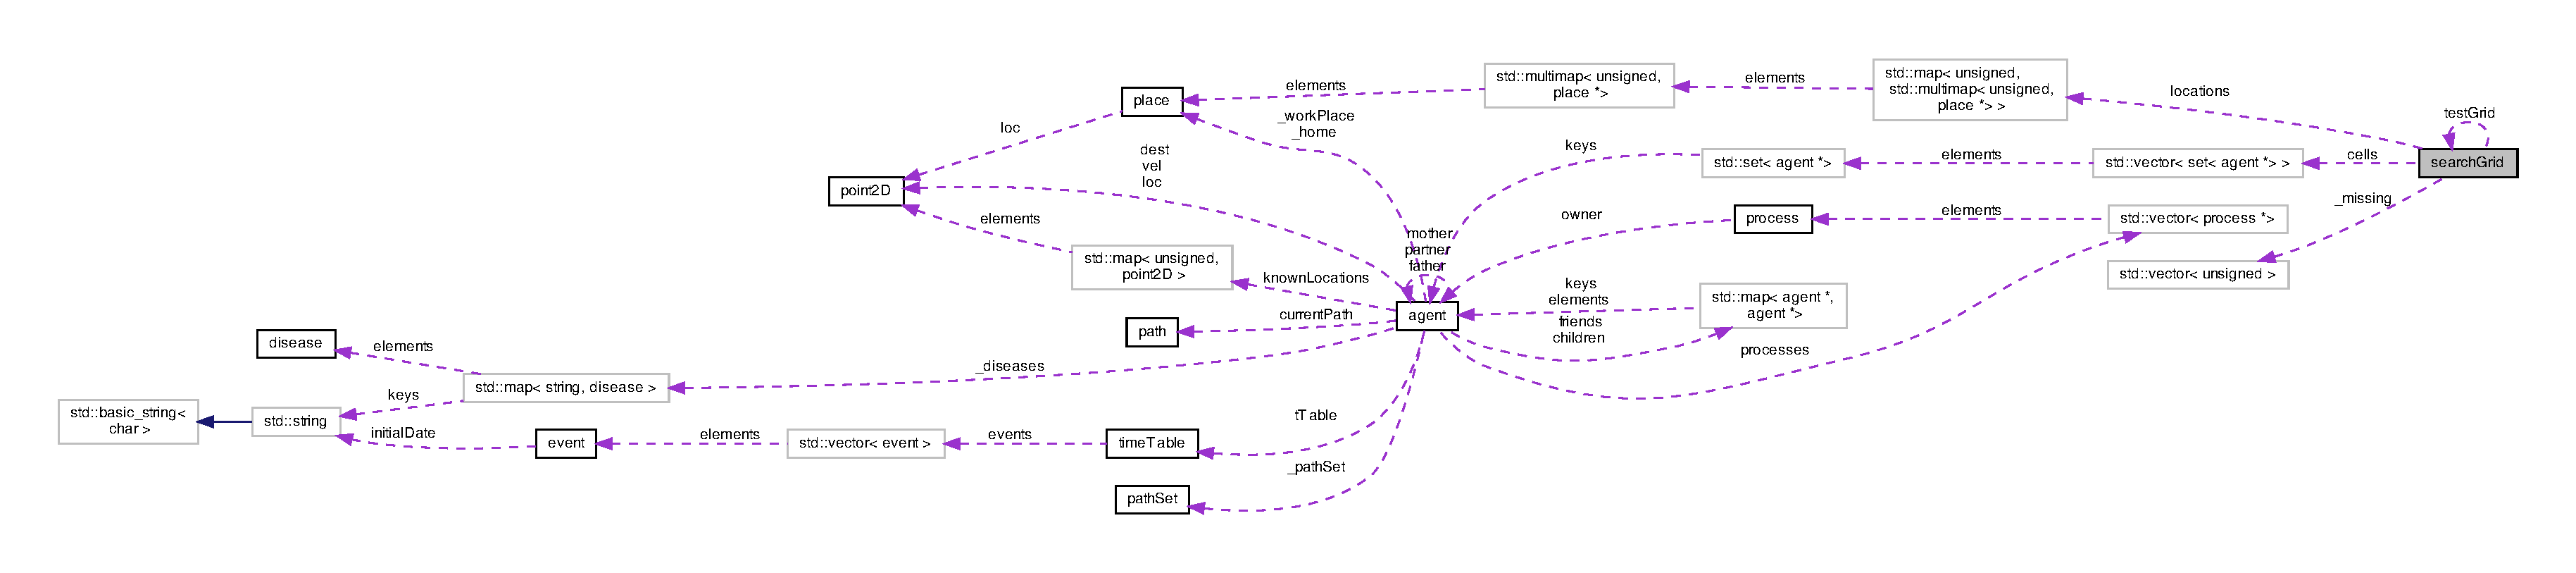
\includegraphics[width=350pt]{classsearchGrid__coll__graph}
\end{center}
\end{figure}
\subsection*{Public Member Functions}
\begin{DoxyCompactItemize}
\item 
\mbox{\Hypertarget{classsearchGrid_ae0a6729cbd7805277ffcb564b4a944ff}\label{classsearchGrid_ae0a6729cbd7805277ffcb564b4a944ff}} 
{\bfseries search\+Grid} (double, double, double, double, int, int)
\item 
\mbox{\Hypertarget{classsearchGrid_a884869df22304cc7de918b036b35e4cf}\label{classsearchGrid_a884869df22304cc7de918b036b35e4cf}} 
void {\bfseries init} (double, double, double, double, int, int)
\item 
\mbox{\Hypertarget{classsearchGrid_afe43b4b153b6eabbba15e9eb4cc4bcce}\label{classsearchGrid_afe43b4b153b6eabbba15e9eb4cc4bcce}} 
void {\bfseries init} ()
\item 
\mbox{\Hypertarget{classsearchGrid_a1dc5fd0533064d865f2ad0fcd4803f7c}\label{classsearchGrid_a1dc5fd0533064d865f2ad0fcd4803f7c}} 
void {\bfseries resize} (double, double, double, double, int, int)
\item 
\mbox{\Hypertarget{classsearchGrid_a25942068c892186e3000e219e28ef7f1}\label{classsearchGrid_a25942068c892186e3000e219e28ef7f1}} 
int {\bfseries find\+Cell\+Index} (double, double)
\item 
\mbox{\Hypertarget{classsearchGrid_accff7a0116d833e45b7b70e56768b2ab}\label{classsearchGrid_accff7a0116d833e45b7b70e56768b2ab}} 
void {\bfseries add} (\mbox{\hyperlink{classagent}{agent}} $\ast$)
\item 
\mbox{\Hypertarget{classsearchGrid_a866061b0de28991376b91c12b92300e5}\label{classsearchGrid_a866061b0de28991376b91c12b92300e5}} 
void {\bfseries remove} (\mbox{\hyperlink{classagent}{agent}} $\ast$)
\item 
\mbox{\Hypertarget{classsearchGrid_a58b0b4ced44c2a9585f2fe5d130c15d5}\label{classsearchGrid_a58b0b4ced44c2a9585f2fe5d130c15d5}} 
void {\bfseries add} (\mbox{\hyperlink{classplace}{place}} $\ast$)
\item 
\mbox{\Hypertarget{classsearchGrid_a183584d811404b032cd6eca009100bce}\label{classsearchGrid_a183584d811404b032cd6eca009100bce}} 
void {\bfseries remove} (\mbox{\hyperlink{classplace}{place}} $\ast$)
\item 
\mbox{\Hypertarget{classsearchGrid_a1658b9e34fe5af92cf5370fbd8283a85}\label{classsearchGrid_a1658b9e34fe5af92cf5370fbd8283a85}} 
vector$<$ \mbox{\hyperlink{classplace}{place}} $\ast$ $>$ {\bfseries in\+Radius} (\mbox{\hyperlink{classagent}{agent}} $\ast$, unsigned, double)
\item 
\mbox{\Hypertarget{classsearchGrid_a0b410acf9c8c7e1fb394538a978558f9}\label{classsearchGrid_a0b410acf9c8c7e1fb394538a978558f9}} 
void {\bfseries in\+Dist} (int, float, \mbox{\hyperlink{classagent}{agent}} $\ast$, unsigned, vector$<$ std\+::pair$<$ \mbox{\hyperlink{classplace}{place}} $\ast$, double $>$$>$ \&)
\item 
\mbox{\Hypertarget{classsearchGrid_a4b265b6f595070c5aa53e8c9be4cdcc3}\label{classsearchGrid_a4b265b6f595070c5aa53e8c9be4cdcc3}} 
void {\bfseries erase\+All} ()
\item 
\mbox{\Hypertarget{classsearchGrid_af88dcb0059b356e4589f07fc7789a829}\label{classsearchGrid_af88dcb0059b356e4589f07fc7789a829}} 
void {\bfseries check} ()
\item 
\mbox{\Hypertarget{classsearchGrid_ab1753e98c052effea4ff86976648a34e}\label{classsearchGrid_ab1753e98c052effea4ff86976648a34e}} 
void {\bfseries check} (\mbox{\hyperlink{classagent}{agent}} $\ast$)
\item 
\mbox{\Hypertarget{classsearchGrid_a60d9100d9505f9683d0e81a5a2394bef}\label{classsearchGrid_a60d9100d9505f9683d0e81a5a2394bef}} 
void {\bfseries check} (vector$<$ \mbox{\hyperlink{classagent}{agent}} $\ast$$>$ \&)
\item 
\mbox{\Hypertarget{classsearchGrid_a4318a1602cc5f146f8c181b827578888}\label{classsearchGrid_a4318a1602cc5f146f8c181b827578888}} 
void {\bfseries update} ()
\item 
\mbox{\Hypertarget{classsearchGrid_afec32e1fa615155a897d734c1bf7a27f}\label{classsearchGrid_afec32e1fa615155a897d734c1bf7a27f}} 
\mbox{\hyperlink{classpoint2D}{point2D}} {\bfseries get\+Random\+Point} ()
\item 
\mbox{\Hypertarget{classsearchGrid_a8695b1f2b62492cbe41083ac8d3758fb}\label{classsearchGrid_a8695b1f2b62492cbe41083ac8d3758fb}} 
vector$<$ \mbox{\hyperlink{classagent}{agent}} $\ast$ $>$ {\bfseries here} (\mbox{\hyperlink{classagent}{agent}} $\ast$)
\item 
\mbox{\Hypertarget{classsearchGrid_a99945ae6845a2e1074062e869c69c3e2}\label{classsearchGrid_a99945ae6845a2e1074062e869c69c3e2}} 
vector$<$ \mbox{\hyperlink{classagent}{agent}} $\ast$ $>$ {\bfseries in\+Radius} (\mbox{\hyperlink{classagent}{agent}} $\ast$, double)
\item 
\mbox{\Hypertarget{classsearchGrid_aad8ab42926dab85d6f4afc5084bc532c}\label{classsearchGrid_aad8ab42926dab85d6f4afc5084bc532c}} 
vector$<$ \mbox{\hyperlink{classagent}{agent}} $\ast$ $>$ {\bfseries in\+Square\+Region} (double, double, double)
\item 
\mbox{\Hypertarget{classsearchGrid_a7592f935d933f0554626e1fbb5afae35}\label{classsearchGrid_a7592f935d933f0554626e1fbb5afae35}} 
void {\bfseries in\+Square} (unsigned, double, double, double, double, vector$<$ \mbox{\hyperlink{classagent}{agent}} $\ast$$>$ \&)
\item 
\mbox{\Hypertarget{classsearchGrid_a8e57ece6343c3a2671670dd1e1f7656b}\label{classsearchGrid_a8e57ece6343c3a2671670dd1e1f7656b}} 
vector$<$ \mbox{\hyperlink{classagent}{agent}} $\ast$ $>$ {\bfseries neighbours4} (\mbox{\hyperlink{classagent}{agent}} $\ast$)
\item 
\mbox{\Hypertarget{classsearchGrid_ad87996d5112f98ed4be35527adffe48f}\label{classsearchGrid_ad87996d5112f98ed4be35527adffe48f}} 
vector$<$ \mbox{\hyperlink{classagent}{agent}} $\ast$ $>$ {\bfseries neighbours} (\mbox{\hyperlink{classagent}{agent}} $\ast$)
\item 
\mbox{\Hypertarget{classsearchGrid_ae7c79d583f544a9a3a25876c91ef8b0e}\label{classsearchGrid_ae7c79d583f544a9a3a25876c91ef8b0e}} 
void {\bfseries in\+Cell} (int, vector$<$ \mbox{\hyperlink{classagent}{agent}} $\ast$$>$ \&)
\item 
\mbox{\Hypertarget{classsearchGrid_adbeb6c7d74d58cb5a3b524e031ddd67a}\label{classsearchGrid_adbeb6c7d74d58cb5a3b524e031ddd67a}} 
void {\bfseries in\+Dist} (int, float, \mbox{\hyperlink{classagent}{agent}} $\ast$, vector$<$ \mbox{\hyperlink{classagent}{agent}} $\ast$$>$ \&)
\item 
\mbox{\Hypertarget{classsearchGrid_ae0230d99ebe10057f8d68d4ee493ad7c}\label{classsearchGrid_ae0230d99ebe10057f8d68d4ee493ad7c}} 
void {\bfseries wrap\+Defaults} ()
\item 
\mbox{\Hypertarget{classsearchGrid_aa52dec523a80080bc41896f95ee1cda7}\label{classsearchGrid_aa52dec523a80080bc41896f95ee1cda7}} 
void {\bfseries set\+Toroidal} ()
\item 
\mbox{\Hypertarget{classsearchGrid_add3e2c63256224cd8cb60e67146d6c9e}\label{classsearchGrid_add3e2c63256224cd8cb60e67146d6c9e}} 
void {\bfseries set\+WrapX} ()
\item 
\mbox{\Hypertarget{classsearchGrid_ab2f7ffa1bade8bef49b309fe9c712f7a}\label{classsearchGrid_ab2f7ffa1bade8bef49b309fe9c712f7a}} 
void {\bfseries set\+WrapY} ()
\item 
\mbox{\Hypertarget{classsearchGrid_a962c2bc9e5faa1de1f93f97f9bff73f2}\label{classsearchGrid_a962c2bc9e5faa1de1f93f97f9bff73f2}} 
void {\bfseries set\+Hard\+Edged} ()
\item 
\mbox{\Hypertarget{classsearchGrid_ad5844f3b10d406c6597a9fce210542fa}\label{classsearchGrid_ad5844f3b10d406c6597a9fce210542fa}} 
void {\bfseries set\+HardX} ()
\item 
\mbox{\Hypertarget{classsearchGrid_a574631ef7a30ee6e6014c6b244c0bedf}\label{classsearchGrid_a574631ef7a30ee6e6014c6b244c0bedf}} 
void {\bfseries set\+HardY} ()
\item 
\mbox{\Hypertarget{classsearchGrid_a6eeb1f5f0b71d3fd42b2e46e05ef6aee}\label{classsearchGrid_a6eeb1f5f0b71d3fd42b2e46e05ef6aee}} 
void {\bfseries set\+Sphere} ()
\item 
\mbox{\Hypertarget{classsearchGrid_a5fbfb6aebb21878babbea169ca349da6}\label{classsearchGrid_a5fbfb6aebb21878babbea169ca349da6}} 
vector$<$ vector$<$ double $>$ $>$ {\bfseries count} ()
\item 
\mbox{\Hypertarget{classsearchGrid_a72b400c83b39a057dda2b5674096426a}\label{classsearchGrid_a72b400c83b39a057dda2b5674096426a}} 
vector$<$ vector$<$ double $>$ $>$ {\bfseries count} (std\+::function$<$ bool(\mbox{\hyperlink{classagent}{agent}} \&)$>$)
\item 
\mbox{\Hypertarget{classsearchGrid_a4a30a4f8ad6869b2545cce4c4302da97}\label{classsearchGrid_a4a30a4f8ad6869b2545cce4c4302da97}} 
vector$<$ vector$<$ double $>$ $>$ {\bfseries count} (double)
\item 
\mbox{\Hypertarget{classsearchGrid_ad1017a47c18bbd7629de91fa95fe9b25}\label{classsearchGrid_ad1017a47c18bbd7629de91fa95fe9b25}} 
vector$<$ vector$<$ double $>$ $>$ {\bfseries count} (std\+::function$<$ bool(\mbox{\hyperlink{classagent}{agent}} \&)$>$, double)
\item 
\mbox{\Hypertarget{classsearchGrid_ac89f7b99e981208fca229f14b8adf158}\label{classsearchGrid_ac89f7b99e981208fca229f14b8adf158}} 
vector$<$ vector$<$ double $>$ $>$ {\bfseries count} (double, double, double, double, double)
\item 
\mbox{\Hypertarget{classsearchGrid_a6275b77b36feced1a3c9d0cc4e5c2a65}\label{classsearchGrid_a6275b77b36feced1a3c9d0cc4e5c2a65}} 
vector$<$ vector$<$ double $>$ $>$ {\bfseries count} (std\+::function$<$ bool(\mbox{\hyperlink{classagent}{agent}} \&)$>$, double, double, double, double, double)
\item 
\mbox{\Hypertarget{classsearchGrid_a168c428c3266f675c136f74de18eaf1d}\label{classsearchGrid_a168c428c3266f675c136f74de18eaf1d}} 
\mbox{\hyperlink{classasciiGridFileWriter}{ascii\+Grid\+File\+Writer}} $\ast$ {\bfseries get\+Ascii\+File\+Writer} (const std\+::string \&, const std\+::string \&, double missing=-\/9999)
\item 
\mbox{\Hypertarget{classsearchGrid_ab4656e09087dd116575ddf4398993b21}\label{classsearchGrid_ab4656e09087dd116575ddf4398993b21}} 
\mbox{\hyperlink{classasciiGridFileWriter}{ascii\+Grid\+File\+Writer}} $\ast$ {\bfseries get\+Ascii\+File\+Writer} (const std\+::string \&, const std\+::string \&, const double, double missing=-\/9999)
\item 
\mbox{\Hypertarget{classsearchGrid_a6fa9553dcdcdf8c7560e1d3f47b44029}\label{classsearchGrid_a6fa9553dcdcdf8c7560e1d3f47b44029}} 
\mbox{\hyperlink{classasciiGridFileWriter}{ascii\+Grid\+File\+Writer}} $\ast$ {\bfseries get\+Ascii\+File\+Writer} (const std\+::string \&, const std\+::string \&, double, double, double, double, double, double missing=-\/9999)
\item 
\mbox{\Hypertarget{classsearchGrid_a949147bca8cf28dacf337e699fae0cb2}\label{classsearchGrid_a949147bca8cf28dacf337e699fae0cb2}} 
double {\bfseries x\+Origin} ()
\item 
\mbox{\Hypertarget{classsearchGrid_a65ff7a575de3afc49a95a3cc77fb3599}\label{classsearchGrid_a65ff7a575de3afc49a95a3cc77fb3599}} 
double {\bfseries y\+Origin} ()
\item 
\mbox{\Hypertarget{classsearchGrid_ab8c31f776c01275a1ff0af09b763ee40}\label{classsearchGrid_ab8c31f776c01275a1ff0af09b763ee40}} 
double {\bfseries x\+Size} ()
\item 
\mbox{\Hypertarget{classsearchGrid_a5c9c7f02ef536ac97f7195091539fd9d}\label{classsearchGrid_a5c9c7f02ef536ac97f7195091539fd9d}} 
double {\bfseries y\+Size} ()
\end{DoxyCompactItemize}
\subsection*{Static Public Member Functions}
\begin{DoxyCompactItemize}
\item 
\mbox{\Hypertarget{classsearchGrid_ae2382291485f9cd84753ba2ed54ebaf1}\label{classsearchGrid_ae2382291485f9cd84753ba2ed54ebaf1}} 
static void {\bfseries test} ()
\end{DoxyCompactItemize}
\subsection*{Public Attributes}
\begin{DoxyCompactItemize}
\item 
\mbox{\Hypertarget{classsearchGrid_aa3e3842edf57c7952163ca0e0d2f2558}\label{classsearchGrid_aa3e3842edf57c7952163ca0e0d2f2558}} 
bool {\bfseries dirty}
\end{DoxyCompactItemize}
\subsection*{Private Member Functions}
\begin{DoxyCompactItemize}
\item 
\mbox{\Hypertarget{classsearchGrid_a16674ff1034191fca07034a321ab58ce}\label{classsearchGrid_a16674ff1034191fca07034a321ab58ce}} 
void {\bfseries test\+Message} (string, bool)
\item 
\mbox{\Hypertarget{classsearchGrid_a0bd630ee87181f0d9dcc19105cf1155c}\label{classsearchGrid_a0bd630ee87181f0d9dcc19105cf1155c}} 
void {\bfseries wrap\+Coordinates} (\mbox{\hyperlink{classagent}{agent}} $\ast$)
\item 
\mbox{\Hypertarget{classsearchGrid_a9a62217ee00a8eb3490f6e504ce4d797}\label{classsearchGrid_a9a62217ee00a8eb3490f6e504ce4d797}} 
void {\bfseries wrap\+Coordinates} (\mbox{\hyperlink{classplace}{place}} $\ast$)
\item 
\mbox{\Hypertarget{classsearchGrid_a0d93e1c5a49ed0bb06a6a2bfdd0882f9}\label{classsearchGrid_a0d93e1c5a49ed0bb06a6a2bfdd0882f9}} 
void {\bfseries torus} (double \&, double \&)
\item 
\mbox{\Hypertarget{classsearchGrid_ab6311643aef00a7c2324c7508e5fcbf4}\label{classsearchGrid_ab6311643aef00a7c2324c7508e5fcbf4}} 
void {\bfseries cylinderX} (double \&)
\item 
\mbox{\Hypertarget{classsearchGrid_a528af7734ebf54aa8a2378f6871c029a}\label{classsearchGrid_a528af7734ebf54aa8a2378f6871c029a}} 
void {\bfseries cylinderY} (double \&)
\item 
\mbox{\Hypertarget{classsearchGrid_a80caf18fc9f6d6a47d140c82a67e9154}\label{classsearchGrid_a80caf18fc9f6d6a47d140c82a67e9154}} 
void {\bfseries sphere} (double \&, double \&)
\item 
\mbox{\Hypertarget{classsearchGrid_a2707bb2fb7ca5b386f9f437b7a2a1956}\label{classsearchGrid_a2707bb2fb7ca5b386f9f437b7a2a1956}} 
void {\bfseries hard\+Edges} (double \&, double \&)
\item 
\mbox{\Hypertarget{classsearchGrid_ae890b7d65535b733415110256a643d87}\label{classsearchGrid_ae890b7d65535b733415110256a643d87}} 
void {\bfseries hardX} (double \&)
\item 
\mbox{\Hypertarget{classsearchGrid_a091a3f2ed69bceb26ab1d2b95b4bd222}\label{classsearchGrid_a091a3f2ed69bceb26ab1d2b95b4bd222}} 
void {\bfseries hardY} (double \&)
\end{DoxyCompactItemize}
\subsection*{Private Attributes}
\begin{DoxyCompactItemize}
\item 
\mbox{\Hypertarget{classsearchGrid_abcbade9dd5c49d7f21f8ca4d2d389bb7}\label{classsearchGrid_abcbade9dd5c49d7f21f8ca4d2d389bb7}} 
vector$<$ set$<$ \mbox{\hyperlink{classagent}{agent}} $\ast$ $>$ $>$ {\bfseries cells}
\item 
\mbox{\Hypertarget{classsearchGrid_ae0a1425af35ac4aa652ed1e28b73a140}\label{classsearchGrid_ae0a1425af35ac4aa652ed1e28b73a140}} 
double {\bfseries x0}
\item 
\mbox{\Hypertarget{classsearchGrid_a6bdbc7c04a45f23877e566b643ea4642}\label{classsearchGrid_a6bdbc7c04a45f23877e566b643ea4642}} 
double {\bfseries y0}
\item 
\mbox{\Hypertarget{classsearchGrid_ae1d710e6d2dd455b9b69f3c48c43c0bf}\label{classsearchGrid_ae1d710e6d2dd455b9b69f3c48c43c0bf}} 
double {\bfseries \+\_\+x\+Size}
\item 
\mbox{\Hypertarget{classsearchGrid_ac49fab1f8a1706d1e65619ca2d587474}\label{classsearchGrid_ac49fab1f8a1706d1e65619ca2d587474}} 
double {\bfseries \+\_\+y\+Size}
\item 
\mbox{\Hypertarget{classsearchGrid_a66b87cd34dcd0a114c1295ac33304f08}\label{classsearchGrid_a66b87cd34dcd0a114c1295ac33304f08}} 
int {\bfseries Nx\+Cells}
\item 
\mbox{\Hypertarget{classsearchGrid_ae3b6fdc38063bf0609e49342af476c63}\label{classsearchGrid_ae3b6fdc38063bf0609e49342af476c63}} 
int {\bfseries Ny\+Cells}
\item 
\mbox{\Hypertarget{classsearchGrid_a3fcbadbf55e0146f6d01a6f6cbb2074a}\label{classsearchGrid_a3fcbadbf55e0146f6d01a6f6cbb2074a}} 
std\+::vector$<$ unsigned $>$ {\bfseries \+\_\+missing}
\item 
\mbox{\Hypertarget{classsearchGrid_aa09779b2ac41876c3eb170e000ce87dd}\label{classsearchGrid_aa09779b2ac41876c3eb170e000ce87dd}} 
std\+::map$<$ unsigned, std\+::multimap$<$ unsigned, \mbox{\hyperlink{classplace}{place}} $\ast$ $>$ $>$ {\bfseries locations}
\item 
\mbox{\Hypertarget{classsearchGrid_a1498867f06c563b6be60ce0ff594a951}\label{classsearchGrid_a1498867f06c563b6be60ce0ff594a951}} 
bool {\bfseries toroidal}
\item 
\mbox{\Hypertarget{classsearchGrid_a57127c0bf401e03e9787a926471581bd}\label{classsearchGrid_a57127c0bf401e03e9787a926471581bd}} 
bool {\bfseries cylX}
\item 
\mbox{\Hypertarget{classsearchGrid_aac798e3100138de2d3034770a8582f4b}\label{classsearchGrid_aac798e3100138de2d3034770a8582f4b}} 
bool {\bfseries cylY}
\item 
\mbox{\Hypertarget{classsearchGrid_a80c27d7bcc8c8d7137a1ed3d4e72c38f}\label{classsearchGrid_a80c27d7bcc8c8d7137a1ed3d4e72c38f}} 
bool {\bfseries spheroidal}
\item 
\mbox{\Hypertarget{classsearchGrid_a9e8d3bd81b5e4622865a277c2ba37b7d}\label{classsearchGrid_a9e8d3bd81b5e4622865a277c2ba37b7d}} 
bool {\bfseries hardE}
\item 
\mbox{\Hypertarget{classsearchGrid_a20bc2be5c27fd9dfce33f2909126d64d}\label{classsearchGrid_a20bc2be5c27fd9dfce33f2909126d64d}} 
bool {\bfseries hX}
\item 
\mbox{\Hypertarget{classsearchGrid_a9005a46986570e424cb25f0aa9f5954e}\label{classsearchGrid_a9005a46986570e424cb25f0aa9f5954e}} 
bool {\bfseries hY}
\end{DoxyCompactItemize}
\subsection*{Static Private Attributes}
\begin{DoxyCompactItemize}
\item 
\mbox{\Hypertarget{classsearchGrid_ab83af0ddb56b1aeafb22539d4ed8d983}\label{classsearchGrid_ab83af0ddb56b1aeafb22539d4ed8d983}} 
static \mbox{\hyperlink{classsearchGrid}{search\+Grid}} $\ast$ {\bfseries test\+Grid} =N\+U\+LL
\end{DoxyCompactItemize}


\subsection{Detailed Description}


Definition at line 15 of file search\+Grid.\+h.



The documentation for this class was generated from the following files\+:\begin{DoxyCompactItemize}
\item 
search\+Grid.\+h\item 
search\+Grid.\+cpp\end{DoxyCompactItemize}

\hypertarget{classsimpleRandomFactory}{}\section{simple\+Random\+Factory Class Reference}
\label{classsimpleRandomFactory}\index{simple\+Random\+Factory@{simple\+Random\+Factory}}


Inheritance diagram for simple\+Random\+Factory\+:\nopagebreak
\begin{figure}[H]
\begin{center}
\leavevmode
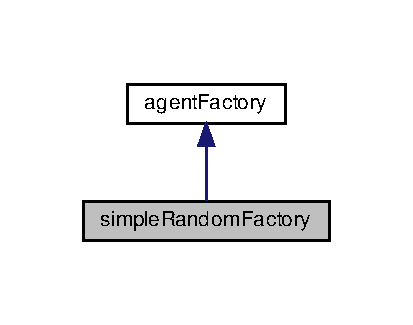
\includegraphics[width=198pt]{classsimpleRandomFactory__inherit__graph}
\end{center}
\end{figure}


Collaboration diagram for simple\+Random\+Factory\+:\nopagebreak
\begin{figure}[H]
\begin{center}
\leavevmode
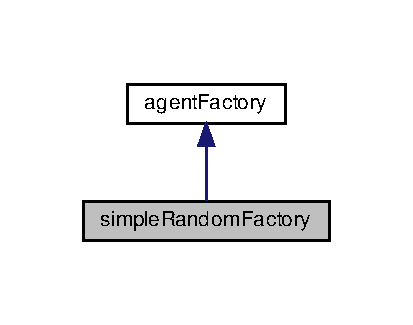
\includegraphics[width=198pt]{classsimpleRandomFactory__coll__graph}
\end{center}
\end{figure}
\subsection*{Private Member Functions}
\begin{DoxyCompactItemize}
\item 
\mbox{\Hypertarget{classsimpleRandomFactory_ac781683a570893f0fffef73f0d253aac}\label{classsimpleRandomFactory_ac781683a570893f0fffef73f0d253aac}} 
void {\bfseries create\+Agents} (vector$<$ \mbox{\hyperlink{classagent}{agent}} $\ast$$>$ \&\mbox{\hyperlink{classagents}{agents}})
\end{DoxyCompactItemize}
\subsection*{Additional Inherited Members}


\subsection{Detailed Description}


Definition at line 88 of file agent\+Factory.\+h.



The documentation for this class was generated from the following file\+:\begin{DoxyCompactItemize}
\item 
agent\+Factory.\+h\end{DoxyCompactItemize}

\hypertarget{classsimpleWorldpopFactory}{}\section{simple\+Worldpop\+Factory Class Reference}
\label{classsimpleWorldpopFactory}\index{simple\+Worldpop\+Factory@{simple\+Worldpop\+Factory}}


Inheritance diagram for simple\+Worldpop\+Factory\+:
\nopagebreak
\begin{figure}[H]
\begin{center}
\leavevmode
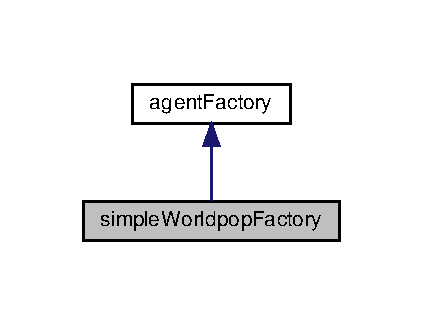
\includegraphics[width=203pt]{classsimpleWorldpopFactory__inherit__graph}
\end{center}
\end{figure}


Collaboration diagram for simple\+Worldpop\+Factory\+:
\nopagebreak
\begin{figure}[H]
\begin{center}
\leavevmode
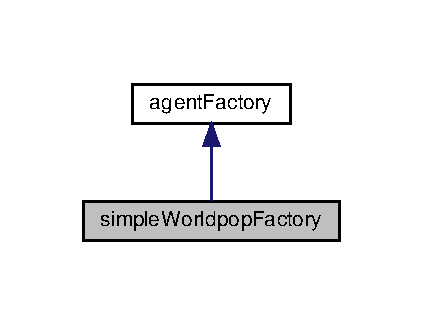
\includegraphics[width=203pt]{classsimpleWorldpopFactory__coll__graph}
\end{center}
\end{figure}
\subsection*{Private Member Functions}
\begin{DoxyCompactItemize}
\item 
\mbox{\Hypertarget{classsimpleWorldpopFactory_a5093cf767e45d5456f8cac1aba3a4649}\label{classsimpleWorldpopFactory_a5093cf767e45d5456f8cac1aba3a4649}} 
void {\bfseries create\+Agents} (vector$<$ \mbox{\hyperlink{classagent}{agent}} $\ast$$>$ \&\mbox{\hyperlink{classagents}{agents}})
\end{DoxyCompactItemize}
\subsection*{Additional Inherited Members}


\subsection{Detailed Description}


Definition at line 47 of file agent\+Factory.\+h.



The documentation for this class was generated from the following file\+:\begin{DoxyCompactItemize}
\item 
agent\+Factory.\+h\end{DoxyCompactItemize}

\hypertarget{structtimeTable}{}\section{time\+Table Struct Reference}
\label{structtimeTable}\index{time\+Table@{time\+Table}}


Collaboration diagram for time\+Table\+:\nopagebreak
\begin{figure}[H]
\begin{center}
\leavevmode
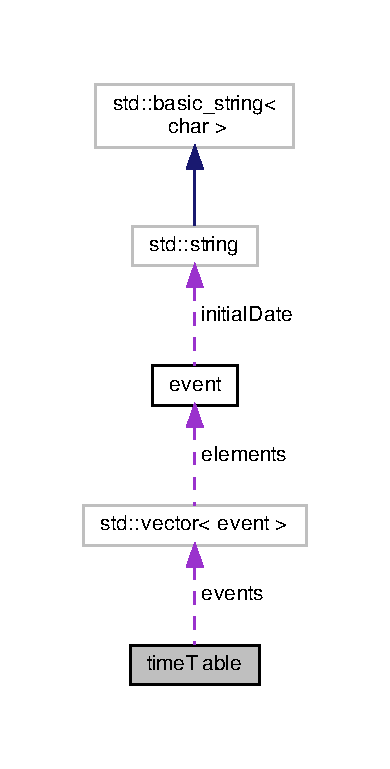
\includegraphics[width=187pt]{structtimeTable__coll__graph}
\end{center}
\end{figure}
\subsection*{Public Member Functions}
\begin{DoxyCompactItemize}
\item 
\mbox{\Hypertarget{structtimeTable_adfcfec62e9a80e6e4c1c3bea61f56b46}\label{structtimeTable_adfcfec62e9a80e6e4c1c3bea61f56b46}} 
void {\bfseries add} (string s, unsigned e)
\item 
\mbox{\Hypertarget{structtimeTable_a56ad08bdfbfa3e9ed26150ad340cbcbd}\label{structtimeTable_a56ad08bdfbfa3e9ed26150ad340cbcbd}} 
void {\bfseries change\+Event\+Time} (int i, int tick)
\item 
\mbox{\Hypertarget{structtimeTable_a10463383ade0b811376d5cfe3e3a52e1}\label{structtimeTable_a10463383ade0b811376d5cfe3e3a52e1}} 
void {\bfseries change\+Event\+Time} (int i, string s)
\item 
\mbox{\Hypertarget{structtimeTable_ac2424fec4a3b8ed8d3d53a47cc75794c}\label{structtimeTable_ac2424fec4a3b8ed8d3d53a47cc75794c}} 
void {\bfseries add\+Minutes\+To\+Event\+Time} (int i, int m)
\item 
\mbox{\Hypertarget{structtimeTable_ad440c828f6bd84b5de35a47d8b1fcc90}\label{structtimeTable_ad440c828f6bd84b5de35a47d8b1fcc90}} 
void {\bfseries add\+Seconds\+To\+Event\+Time} (int i, int s)
\item 
\mbox{\Hypertarget{structtimeTable_a051a72dbd35fc2fe344ec45d32c8d143}\label{structtimeTable_a051a72dbd35fc2fe344ec45d32c8d143}} 
\mbox{\hyperlink{structevent}{event}} \& {\bfseries get\+Current} ()
\item 
\mbox{\Hypertarget{structtimeTable_a952cb5000c669cfc61241f7abfade276}\label{structtimeTable_a952cb5000c669cfc61241f7abfade276}} 
\mbox{\hyperlink{structevent}{event}} \& {\bfseries get\+Previous} ()
\item 
\mbox{\Hypertarget{structtimeTable_a5d435684eb3fd7ca8be8bc4becfbb3a5}\label{structtimeTable_a5d435684eb3fd7ca8be8bc4becfbb3a5}} 
bool {\bfseries after} (ptime p, \mbox{\hyperlink{structevent}{event}} e)
\item 
\mbox{\Hypertarget{structtimeTable_aa82f1bfce0bf3d1cbc828a1c0776a35d}\label{structtimeTable_aa82f1bfce0bf3d1cbc828a1c0776a35d}} 
bool {\bfseries update} ()
\item 
\mbox{\Hypertarget{structtimeTable_af6ff36f262be339c23c027d90f202ec1}\label{structtimeTable_af6ff36f262be339c23c027d90f202ec1}} 
void {\bfseries bell} ()
\end{DoxyCompactItemize}
\subsection*{Public Attributes}
\begin{DoxyCompactItemize}
\item 
\mbox{\Hypertarget{structtimeTable_acf9d92d0c3b773312ee18e4df1c4ef24}\label{structtimeTable_acf9d92d0c3b773312ee18e4df1c4ef24}} 
vector$<$ \mbox{\hyperlink{structevent}{event}} $>$ {\bfseries events}
\item 
\mbox{\Hypertarget{structtimeTable_a23a883cdef1355fe2b074ac738f432cf}\label{structtimeTable_a23a883cdef1355fe2b074ac738f432cf}} 
int {\bfseries current}
\end{DoxyCompactItemize}


\subsection{Detailed Description}


Definition at line 30 of file timetable.\+h.



The documentation for this struct was generated from the following file\+:\begin{DoxyCompactItemize}
\item 
timetable.\+h\end{DoxyCompactItemize}

\hypertarget{classtiming}{}\section{timing Class Reference}
\label{classtiming}\index{timing@{timing}}


Collaboration diagram for timing\+:
\nopagebreak
\begin{figure}[H]
\begin{center}
\leavevmode
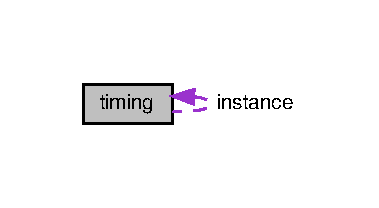
\includegraphics[width=182pt]{classtiming__coll__graph}
\end{center}
\end{figure}
\subsection*{Public Member Functions}
\begin{DoxyCompactItemize}
\item 
\mbox{\Hypertarget{classtiming_a5c91382984c1f17f3678030277bca2b7}\label{classtiming_a5c91382984c1f17f3678030277bca2b7}} 
void {\bfseries update} ()
\item 
\mbox{\Hypertarget{classtiming_aff54a0e908c64c52155ab254e4c16b31}\label{classtiming_aff54a0e908c64c52155ab254e4c16b31}} 
ptime {\bfseries now} () const
\item 
\mbox{\Hypertarget{classtiming_af7f37b61e8ad76615b81a9e620ed1b20}\label{classtiming_af7f37b61e8ad76615b81a9e620ed1b20}} 
date {\bfseries today} () const
\item 
\mbox{\Hypertarget{classtiming_a32e58b29ebab4444095da675a7366311}\label{classtiming_a32e58b29ebab4444095da675a7366311}} 
date {\bfseries tomorrow} () const
\item 
\mbox{\Hypertarget{classtiming_a386cc29fbab2bcb13c319fa5847e6c02}\label{classtiming_a386cc29fbab2bcb13c319fa5847e6c02}} 
date {\bfseries yesterday} () const
\item 
\mbox{\Hypertarget{classtiming_a89db990194b162a228a1db8497a78bdf}\label{classtiming_a89db990194b162a228a1db8497a78bdf}} 
date {\bfseries initial\+Day} () const
\item 
\mbox{\Hypertarget{classtiming_aa6fa7d6bb3338a83cf26deddab164dcd}\label{classtiming_aa6fa7d6bb3338a83cf26deddab164dcd}} 
ptime {\bfseries start\+Of\+School\+Day} () const
\item 
\mbox{\Hypertarget{classtiming_a44b6864a75b11c761eaaa6d6546f5c92}\label{classtiming_a44b6864a75b11c761eaaa6d6546f5c92}} 
ptime {\bfseries end\+Of\+School\+Day} () const
\item 
\mbox{\Hypertarget{classtiming_add6be686df899d4d114545f791ceb5d0}\label{classtiming_add6be686df899d4d114545f791ceb5d0}} 
date {\bfseries start\+Of\+School\+Term} () const
\item 
\mbox{\Hypertarget{classtiming_a672fd71230612e481b36eb408497c816}\label{classtiming_a672fd71230612e481b36eb408497c816}} 
date {\bfseries end\+Of\+School\+Term} () const
\item 
\mbox{\Hypertarget{classtiming_aa5bd281f145600c23293b94577799ca8}\label{classtiming_aa5bd281f145600c23293b94577799ca8}} 
date\+\_\+period {\bfseries half\+Term} () const
\item 
\mbox{\Hypertarget{classtiming_a79eb6645a9ccc90e59fc73594dc3b0c5}\label{classtiming_a79eb6645a9ccc90e59fc73594dc3b0c5}} 
date\+\_\+period {\bfseries term} () const
\item 
\mbox{\Hypertarget{classtiming_a251ccabb3906aaa811758eea285b32ac}\label{classtiming_a251ccabb3906aaa811758eea285b32ac}} 
time\+\_\+period {\bfseries school\+Day} () const
\item 
\mbox{\Hypertarget{classtiming_af80c4617bd5afd2f7c23a08f163bd465}\label{classtiming_af80c4617bd5afd2f7c23a08f163bd465}} 
time\+\_\+period {\bfseries lunch\+Time} () const
\item 
\mbox{\Hypertarget{classtiming_af39bf7bf9b0c1a4429ed3d228660fd8f}\label{classtiming_af39bf7bf9b0c1a4429ed3d228660fd8f}} 
time\+\_\+period {\bfseries morning\+Break\+Time} () const
\item 
\mbox{\Hypertarget{classtiming_a296ee7a0fce0144583b4ce632e669b89}\label{classtiming_a296ee7a0fce0144583b4ce632e669b89}} 
time\+\_\+period {\bfseries afternoon\+Break\+Time} () const
\end{DoxyCompactItemize}
\subsection*{Static Public Member Functions}
\begin{DoxyCompactItemize}
\item 
\mbox{\Hypertarget{classtiming_a9495f6f63b2c27f1af4ac4dc736fff10}\label{classtiming_a9495f6f63b2c27f1af4ac4dc736fff10}} 
static \mbox{\hyperlink{classtiming}{timing}} \& {\bfseries get\+Instance} ()
\end{DoxyCompactItemize}
\subsection*{Static Protected Attributes}
\begin{DoxyCompactItemize}
\item 
\mbox{\Hypertarget{classtiming_a599549bbe9902602897b50118793a2f7}\label{classtiming_a599549bbe9902602897b50118793a2f7}} 
static ptime {\bfseries current\+Time} =ptime(time\+\_\+from\+\_\+string(\char`\"{}2020-\/Mar-\/10 00\+:00\char`\"{}))
\item 
\mbox{\Hypertarget{classtiming_a0b97e2508018c7aced9978138c1a44ab}\label{classtiming_a0b97e2508018c7aced9978138c1a44ab}} 
static ptime {\bfseries start\+Time} =ptime(time\+\_\+from\+\_\+string(\char`\"{}2020-\/Mar-\/10 00\+:00\char`\"{}))
\item 
\mbox{\Hypertarget{classtiming_aa31635ef349e78a1689461213d316ed4}\label{classtiming_aa31635ef349e78a1689461213d316ed4}} 
static date {\bfseries start\+Date} =ptime(time\+\_\+from\+\_\+string(\char`\"{}2020-\/Mar-\/10 00\+:00\char`\"{})).date()
\item 
\mbox{\Hypertarget{classtiming_abbabc1091ef472ea1210d319889f1793}\label{classtiming_abbabc1091ef472ea1210d319889f1793}} 
static double {\bfseries time\+Step} =0
\end{DoxyCompactItemize}
\subsection*{Private Member Functions}
\begin{DoxyCompactItemize}
\item 
\mbox{\Hypertarget{classtiming_ae7c2f1ad143d9dc5f56d30ab447bcdd6}\label{classtiming_ae7c2f1ad143d9dc5f56d30ab447bcdd6}} 
{\bfseries timing} (const \mbox{\hyperlink{classtiming}{timing}} \&)=delete
\item 
\mbox{\Hypertarget{classtiming_a30b82d8d0d6ca5350e23cd34a9e1ba7e}\label{classtiming_a30b82d8d0d6ca5350e23cd34a9e1ba7e}} 
\mbox{\hyperlink{classtiming}{timing}} \& {\bfseries operator=} (const \mbox{\hyperlink{classtiming}{timing}} \&)=delete
\end{DoxyCompactItemize}
\subsection*{Static Private Member Functions}
\begin{DoxyCompactItemize}
\item 
\mbox{\Hypertarget{classtiming_a692446f24b88e08f46243324a5f85ff7}\label{classtiming_a692446f24b88e08f46243324a5f85ff7}} 
static void {\bfseries init\+Singleton} ()
\end{DoxyCompactItemize}
\subsection*{Static Private Attributes}
\begin{DoxyCompactItemize}
\item 
\mbox{\Hypertarget{classtiming_aa3ac445dda7e069d4df60be71fdabafe}\label{classtiming_aa3ac445dda7e069d4df60be71fdabafe}} 
static \mbox{\hyperlink{classtiming}{timing}} $\ast$ {\bfseries instance} = nullptr
\item 
\mbox{\Hypertarget{classtiming_a227481b54d97006b91aa6bd1cb2eec65}\label{classtiming_a227481b54d97006b91aa6bd1cb2eec65}} 
static std\+::once\+\_\+flag {\bfseries init\+Instance\+Flag}
\end{DoxyCompactItemize}


\subsection{Detailed Description}


Definition at line 21 of file timing.\+h.



The documentation for this class was generated from the following files\+:\begin{DoxyCompactItemize}
\item 
\mbox{\hyperlink{timing_8h}{timing.\+h}}\item 
timing.\+cpp\end{DoxyCompactItemize}

\chapter{File Documentation}
\hypertarget{agent_8h}{}\section{agent.\+h File Reference}
\label{agent_8h}\index{agent.\+h@{agent.\+h}}


The agent class definition file.  


{\ttfamily \#include \char`\"{}timetable.\+h\char`\"{}}\newline
{\ttfamily \#include \char`\"{}paths.\+h\char`\"{}}\newline
{\ttfamily \#include \char`\"{}process.\+h\char`\"{}}\newline
{\ttfamily \#include \char`\"{}places.\+h\char`\"{}}\newline
{\ttfamily \#include \char`\"{}model.\+h\char`\"{}}\newline
{\ttfamily \#include \char`\"{}disease.\+h\char`\"{}}\newline
Include dependency graph for agent.\+h\+:
\nopagebreak
\begin{figure}[H]
\begin{center}
\leavevmode
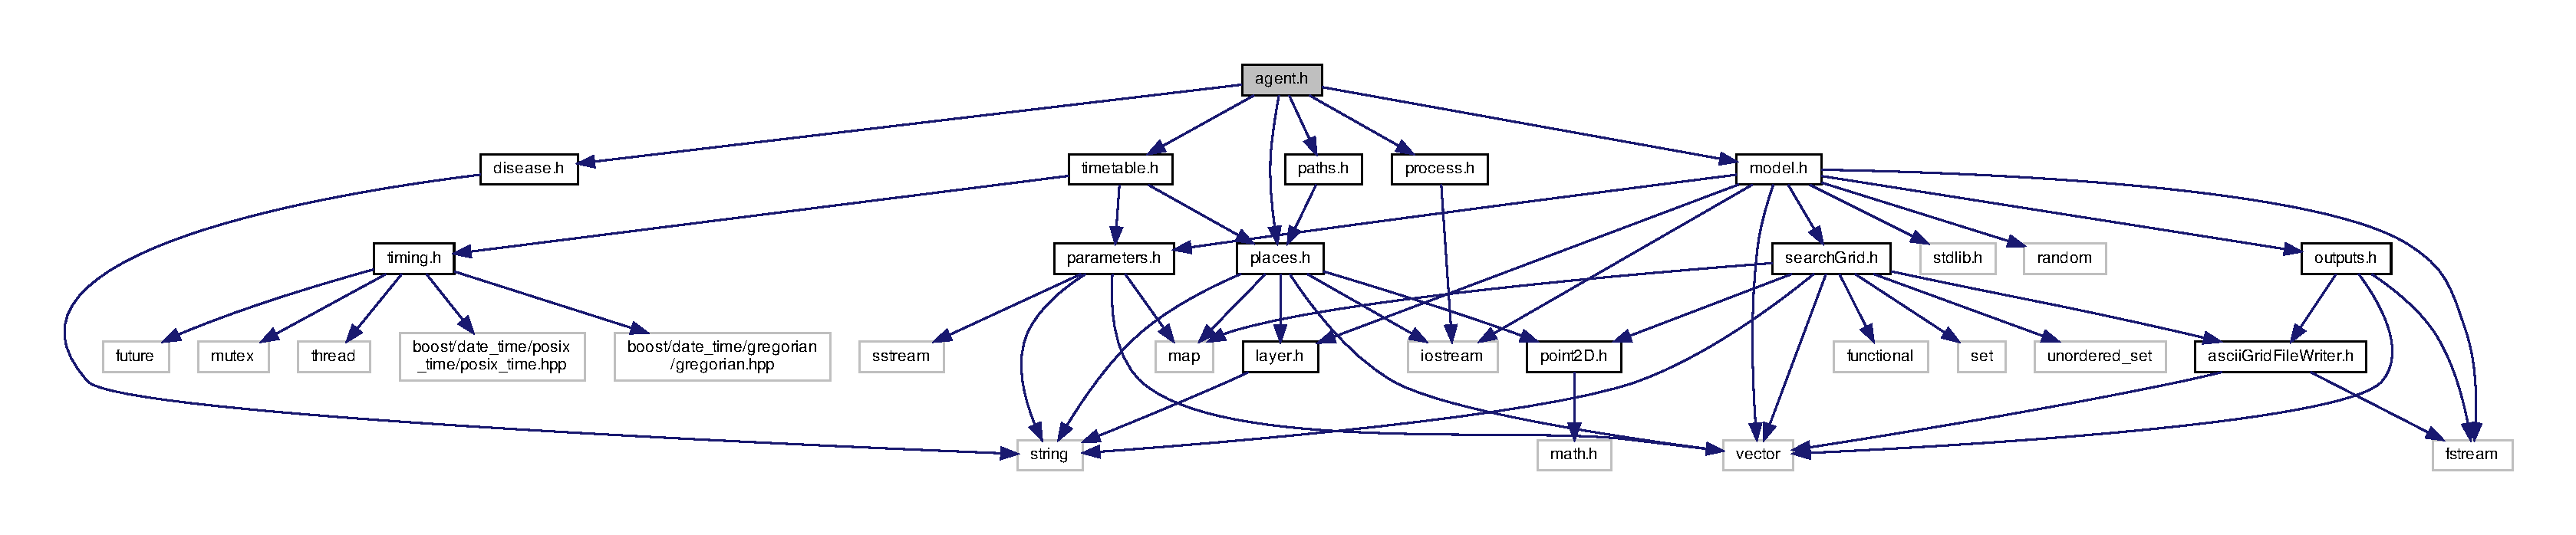
\includegraphics[width=350pt]{agent_8h__incl}
\end{center}
\end{figure}
This graph shows which files directly or indirectly include this file\+:
\nopagebreak
\begin{figure}[H]
\begin{center}
\leavevmode
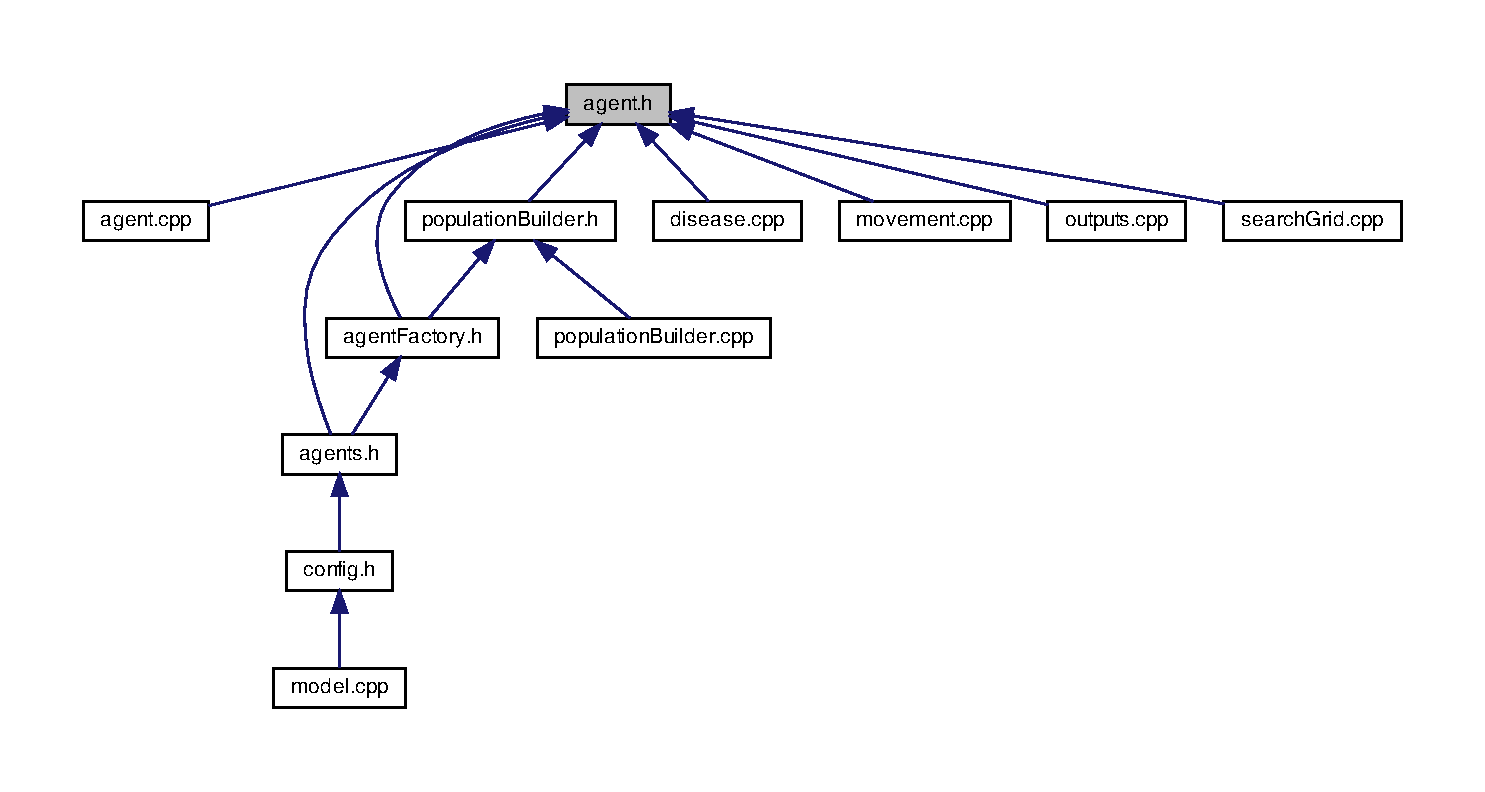
\includegraphics[width=350pt]{agent_8h__dep__incl}
\end{center}
\end{figure}
\subsection*{Classes}
\begin{DoxyCompactItemize}
\item 
class \mbox{\hyperlink{classagent}{agent}}
\end{DoxyCompactItemize}


\subsection{Detailed Description}
The agent class definition file. 

\begin{DoxyAuthor}{Author}
Mike Bithell 
\end{DoxyAuthor}

\hypertarget{model_8cpp}{}\section{model.\+cpp File Reference}
\label{model_8cpp}\index{model.\+cpp@{model.\+cpp}}


This is the model implementation.  


{\ttfamily \#include \char`\"{}model.\+h\char`\"{}}\newline
{\ttfamily \#include \char`\"{}parameters.\+h\char`\"{}}\newline
{\ttfamily \#include \char`\"{}timing.\+h\char`\"{}}\newline
{\ttfamily \#include \char`\"{}config.\+h\char`\"{}}\newline
{\ttfamily \#include \char`\"{}movement.\+h\char`\"{}}\newline
{\ttfamily \#include $<$boost/filesystem.\+hpp$>$}\newline
{\ttfamily \#include $<$functional$>$}\newline
Include dependency graph for model.\+cpp\+:\nopagebreak
\begin{figure}[H]
\begin{center}
\leavevmode
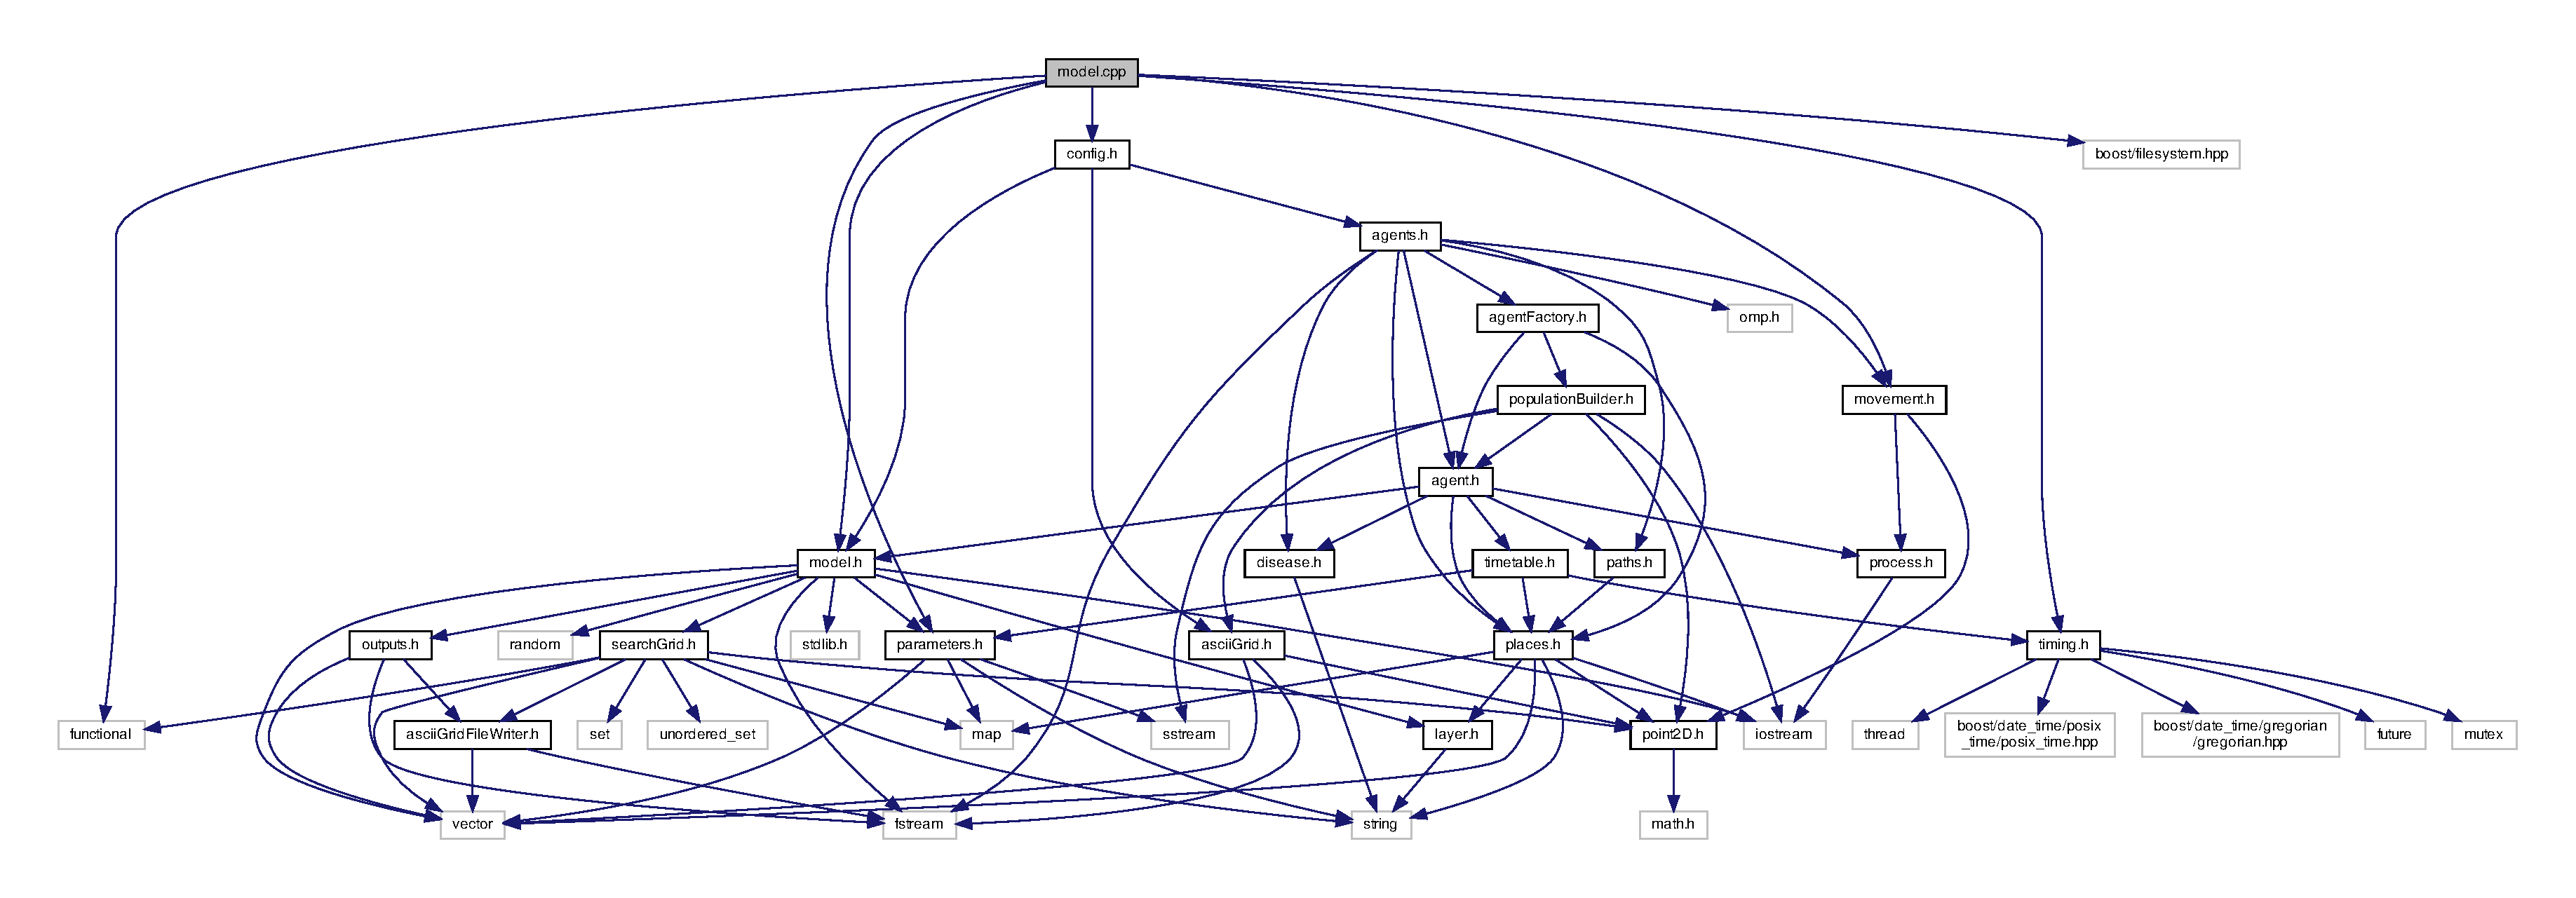
\includegraphics[width=350pt]{model_8cpp__incl}
\end{center}
\end{figure}


\subsection{Detailed Description}
This is the model implementation. 


\hypertarget{model_8h}{}\section{model.\+h File Reference}
\label{model_8h}\index{model.\+h@{model.\+h}}


This is the model class header file.  


{\ttfamily \#include $<$vector$>$}\newline
{\ttfamily \#include $<$iostream$>$}\newline
{\ttfamily \#include $<$fstream$>$}\newline
{\ttfamily \#include \char`\"{}stdlib.\+h\char`\"{}}\newline
{\ttfamily \#include \char`\"{}layer.\+h\char`\"{}}\newline
{\ttfamily \#include \char`\"{}search\+Grid.\+h\char`\"{}}\newline
{\ttfamily \#include \char`\"{}parameters.\+h\char`\"{}}\newline
{\ttfamily \#include \char`\"{}outputs.\+h\char`\"{}}\newline
{\ttfamily \#include $<$random$>$}\newline
Include dependency graph for model.\+h\+:\nopagebreak
\begin{figure}[H]
\begin{center}
\leavevmode
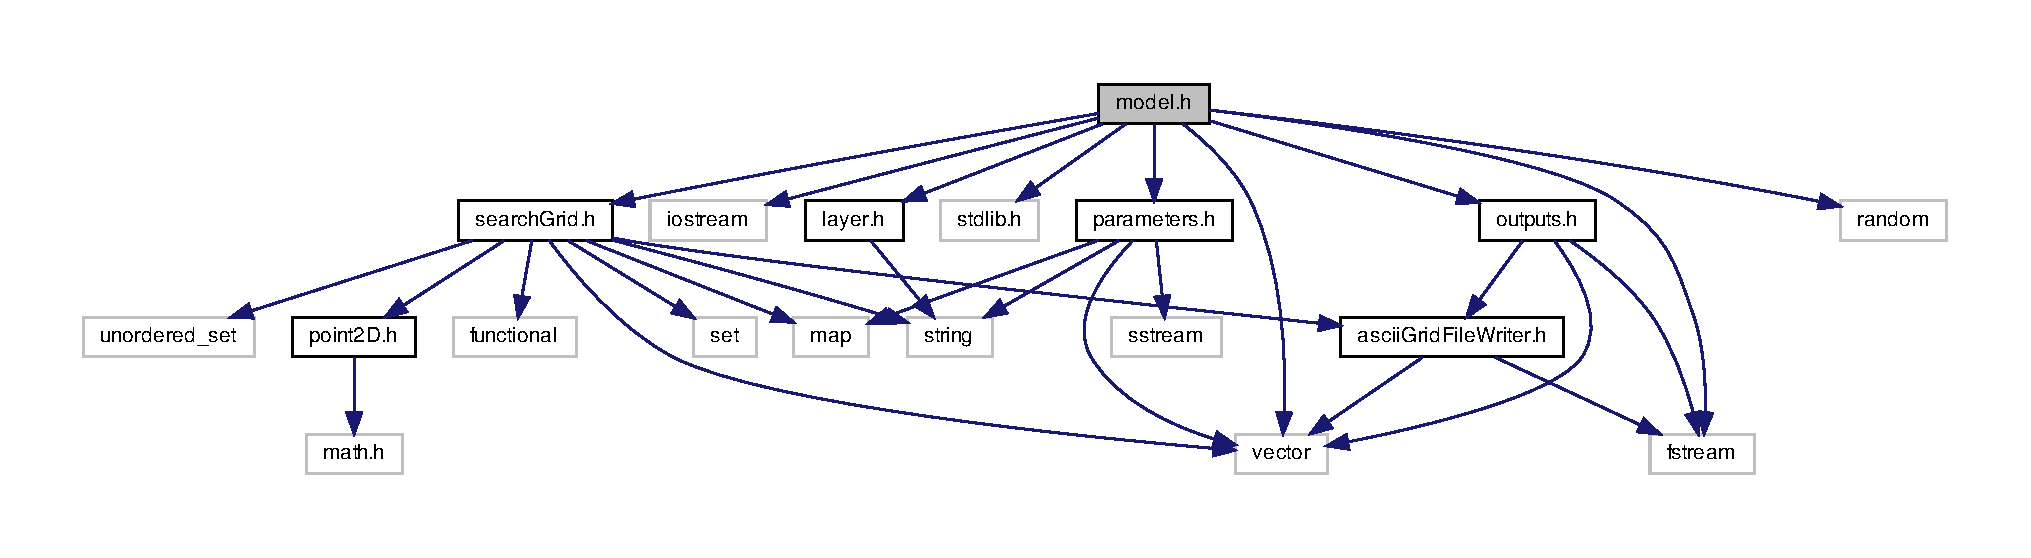
\includegraphics[width=350pt]{model_8h__incl}
\end{center}
\end{figure}
This graph shows which files directly or indirectly include this file\+:\nopagebreak
\begin{figure}[H]
\begin{center}
\leavevmode
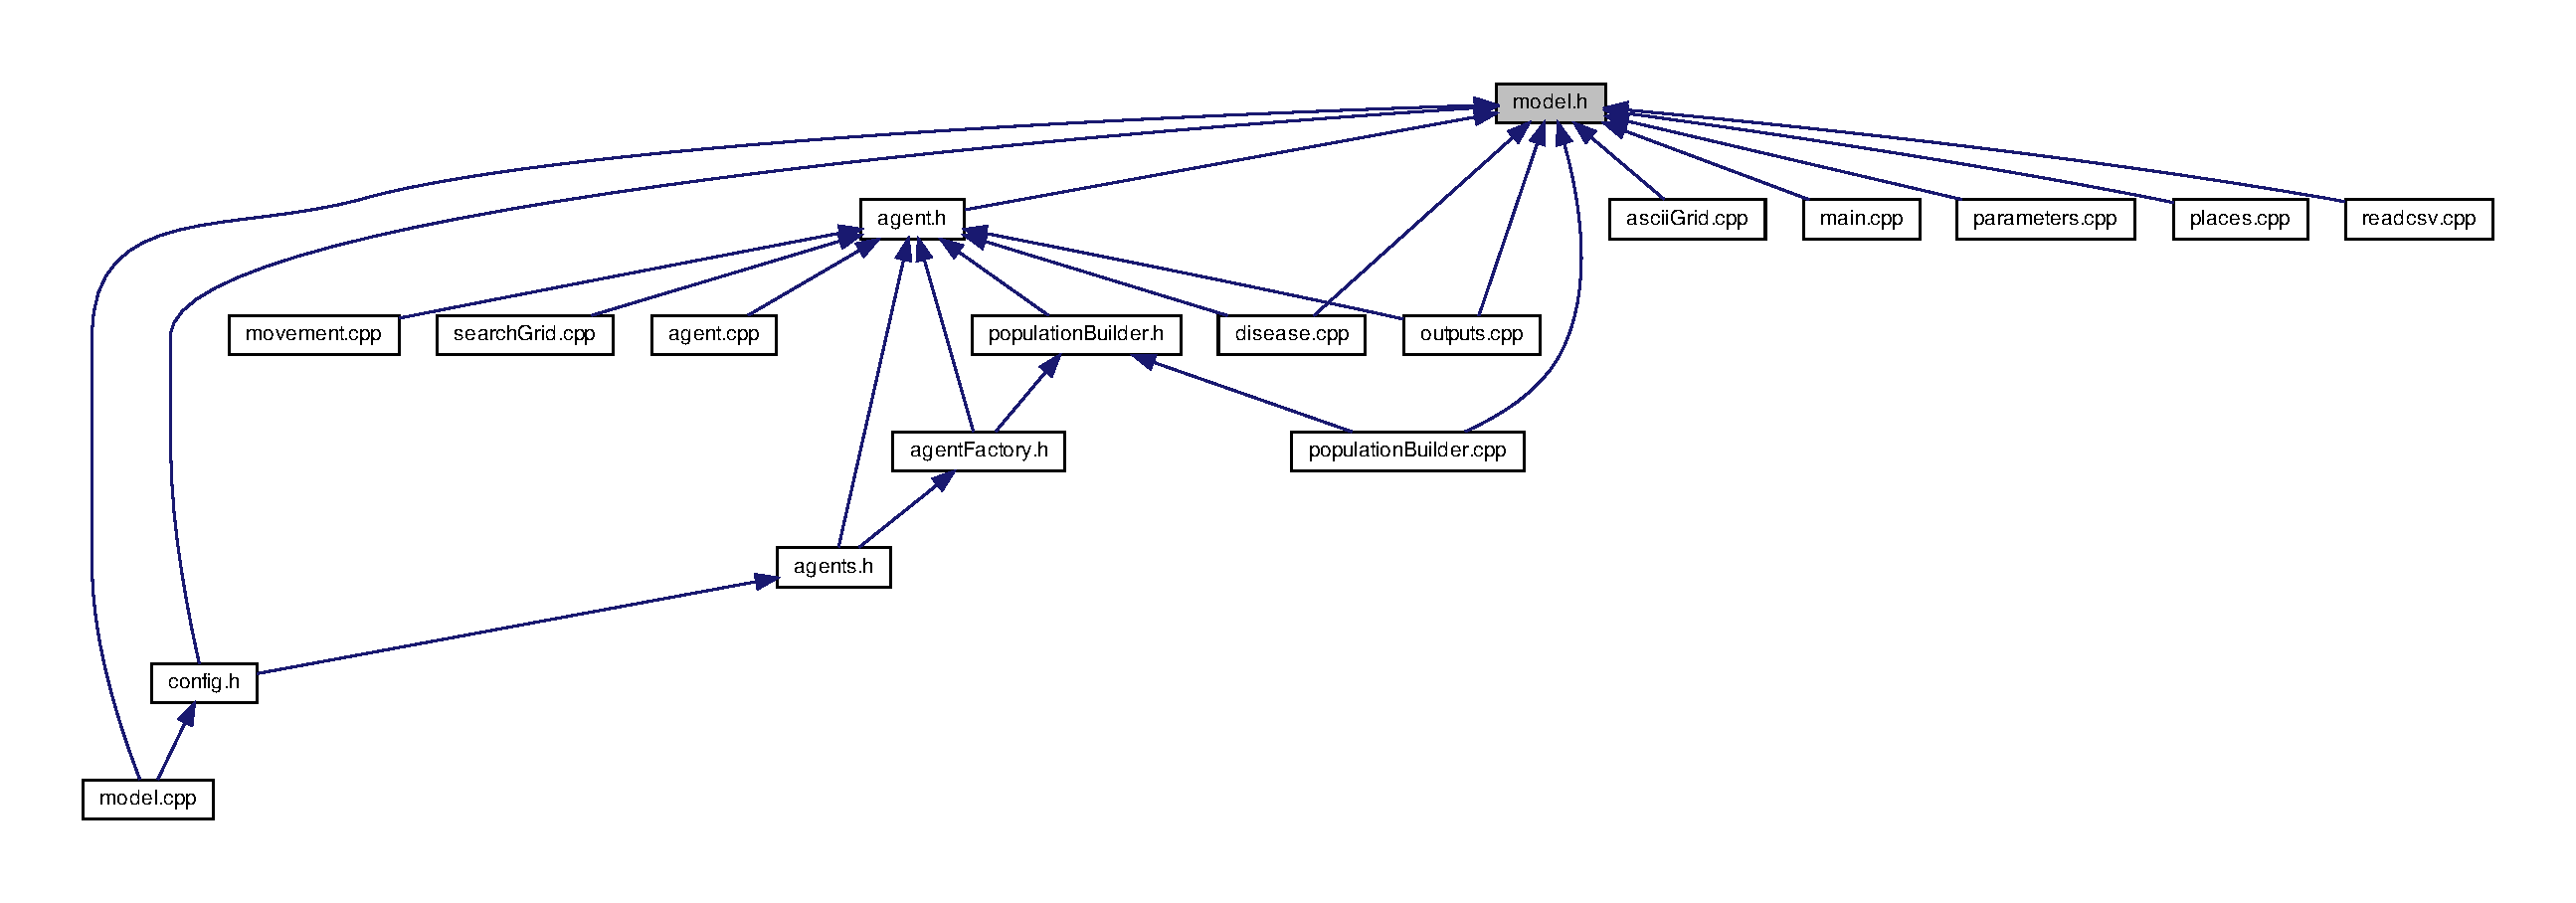
\includegraphics[width=350pt]{model_8h__dep__incl}
\end{center}
\end{figure}
\subsection*{Classes}
\begin{DoxyCompactItemize}
\item 
class \mbox{\hyperlink{classrandomizer}{randomizer}}
\item 
class \mbox{\hyperlink{classmodel}{model}}
\begin{DoxyCompactList}\small\item\em The model holds the agents in a vector and drives their updates. \end{DoxyCompactList}\end{DoxyCompactItemize}


\subsection{Detailed Description}
This is the model class header file. 


\hypertarget{parameters_8h}{}\section{parameters.\+h File Reference}
\label{parameters_8h}\index{parameters.\+h@{parameters.\+h}}


The parameters class header file.  


{\ttfamily \#include $<$string$>$}\newline
{\ttfamily \#include $<$sstream$>$}\newline
{\ttfamily \#include $<$vector$>$}\newline
{\ttfamily \#include $<$map$>$}\newline
Include dependency graph for parameters.\+h\+:\nopagebreak
\begin{figure}[H]
\begin{center}
\leavevmode
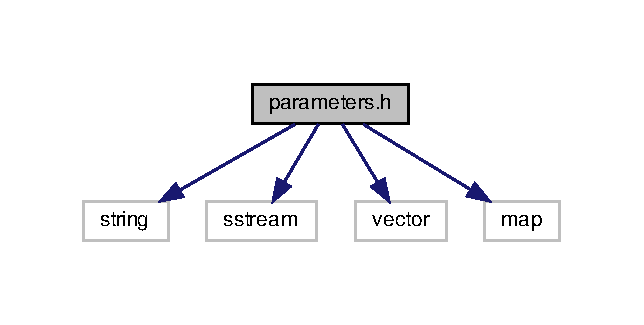
\includegraphics[width=309pt]{parameters_8h__incl}
\end{center}
\end{figure}
This graph shows which files directly or indirectly include this file\+:\nopagebreak
\begin{figure}[H]
\begin{center}
\leavevmode
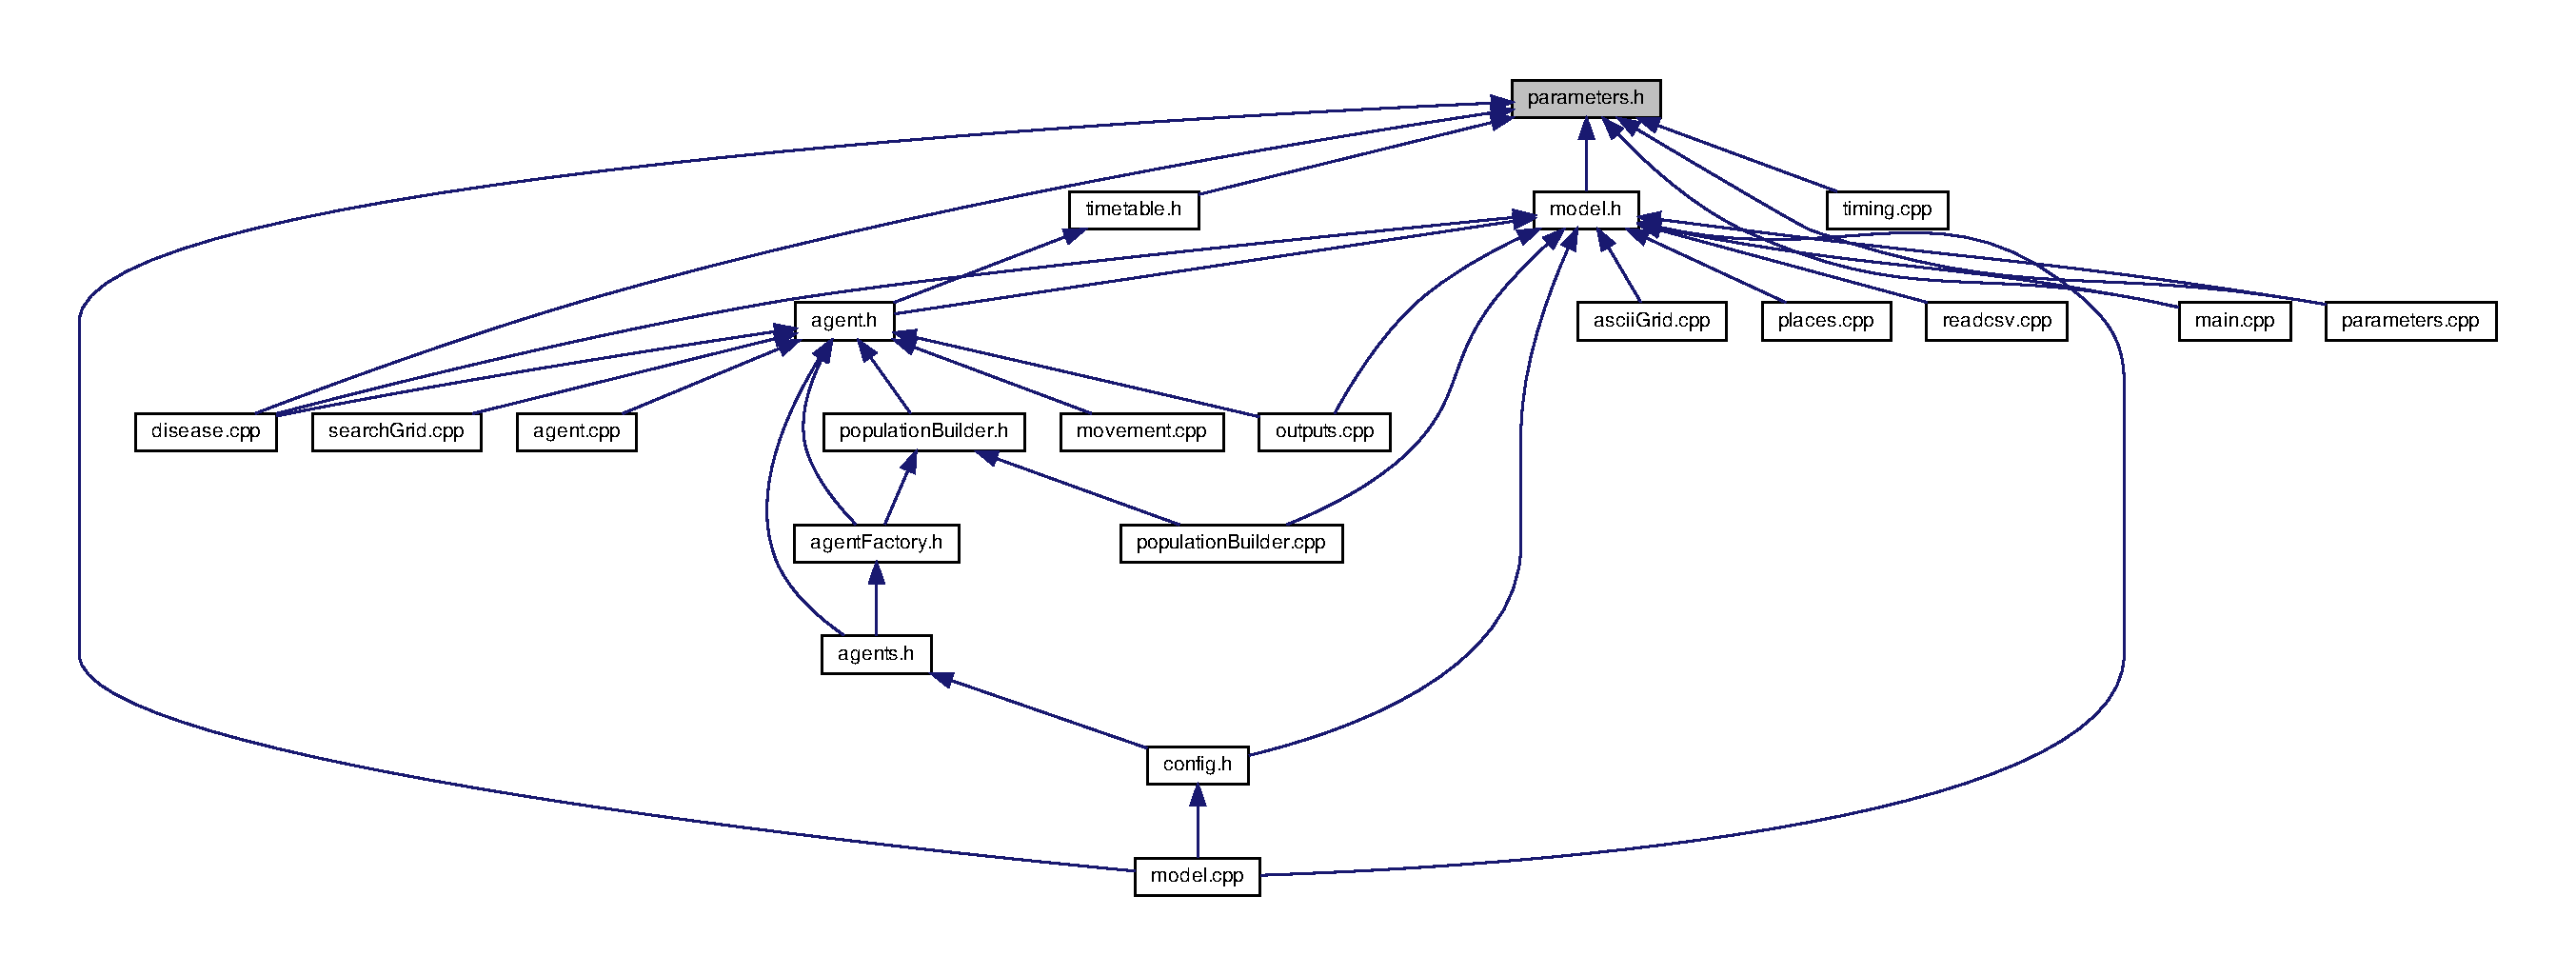
\includegraphics[width=350pt]{parameters_8h__dep__incl}
\end{center}
\end{figure}
\subsection*{Classes}
\begin{DoxyCompactItemize}
\item 
class \mbox{\hyperlink{classparameters}{parameters}}
\end{DoxyCompactItemize}


\subsection{Detailed Description}
The parameters class header file. 

This class stores a set of model parameters. It is a singleton. 
\hypertarget{timing_8h}{}\section{timing.\+h File Reference}
\label{timing_8h}\index{timing.\+h@{timing.\+h}}


The time class header file.  


{\ttfamily \#include \char`\"{}boost/date\+\_\+time/posix\+\_\+time/posix\+\_\+time.\+hpp\char`\"{}}\newline
{\ttfamily \#include \char`\"{}boost/date\+\_\+time/gregorian/gregorian.\+hpp\char`\"{}}\newline
{\ttfamily \#include $<$future$>$}\newline
{\ttfamily \#include $<$mutex$>$}\newline
{\ttfamily \#include $<$thread$>$}\newline
Include dependency graph for timing.\+h\+:\nopagebreak
\begin{figure}[H]
\begin{center}
\leavevmode
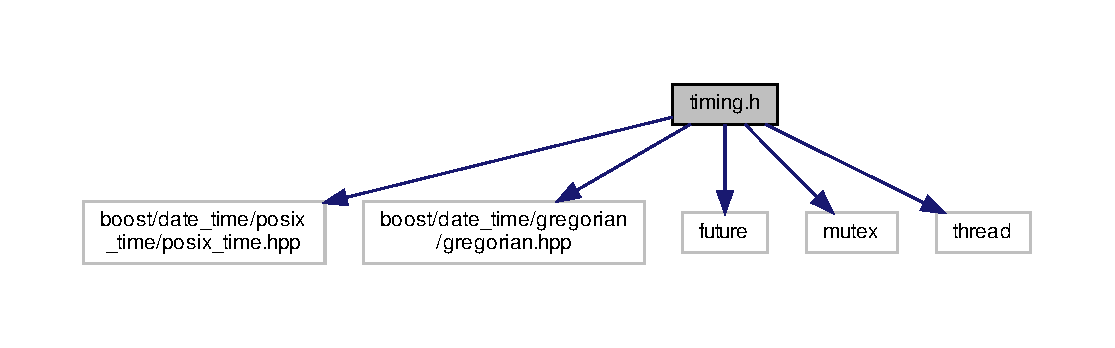
\includegraphics[width=350pt]{timing_8h__incl}
\end{center}
\end{figure}
This graph shows which files directly or indirectly include this file\+:\nopagebreak
\begin{figure}[H]
\begin{center}
\leavevmode
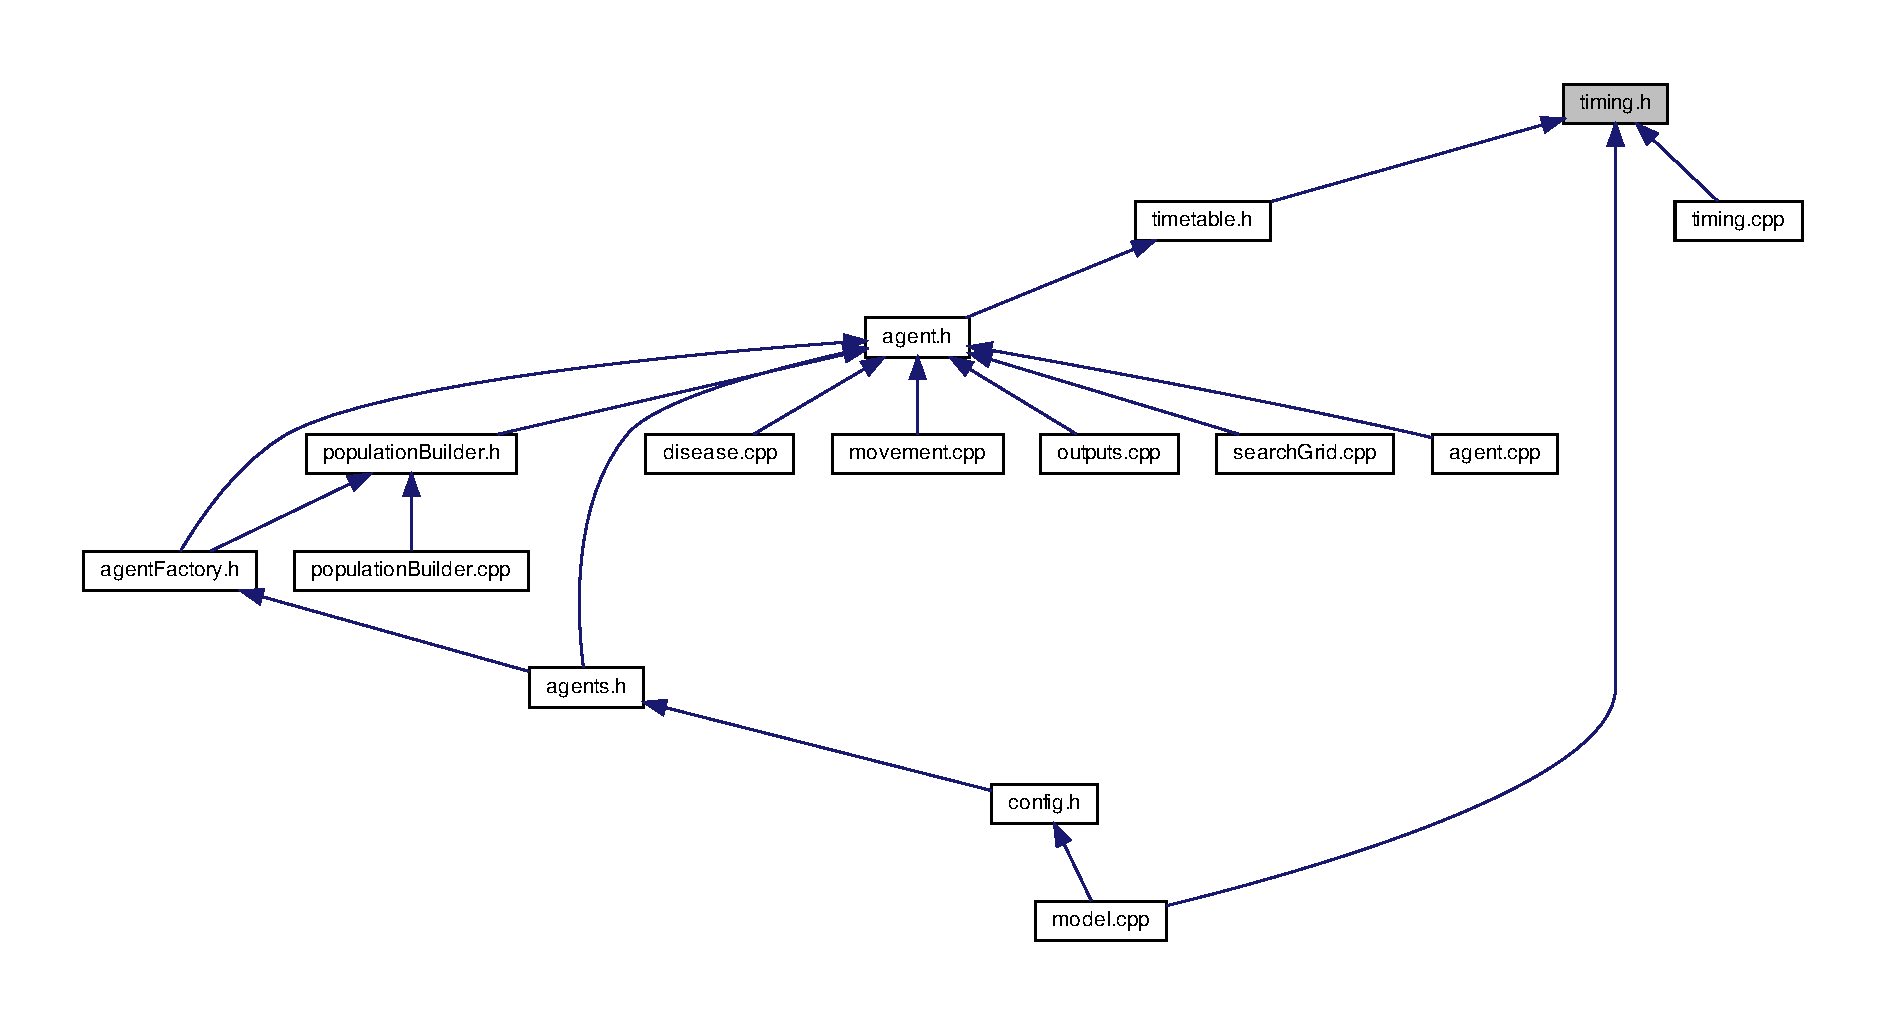
\includegraphics[width=350pt]{timing_8h__dep__incl}
\end{center}
\end{figure}
\subsection*{Classes}
\begin{DoxyCompactItemize}
\item 
class \mbox{\hyperlink{classtiming}{timing}}
\end{DoxyCompactItemize}


\subsection{Detailed Description}
The time class header file. 

This class abstracts the handling of time so that timesteps can be mapped to real time values such as hours and days. This is a singleton so the constructor cannot be called directly. The class uses the boost Date Time library to make calculation of times easy. The initial time\+Step provided by the input file is expected to be in seconds. 
%--- End generated contents ---

% Index
\backmatter
\newpage
\phantomsection
\clearemptydoublepage
\addcontentsline{toc}{chapter}{Index}
\printindex

\end{document}
